% 12pt: grandezza carattere
% a4paper: formato a4
% openright: apre i capitoli a destra
% twoside: serve per fare un
% documento fronteretro (oneside altrimenti)
% report: stile tesi (oppure book)
\documentclass[12pt,a4paper,openright,oneside]{report}

% libreria per scrivere in italiano
\usepackage[italian]{babel}

% libreria per accettare i caratteri
\usepackage[T1]{fontenc}
\usepackage[utf8]{inputenc}
\usepackage{adjustbox}
\usepackage{soul}

% libreria per impostare il documento
\usepackage{fancyhdr}
\usepackage{diagbox}


% libreria per avere l'indentazione all'inizio dei capitoli
\usepackage{indentfirst}

% libreria per inserire grafici
\usepackage{graphicx}

% libreria per utilizzare font particolari ad esempio \textsc{}
\usepackage{newlfont}

% libreria per inserire testo barrato (striked-out)
\usepackage[normalem]{ulem}

% Permette di avere la sottolineatura attaccata alla parola. Commentare per default
\setuldepth{come}

% Permette di avere citazioni con un background diverso
\usepackage[most]{tcolorbox}
\usepackage{lipsum}

\definecolor{backquote}{RGB}{242, 242, 242}

\newtcolorbox{myquote}[1][]{%
	enhanced, breakable, 
	size=normal,
	frame hidden, boxrule=10pt,
	sharp corners,
	colback=backquote,
	#1
}

% libreria per elenchi numerati nested (es. 1.1)
\usepackage{enumitem}

% libreria per tabelle multipagina
\usepackage{longtable}

% libreria per il rowspan e il colspan
\usepackage{multirow, multicol}
\newcommand{\sr}{\rule[-0.45cm]{0pt}{1.4cm}}

%
%%%%%%%%%%%%%%%%%%%%%%%%%%%%%%%%%%%%%%%%%libreria per tabelle multipagina
\usepackage{xcolor}

%
%%%%%%%%%%%%%%%%%%%%%%%%%%%%%%%%%%%%%%%%%libreria per tabelle multipagina
										%	con colonne centrate
\usepackage{array}
%
%%%%%%%%%%%%%%%%%%%%%%%%%%%%%%%%%%%%%%%%%libreria per produrre pagine landscape
										%	in un documento principalmente portrait
\usepackage{pdflscape}
%
%%%%%%%%%%%%%%%%%%%%%%%%%%%%%%%%%%%%%%%%%libreria per l'inserimento di link nella
                                        %   bibliografia
\PassOptionsToPackage{hyphens}{url}\usepackage[hidelinks]{hyperref}

% Per poter splittare bibliografica e sitografia
%\usepackage[backend=biber, style=numeric, defernumbers]{biblatex}
\usepackage[backend=bibtex,
style=numeric,
%style=alphabetic,
bibencoding=ascii,
%style=reading,
sorting=ynt
]{biblatex}
\addbibresource{relazione}

%
%%%%%%%%%%%%%%%%%%%%%%%%%%%%%%%%%%%%%%%%%libreria per l'inserimento testuale
										%	di frecce direzionali
\usepackage{textcomp}
%
%%%%%%%%%%%%%%%%%%%%%%%%%%%%%%%%%%%%%%%%%comando per l'inserimento di tab
\newcommand\tab[1][0,2cm]{\hspace*{#1}}
\newcommand\longtab[1][0,5cm]{\hspace*{#1}}
%
%%%%%%%%%%%%%%%%%%%%%%%%%%%%%%%%%%%%%%%%%comando per la gestione semplificata di quotes
\newcommand{\quotes}[1]{``#1''}
%%%%%%%%%%%%%%%%%%%%%%%%%%%%%%%%%%%%%%%%%comando per la gestione di legende a formule
\newenvironment{conditions}
{\par\vspace{\abovedisplayskip}\noindent\begin{tabular}{>{$}l<{$} @{${}={}$} l}}
	{\end{tabular}\par\vspace{\belowdisplayskip}}
%%%%%%%%%%%%%%%%%%%%%%%%%%%%%%%%%%%%%%%%%comando per il custom font size
\makeatletter
\newcommand{\codesize}{\@setfontsize{\srcsize}{7pt}{7pt}}
\makeatother
%
%%%%%%%%%%%%%%%%%%%%%%%%%%%%%%%%%%%%%%%%%librerie matematiche
\usepackage{amssymb}
\usepackage{amsmath}
\usepackage{latexsym}
\usepackage{amsthm}
%
%%%%%%%%%%%%%%%%%%%%%%%%%%%%%%%%%%%%%%%%%libreria per la visualizzazione di tree
\usepackage{dirtree}
%
%%%%%%%%%%%%%%%%%%%%%%%%%%%%%%%%%%%%%%%%%librerie per la visualizzazione del codice
\usepackage{listings}
\usepackage{color}
\definecolor{dkgreen}{rgb}{0,0.6,0}
\definecolor{gray}{rgb}{0.5,0.5,0.5}
\definecolor{redstrings}{rgb}{0.58,0,0.82}
\lstset{
	language=Java,
	captionpos=b,
	numbers=left,
	numberstyle=\tiny\color{gray},
	frame=tblr,
	tabsize=4, % tab space width
	showspaces=false,
	showtabs=false,
	breaklines=true,
	showstringspaces=false,
	breakatwhitespace=true,
	escapeinside={(*@}{@*)},
	basicstyle=\ttfamily\codesize,
	keywordstyle=\color{blue},
	commentstyle=\color{dkgreen},
	stringstyle=\color{redstrings}
}


\definecolor{delim}{RGB}{20,105,176}
\definecolor{numb}{RGB}{106, 109, 32}
\definecolor{string}{rgb}{0.64,0.08,0.08}
\definecolor{stringDark}{rgb}{0.34,0.34,0.64}


\lstdefinelanguage{json}{
	numbers=left,
	numberstyle=\tiny\color{gray},
	frame=single,
	rulecolor=\color{black},
	showspaces=false,
	showtabs=false,
	breaklines=true,
	postbreak=\raisebox{0ex}[0ex][0ex]{\ensuremath{\color{gray}\hookrightarrow\space}},
	breakatwhitespace=true,
	basicstyle=\ttfamily\codesize,
	upquote=true,
	morestring=[b]",
	stringstyle=\color{string},
	tabsize=2,
	identifierstyle=\namespaces,
	literate=
	*{0}{{{\color{numb}0}}}{1}
	{1}{{{\color{numb}1}}}{1}
	{2}{{{\color{numb}2}}}{1}
	{3}{{{\color{numb}3}}}{1}
	{4}{{{\color{numb}4}}}{1}
	{5}{{{\color{numb}5}}}{1}
	{6}{{{\color{numb}6}}}{1}
	{7}{{{\color{numb}7}}}{1}
	{8}{{{\color{numb}8}}}{1}
	{9}{{{\color{numb}9}}}{1}
	{\{}{{{\color{delim}{\{}}}}{1}
	{\}}{{{\color{delim}{\}}}}}{1}
	{[}{{{\color{delim}{[}}}}{1}
	{]}{{{\color{delim}{]}}}}{1}
	{"actions"}{{{\color{stringDark}{actions}}}}{9}
	{"properties"}{{{\color{stringDark}{properties}}}}{12}
	{"@context"}{{{\color{stringDark}{"@context"}}}}{10}
	{"@id"}{{{\color{stringDark}{"id"}}}}{5}
	{"@type"}{{{\color{stringDark}{"@type"}}}}{7},
}

\definecolor{lightgray}{rgb}{.9,.9,.9}
\definecolor{darkgray}{rgb}{.4,.4,.4}
\definecolor{purple}{rgb}{0.65, 0.12, 0.82}

\lstdefinelanguage{JavaScript}{
	keywords={typeof, new, true, false, catch, function, return, null, catch, switch, var, if, in, while, do, else, case, break, async, await, let, const},
	keywordstyle=\color{blue}\bfseries,
	ndkeywords={class, export, boolean, throw, implements, import, this, require},
	ndkeywordstyle=\color{darkgray}\bfseries,
	identifierstyle=\color{black},
	sensitive=false,
	basicstyle=\ttfamily\codesize,
	comment=[l]{//},
	morecomment=[s]{/*}{*/},
	commentstyle=\color{purple}\ttfamily,
	stringstyle=\color{red}\ttfamily,
	morestring=[b]',
	morestring=[b]"
}

\definecolor{gray}{rgb}{0.4,0.4,0.4}
\definecolor{darkblue}{rgb}{0.0,0.0,0.6}
\definecolor{cyan}{rgb}{0.0,0.6,0.6}

\lstdefinelanguage{XML}
{
	morestring=[b]",
	morestring=[s]{>}{<},
	morecomment=[s]{<?}{?>},
	stringstyle=\color{black},
	identifierstyle=\color{darkblue},
	keywordstyle=\color{cyan},
	morekeywords={xmlns,version,type}% list your attributes here
}

%
%%%%%%%%%%%%%%%%%%%%%%%%%%%%%%%%%%%%%%%%%3d graph
\usepackage{pgfplots}
\usepackage{pgfplotstable}
\pgfplotsset{width=12cm,compat=1.8}
%
%%%%%%%%%%%%%%%%%%%%%%%%%%%%%%%%%%%%%%%%%multiline comments
\usepackage{verbatim}


\usepackage[font={small,it}]{caption}


%
%%%%%%%%%%%%%%%%%%%%%%%%%%%%%%%%%%%%%%%%%impostazioni per il cambiamento di titolo
										%	in lstlistoflistings
\renewcommand\lstlistingname{Codice}
\renewcommand\lstlistlistingname{Elenco dei codici}
\def\lstlistingautorefname{Codice}
%
\oddsidemargin=30pt \evensidemargin=20pt	%impostano i margini

% Imposta la sillabazione per le parole che latex spezza male (senza virgole)
\hyphenation{sil-la-ba-zio-ne thread findbugs package gradle dev In-ter-ac-tion-Af-for-dance POST}


%%%%%%%%%%%%%%%%%%%%%%%%%%%%%%%%%%%%%%%%%comandi per l'impostazione
                                        %   della pagina, vedi il manuale
                                        %   della libreria fancyhdr
                                        %   per ulteriori delucidazioni
\pagestyle{fancy}\addtolength{\headwidth}{20pt}
\renewcommand{\chaptermark}[1]{\markboth{\thechapter.\ #1}{}}
\renewcommand{\sectionmark}[1]{\markright{\thesection \ #1}{}}
\rhead[\fancyplain{}{\bfseries\leftmark}]{\fancyplain{}{\bfseries\thepage}}
\cfoot{}
%%%%%%%%%%%%%%%%%%%%%%%%%%%%%%%%%%%%%%%%%
\linespread{1.3}                        %comando per impostare l'interlinea
%%%%%%%%%%%%%%%%%%%%%%%%%%%%%%%%%%%%%%%%%definisce nuovi comandi
%

\begin{document}
\begin{titlepage}
	\begin{center}
		\topskip0pt
		
		\vspace*{40mm}
		{\Large{\textbf{Semantic Smart Room}}}\\
		
		\vspace*{4mm}
		{\small{\textit{\url{https://github.com/Martinocom/pervasive-semantic-exam}}}}\\
		
		\vspace*{4mm}
		{\Large{Progettazione, creazione e l'uso delle Web Things all'interno di una stanza, utilizzando Agenti e metodologie di descrizione semantica}}\\
		
		\vspace{10mm}
		{\Large{Marcin Pabich\\}}
		{\large{0000835166}}
		
		\vspace{10mm}
		{\large{Gennaio 2021}}\\
		
		\vspace{20mm}
		{\large{\bf Università di Bologna}}\\
		\vspace{1mm}
		{\large{\bf Ingegneria e Scienze informatiche}}\\
		\vspace{1mm}
		{\large{\bf Anno Accademico 2019/2020}}
		\vspace*{\fill}
	\end{center}
\end{titlepage}
\pagenumbering{roman}                   %serve per mettere i numeri romani
\tableofcontents                        %crea l'indice
%%%%%%%%%%%%%%%%%%%%%%%%%%%%%%%%%%%%%%%%%non numera l'ultima pagina sinistra
\clearpage{\pagestyle{empty}\cleardoublepage}
\listoffigures                          %crea l'elenco delle figure
                        %crea l'elenco delle tabelle
%%%%%%%%%%%%%%%%%%%%%%%%%%%%%%%%%%%%%%%%%non numera l'ultima pagina sinistra
\clearpage{\pagestyle{empty}\cleardoublepage}
\lstlistoflistings						%crea l'elenco dei codici

\pagenumbering{arabic} 
\clearpage{\pagestyle{empty}\cleardoublepage}
\chapter{Introduzione}
Il crescente interesse verso Internet of Things e un'esponenziale crescita nell'utilizzo di apparecchiature elettroniche onnipresenti eterogenee permette l'esplorazione e l'adattamento di diversi approcci per la realizzazione e lo sviluppo di soluzioni Smart. Questo studio si pone come l'obiettivo quello di analizzare le possibilità date e realizzare un progetto che unisca il mondo del Web Semantico e quello di Pervasive Computing, circoscritti nei contesti Smart quotidiani.\\

Avendo come caratteristica quella di essere una via di mezzo tra la ricerca ed effettiva prototipazione, la seguente relazione si comporrà di diversi punti trattanti in modo dettagliato ogni aspetto che incide sulle decisioni da intraprendere. Le conclusioni tratte da ogni analisi effettuata permetteranno poi la realizzazione di un applicativo dimostrante le capacità di un sistema progettato tenendo conto della conoscenza acquisita. I seguenti punti riassumono la scaletta individuata:

\begin{itemize}
	\item introduzione ai concetti trattati in questa relazione (IoT, Smart Room, Things, Conoscenza, Agenti);
	
	\item analisi nel campo del Semantic Web per descrivere la conoscenza relativa agli oggetti e all'ambiente in cui si trovano;
	
	\item analisi nel campo dello sviluppo per scoprire framework disponibili per la creazione/prototipazione delle Things,
	
	\item creazione degli oggetti (virtualmente o fisicamente) aventi caratteristiche rilevate nei precedenti punti, utilizzando il (o i) framework scoperto(i);
	
	\item focus sulle metodologie a disposizione per usufruire della conoscenza lato sperimentale e lato codice (anche in maniera innovativa e/o abilitante verso ulteriori approfondimenti);
	
	\item creazione di un progetto sfruttante tutte le conclusioni pregresse, avente come l'obiettivo la dimostrazione della capacità di un sistema di scoprire dinamicamente oggetti e capirne le potenzialità, grazie all'uso della descrizione semantica di oggetti.
	
\end{itemize}

Ponendo in ordine cronologico le diverse fasi, si ritiene opportuno utilizzare questa relazione anche come un backlog della conoscenza che man mano risulta essere scoperta ed analizzata.\\

\label{new_tecnologies}
Ove possibile, nell'intera struttura dell'analisi e del progetto, verranno preferiti, come scelta principale, standard emergenti e/o relativamente nuovi, in modo da poter capirne le potenzialità ed eventualmente limiti. Inoltre, trattandosi di un'esplorazione, è più corretto puntare su concetti nuovi, piuttosto che modelli vecchi o \quotes{troppo} confermati: motivo per il quale molte delle tecnologie di oggi risultano essere non completamente all'altezza dei requisiti posti rispetto alle funzionalità che dovrebbero offrire.


%%%%%%%%%%%%%%%%%%%%%%%%%%%%%%%%%%%%%%%%%non numera l'ultima pagina sinistra
\clearpage{\pagestyle{empty}\cleardoublepage}
\chapter{Definizioni e riferimenti}

\section{Internet Of Things}
L'ambito di Internet of Things \cite{iot} risulta essere particolarmente interessante per diversi motivi, nei quali, tra i principali, si può trovare la possibilità di interazione tra le diverse cose collocate all'interno di un environment. Esistono già numerose applicazioni che sfruttano le potenzialità delle Smart Things, ma le soluzioni proposte riguardano molte volte standard proprietari che non possono interagire direttamente con le diverse soluzioni presentate anche dai relativi competitor.\\

Già nel 2010 i dispositivi connessi in rete erano più del doppio del numero della popolazione mondiale: la costante esponenziale crescita di questo fenomeno sottolinea l'importanza che esso assume nel tempo, non solo per quanto riguarda l'ambito user, ma anche le aziende e le città.\\

L'internet delle cose (Internet of Things) è un concetto rappresentate una possibile evoluzione del web: le cose (Things) all'interno di un sistema si rendono scopribili ed accessibili, in modo da garantire l'interoperabilità e il continuo flusso dei dati. Gli oggetti così connessi possono diventare intelligenti e acquisire a loro volta dati provenienti da fonti eterogenee, altri oggetti compresi. L'insieme delle informazioni percepite diventa quindi conoscenza, e può essere sfruttata sia da calcolatori che da umani.\\

Per "oggetti" \cite{smartthing} si può intendere una qualsiasi cosa capace di rendersi visibile e comunicante all'interno di una rete: si parla quindi di "Smart Things" quando questi possiedono le capacità di comunicare e di essere scoperti da altri.\\

La definizione di cosa sia effettivamente l'IoT ha passato diversi stage di revisione, nella quale si è potuto osservare una graduale progressione verso una visione sempre più ampia e complessa. Partendo infatti da semplici oggetti smart, come un condizionatore connesso, si è arrivati ad un sistema in cui è il termostato ad osservare l'ambiente; esso reagisce quindi ai cambiamenti e, comunicando poi le azioni da attuare ad una serie di oggetti connessi, mantiene un certo stato dell'environment in cui si trova. Un ulteriore evoluzione è quella dell'integrazione di questi sistemi con assistenti virtuali, oggetti eterogenei e entità esterne alla propria casa: il tutto in una visione più ampia di un mondo completamente connesso, nel quale l'interazione con i device smart sarà sempre di più facente parte della vita di un singolo e della società nella quale vive.\\

IoT risulta essere una rete capace di creare un estratto virtuale del mondo reale, nel quale le cose collaborano tra di loro estrapolando ed acquisendo conoscenza, interagendo tra di loro e modificando l'ambiente nel quale si trovano. Attraverso l'uso estensivo di sensori, attuatori e oggetti eterogenei si procederà alla racconta di un enorme quantità di dati: a fronte di una profonda analisi di quest'ultimi si creerà un modello sempre più ottimizzato di ambienti nei quali si vive o si lavora, rendendo le azioni quotidiane più organizzate e ottimizzate da diversi punti di vista, quali costi, tempi e fatica. L'interazione tra le cose avverrà in maniera sempre più invisibile, tale da rendere le Smart Things parte integrante della vita quotidiana, non accorgendosi nemmeno quando e dove esse vengono sfruttate. Un progresso graduale permetterà quindi di ottenere un'unica rete, formata da uomini, cose e intelligenze artificiali, collaboranti tra di loro.

\subsection{Problematiche}
Esistono diversi ambiti di studio che confermano sia le potenzialità che i rischi legati all'applicaione estensiva dell IoT. Il principale problema tecnico è quello relativo all'eterogeneità delle Things che possono essere interconnesse tra di loro e i relativi standard di comunicazione (emergenti e presenti) che vi possono essere. Esistono infatti diversi protocolli di comunicazione già esistenti e definiti, ognuno dei quali possiede i propri vantaggi e svantaggi. Il problema che ne deriva è l'impossibilità di averli implementati tutti all'interno di un singolo dispositivo. Inoltre, per utilizzarne alcuni, come ZigBee, vi è necessità di possedere un hub centrale.\\

Oltre ai diversi protocolli, ogni produttore di Smart Things implementa uno standard proprietario di comunicazione, il quale generalmente richiede l'utilizzo di un'app o hub apposta, non parlante con dispositivi dei competitor. Si ritrova quindi molto spesso a dover rimanere legati ad un singolo manufacturer, nonostante le varie alternative, a volte nettamente migliori, presenti sul mercato.\\

I principali problemi di natura umana, invece, risulta essere quello della privacy e della proprietà, ovvero di chi alla fine possiede i dati. Tenendo in considerazione una visione ampia, nella quale tutti i dispositivi parlano tra di loro, inevitabilmente di mezzo vi sono dati riguardanti ogni individuo. Facendo un esempio classico, i dati biometrici di un individuo potrebbero essere benevolmente usati per monitorare lo stato della salute (ad esempio, si pensi agli anziani): un'automazione potrebbe essere fatta quando vi è necessità di chiamare soccorsi o informare urgentemente la famiglia di un accaduto. Questi dati sono sensibili, e dev'essere garantito un loro corretto utilizzo congruo con l'obiettivo che hanno da raggiungere: ciò che, alla fine, è stato tentato con l'introduzione del  \href{https://eur-lex.europa.eu/legal-content/IT/TXT/?uri=uriserv:OJ.L_.2016.119.01.0001.01.ITA&toc=OJ:L:2016:119:TOC}{GDPR}.\\

Collegandosi poi al tema della proprietà dei dati, si può pensare ad esempio ad una macchina agricola smart, nella quale vi sono diversi sensori che comunicano il loro stato all'utilizzatore. Parlando dunque di privacy e proprietà, vi è un acceso dibattito sul chi effettivamente possiede quei dati, in quanto potrebbe averne accesso anche il produttore della macchina agricola: in questo caso si assisterebbe ad un'analisi comportamentale degli individui, favorendo la prevenzione dei guasti e l'ottimizzazione delle features più richieste a discapito del monitoraggio delle abitudini degli utilizzatori, le quali, dipendentemente dal contesto, potrebbero rendere identificabile un soggetto, anche se in partenza i dati risulterebbero anonimi.\\


\section{Web of Things}
\label{sec:w3c}
\label{sec:wot}
W3C {\cite{w3c}} è un ente che si occupa di standardizzare quello che risulta essere a tutti gli effetti un internet in continua evoluzione: insieme a grandi aziende, gruppi e organizzazioni fanno in modo ta redigere modelli open per un web moderno. Grazie a questo ente si possono apprezzare standard moderni che promuovono un Web sicuro, interoperabile e veloce.\\

La nascita del \textbf{Web of Things} \cite{wot} è trascinata dall'inefficienza e frammentazione che l'industria dell IoT ha portato negli anni, sia in case che industrie. L'eterogeneità delle Smart Things e i diversi protocolli di comunicazione hanno causato una fragile struttura connessa, difficilmente mantenibile e non scalabile, perlopiù legata ad un unico fornitore.\\

Il gruppo di ricerca ha così cominciato a definire norme che potessero in qualche modo rappresentare uno standard, o almeno, ottime raccomandazioni, sul come costruire il mondo di domani in questo ambito: come definito nel \quotes{\textit{A resource oriented architecture for the Web of Things}} \cite{resource-oriented-wot}, Internet delle cose è letteralmente esploso e per poter affrontare un problema di dimensioni elevate si è fatto ricorso al ben noto e vastamente utilizzato protocollo di comunicazione \textbf{REST}. Grazie all'adozione di uno standard definito, che tratta ogni cosa come una risorsa, è stato possibile identificare, delimitare e incapsulare le funzionalità delle Thing all'iterno di una rete complessa a piacere, definendo un'architettura di base composta da alcuni \quotes{\textit{building blocks}}.\\

Un elevato numero di dispositivi componenti immerso all'interno di un ambiente comporta però indubbiamente nuove sfide per chiunque decida di cimentarsi nello sviluppo di questi sistemi: affrontarle tutte potrebbe diventare problematico, in quanto la generale predisposizione all'eterogeneità delle Things e loro caratteristiche non facilita ne la progettazione ne l'effettiva realizzazione dei sistemi connessi. In  \quotes{\textit{The Web of Things: Challenges and Opportunities}} \cite{wot-challenges} sono ben descritte le caratteristiche di un sistema open che abbraccia l'espressività di REST e le sfide da affrontare:

{\itshape
\begin{myquote}
	...(an) open WoT would require
	
	\begin{itemize}
		\setlength\itemsep{-0.2em}
		\item URIs as addresses for things serving as proxies for physical and abstract entities;
		\item a way to retrieve metadata for things in a standard format, such as JavaScript Object Notation for Linked Data (JSON-LD);
		\item owner, purpose, access control, and terms and conditions relationships to other things;
		\item things modeled as events, properties, and actions;
		\item discrete property values that can smoothly change between data points;
		\item bindings to scripting APIs and multiple protocols; and
		\item a variety of communication patterns: pull, push, publish-subscribe, and peer-to-peer.
	\end{itemize}
\end{myquote}
}

Il lavoro così svolto permette quindi di avere un'astrazione molto più completa di quello che era il risultato dell'IoT: il WoT ne rappresenta quindi una conseguente evoluzione ed estensione, capace di offrire non solo maggiori potenzialità in campo puramente tecnologico, ma anche semantico. Le Things, infatti, potrebbero essere viste non solo come semplici oggetti che monitorano o agiscono sull'ambiente, ma che interagiscono tra di loro per raggiungere obiettivi stabiliti; diventerebbero quinti entità intelligenti, connesse, pro-attive e reattive, capaci di offrire la propria conoscenza disponibile non solo per umani, ma anche per altre Things: il tutto il più possibilmente compatibile e compliant a standard definiti.

\section{Smart Room}
Una stanza "Smart" \cite{smartroom} è un ambiente che utilizza al suo interno più oggetti smart, interconnessi tra di loro. Grazie all'Internet of Things, essi sono capaci di fornire features di diverso tipo, partendo da quelle semplici richiedenti l'input dell'utente, arrivando a quelle intelligenti senza che vi sia un'esplicita richiesta per l'attuazione.\\

Una Smart Room può fornire features personalizzabili in base all'utente che ne usufruisce. L'interazione oggetto-utente è generalmente stabilita grazie all'uso di un terminale, oggetto dedicato o smartphone, e permette in modo semplice, intuitivo e veloce di configurare tutti i parametri richiesti. Le Things al'interno di una Smart Room devono riuscire ad essere interoperabili tra di loro e non dipendere da una soluzione proprietaria per la loro gestione. Un utente è inoltre libero di aggiungere un numero virtualmente infinito di oggetti all'interno della stanza, senza rompere la stabilità del sistema o comprometterne le funzionalità, anzi, fornendo più possibilità alle cose di interagire e creare nuove funzionalità, anche non previste al momento della creazione della Thing.

\subsection{Problematiche}
Le stesse problematiche che riguardano il mondo dell'IoT possono essere trovate all'interno di una Smart Room, ad esempio considerando classico problema dell'interoperabilità tra oggetti eterogenei e i diversi modi nei quali essi potrebbero voler comunicare.\\

I problemi che possono essere invece aggiunti in questo ambito riguardano più la personalizzazione da parte di diversi utenti e comportamenti discordanti quando più soggetti con preferenze differenti si trovano all'interno di uno stesso ambiente. Un esempio classico potrebbe essere riferito a due soggetti che hanno una preferenza discordante sull'intensità dell'aria condizionata, dove il primo utilizzatore preferisce un funzionamento moderato, mentre il secondo non lo gradisce affatto. Se entrambi si troveranno all'interno di uno stesso ambiente, il sistema dev'essere in grado di stabilire la situazione ottimale, facendo valere le preferenze e priorità.\\


\section{Smart Thing}
\label{sec:smart_thing}
Un oggetto Smart \cite{smartthing} è un'entità connessa, facente intrinsecamente parte di una rete (verosimilmente, formata da altri oggetti connessi). Possiede capacità di comunicare ed interagire con ulteriori entità, che possono essere di diverso tipo: macchine, umani e/o altre Smart Things. Può essere capace di eseguire semplici ragionamenti sullo stato proprio e quello dell'ambiente, oppure essere un semplice sensore/attuatore con proprietà e funzioni esposte; infatti, è possibile differenziare gli oggetti in base alla loro \quotes{intelligenza}: digital, connected, responsive e intelligent.


\section{Conoscenza, ontologie e RDF}
L'eterogeneità delle informazioni è intrinsecamente presente in ogni ambiente preso in considerazione: vi sono infatti molteplici eventi, entità, proprietà di esse e azioni che possono essere eseguite. Per un umano è quasi immediato riconoscere immagini o situazioni, contestualizzando ogni volta l'evento osservato per poter trarne conclusioni corrette. La cosa non si rende vera per quanto riguarda le macchine o sistemi automatici: i contenuti resi a disposizione sono perlopiù human-readable, ma non sono immediatamente capibili dai calcolatori; essi, infatti, spesso non possiedono un background sufficiente, tale da poter individuare situazioni, oggetti o eventi particolari senza essere prima preaddestrati in un set determinato e limitato di riconoscimenti da svolgere.\\

Per quanto riguarda l'analisi del mondo che circonda gli umani, una mancanza di contesto e di informazioni collegabili tra di loro rende il lavoro dei computer complesso e macchinoso. Per questo motivo sin dall'anno 2007 vi sono diversi movimenti per spingere l'adozione sempre più grande dei \quotes{Linked Data} \cite{linkeddata}: dati sui quali si possono eseguire query semantiche. Quest'ultime non sono nient'altro che un modo per le macchine di ragionare sulla conoscenza che hanno a disposizione, non più scritta in modo da essere capita soltanto da un umano. La rappresentazione dei dati dunque, non riguarda più soltanto quello che si può sapere, ma anche la derivazione di nuovi dati a partire da quelli esistenti, per creare una fonte potenzialmente infinitamente profonda di collegamenti tra tutte le informazioni che si hanno a disposizione, abbattendo i cosiddetti muri virtuali che separano attualmente la conoscenza posseduta.\\

Le \textbf{ontologie} \cite{ontology} sono la raccolta dei concetti dato un determinato ambito, mentre uno dei formati più comuni per scrivere conoscenza è RDF \cite{rdf}. L'obiettivo di questi è poter mantenere un modello di dati semplici, che permetta a chiunque la rappresentazione di un qualsiasi concetto. Il tutto è basato sulla formazione di triplette \textit{"soggetto-predicato-oggetto"}, che forma un grafo etichettato esprimente le relazioni che intercorrono tra le cose. La localizzazione delle risorse deve avvenire tramite l'uso di URI ed è possibile specificare tipi di dati (anche nuovi). Globalmente parlando, ogni risorsa creata può essere referenziata da altre, in modo tale da creare una struttura connessa e unica, con tutta la conoscenza che fino a quel momento si aveva.

\subsection{Conoscenza in WoT}
\label{knowledge-wot}
Come già descritto nel capitolo \ref{sec:wot}, l'obiettivo è quello di raggiungere un alto livello di interoperabilità tra le cose intelligenti connesse. Per affrontare una tematica così vasta è quindi necessario pensare anche alla quantità e qualità di informazioni che intrinsecamente saranno a disposizione: la semantica permette di aggiungere un ulteriore strato e di pensare ai dati non più come informazioni grezze a disposizione del programmatore, ma come fonte di possibili inferenze e/o reasoning.\\

Per rilasciare quindi le piene potenzialità di un sistema del genere occorre conoscenza che sia facile da capire e integrare all'interno di altre soluzioni. Come definito in \quotes{\textit{SPITFIRE: toward a semantic web of things}} \cite{semantic-wot}, si può pensare ad un \textit{Semantic} Web of Things, dove contestualmente alla posizione, all'appartenenza e al cosa può fare una Thing si descrive ciò che in qualche modo la rappresenta: ovviamente, questo richiede un metodo machine-readable, capace di estrapolare le informazioni necessarie, e il modo migliore, standard e ampiamente utilizzato per ottenere il risultato atteso è quello di usare, creare e/o includere ontologie.\\


\section{Agenti}
In letteratura, si possono trovare diversi esempi di definizioni di un Agente, due di esse citate di seguito:

\begin{quotation}
	\textit{
		An agent is a computer system that is situated in some
		environment and that is capable of autonomous action in
		this environment in order to meet its design
		objective” [Wooldridge \& Jennings, 1995]}
\end{quotation}

\begin{quotation}
	\textit{
		An agent is anything that can be viewed as perceiving its
		environment through sensors and acting upon the
		environment through effectors." [Russell \& Norvig, 1995]}
\end{quotation}

In poche parole, l'Agente risulta essere un'entità situata all'interno di un ambiente che riesce a percepirlo ed è capace di intraprendere azioni (anche autonome) per modificare il proprio stato (o quello dell'ambiente) attraverso l'uso delle sue capacità o degli oggetti che ha a disposizione, raggiungendo così i propri obiettivi.\\


\subsection{Agenti BDI}
Calandosi nel contesto di studio, vengono definiti meglio quelli che sono Agenti BDI.\\

\textbf{BDI} è l'acronimo di \textit{\textbf{b}eliefs}, \textit{\textbf{d}esires}, \textit{\textbf{i}ntentions} (letteralmente "credenze, desideri, intenzioni") e definisce il modello secondo il quale vengono visti e definiti gli agenti. L'approccio seguito è basato su \textit{practical reasoning}, composto da due diverse fasi:

\begin{itemize}
	\setuldepth{come}
	\item \textbf{deliberation} - decidere \ul{quale} stato raggiungere o mantenere,
	\item \textbf{means-end reasoning} - decidere \ul{come} raggiungere o mantenere quello stato.
\end{itemize}

L'agente BDI è un'entità \textbf{proattiva}, persistendo nelle intenzioni che attualmente possiede e \textbf{reattiva}, nel caso in cui debba abbandonarle e/o cambiarle in seguito ad una modifica delle circostanze interne e/o esterne.\\

L'utilizzo di un Agente BDI ha bisogno di una sua codifica: per poter programmare gli agenti occorre utilizzare linguaggi come AgentSpeak, o meglio ancora Jason e vi è necessità di calarli all'interno di un ambiente definito, in quanto non è possibile utilizzarli esattamente come se fossero una \quotes{semplice} libreria: il modo in cui il programmatore deve interfacciarsi dunque sfrutta non più un classico paradigma, come quello ad oggetti, ma piuttosto ripensa al sistema in una visione effettivamente ad Agenti.


%%%%%%%%%%%%%%%%%%%%%%%%%%%%%%%%%%%%%%%%%non numera l'ultima pagina sinistra
\clearpage{\pagestyle{empty}\cleardoublepage}
\chapter{Web Semantico e Things}           %crea il capitolo
%%%%%%%%%%%%%%%%%%%%%%%%%%%%%%%%%%%%%%%%%imposta l'intestazione di pagina
\lhead[\fancyplain{}{\bfseries\thepage}]{\fancyplain{}{\bfseries\rightmark}}  
In questo capitolo verranno analizzati le possibilità date a disposizione per descrivere le Things, in modo da poter utilizzare in modo interoperabile la conoscenza che presentano.


\section{Parametri della conoscenza}
Per essere considerata valida, una conoscenza dev'essere descritta in modo tale da presentare alcune caratteristiche:

\begin{itemize}
	\item \textbf{efficienza}: il modo in cui descrive gli oggetti è ben definito e non risulta essere complesso nell'utilizzo;
	\item \textbf{completezza}: l'oggetto descritto deve esserlo in ogni suo aspetto, indicante tutte le sue caratteristiche;
	\item \textbf{leggibilità}: la descrizione deve poter essere letta dal soggetto che la voglia leggere (umano o macchina, difficilmente entrambi);
	\item \textbf{compatibilità}: la descrizione deve poter essere letta da diversi soggetti non legati per forza ad un singola famiglia di dispositivi e/o umani;
	\item \textbf{univocità}: la descrizione dev'essere letta e compresa ogni volta allo stesso modo;
	\item \textbf{manutenibilità}: dev'essere possibile aggiungere, rimuovere e/o modificare la descrizione senza comprometterne completamente la struttura;
	\item \textbf{reperibilità}: dev'essere possibile ottenere la descrizione dell'oggetto in modo agevole e standard;
\end{itemize}

È importante sottolineare questi aspetti, in quanto anche una banale descrizione testuale di un oggetto può essere ritenuta inizialmente come una conoscenza che riguarda quell'oggetto. Purtroppo il commento del produttore contiene di solito un linguaggio indirizzato verso il consumatore, per convincerlo delle potenzialità di quel dispositivo rispetto alla concorrenza, ma non descrivente (o nascondente) alcuni importantissimi dettagli riguardanti l'implementazione effettiva delle sue feature.\\

Di conseguenza, è già possibile definire a priori che linguaggi naturali non possono essere utilizzati per descrivere le things in modo univoco e leggibile da parte di tutti.

\section{Modelli conosciuti}
In letteratura sono noti diversi modi per trascrivere e trasmettere conoscenza. Un esempio banale è semplicemente questa relazione, dentro la quale l'utilizzo di un linguaggio noto permette ad altri umani (capaci di leggere la lingua utilizzata) di esplorare il testo ed estrarre informazioni da esso. Ovviamente, per una macchina è difficile poter analizzare un linguaggio naturale, presentante oltretutto diverse ambiguità e criticità; a volte vi è l'assenza di un esplicito contesto, altre volte vi possono essere diverse interpretazioni dello stesso testo letto da individui diversi e/o traduzioni non esatte in altri linguaggi, a causa di forme sintattiche differenti.\\

Esistono di conseguenza alcuni modelli definiti e conosciuti per poter ovviare alle problematiche descritte. 

\begin{itemize}
	\item Un modo per poter descrivere la conoscenza rispettando tutti i parametri indicati è l'utilizzo di \textbf{RDF} e \textbf{RDFS}: col primo, si possono esprimere concetti base per la descrizione e/o definizione di \textit{istanze} delle classi, nel secondo i concetti per la descrizione e/o definizione di queste classi.
	
	\item Un'altro modo può essere quello di utilizzare \textbf{OWL}, che utilizza una semantica simile a RDFS, ma che aggiunge alcune funzionalità e restrizioni per rendere l'esplorazione e l'inferenza di conoscenza in modo più agevole.
	
	\item Infine, è possibile definire un proprio standard per la definizione della conoscenza, in modo da essere facilmente scrivibile e leggibile in un formato standard (come XML-based o JSON-based).
\end{itemize}

Tra tutte le scelte descritte, solo l'ultima risulta essere molto meno indicata rispetto alle altre; una propria definizione di una descrizione non standard porterebbe presto a diverse difficoltà di lettura, manutenzione e completezza, nonché introdurrebbe un nuovo diverso e incompatibile linguaggio con quelli già esistenti. Di conseguenza, è lecito pensare che le prime due possano essere prese in considerazione, in base a quelli sono i requisiti dell'applicazione che poi si vorrà realizzare.\\

Nonostante possa sembrare che gli altri due modelli descritti siano la scelta migliore da compiere, nell'ambito di Web Semantico e Smart Things vi è un emergente standard proveniente direttamente da W3C \cite{w3c}: si tratta infatti della \textbf{Thing Description} \cite{td}, la quale ha come l'obiettivo principale quello di rendere agevole la descrizione, la lettura e l'inferenza delle informazioni su quello che è l'oggetto preso in considerazione. Anche se coi modelli descritti sarebbe possibile descrivere completamente una Smart Thing scelta, l'utilizzo di uno standard nato esattamente per coprire questo ambito risulta essere altamente raccomandato, onde evitare di ricadere nella ridefinizione di principi già esistenti e confermati dalla comunità.\\

Essendo questo studio relativo a metodologie nuove ed emergenti (come descritto nel capitolo \ref{new_tecnologies}), è più corretto ai fini dello stesso progetto concentrasi quindi sull'analisi di quest'ultima metodologia. È importante però sottolineare sin dal principio che nonostante la Thing Description sia un formato riconducibile (in parte) al terzo elemento dell'elenco, vi è la possibilità (se non la necessità) di includere ontologie esistenti all'interno della descrizione, in modo da poter standardizzare non solo le informazioni riguardanti l'oggetto stesso ma anche di attributi che lo compongono (ad esempio, riferendosi ai nomi delle classi di cui attributi possono esserne le istanze).\\

\section{Thing Description}
\label{sec:thing_description}
Nella sezione precedente è stato possibile individuare il candidato per questa successiva analisi, che pone in evidenza i punti salienti e criticità del modello selezionato. È stato scelto di non descrivere i modelli rimanenti per via delle scelte intraprese nel capitolo \ref{new_tecnologies}, puntando direttamente su uno standard coprente essenzialmente tutto l'ambito di cui si sta trattando in questo capitolo.\\

Una \textbf{Thing Description} \cite{td} è il blocco centrale di costruzione del Web of Things e si compone principalmente di 4 componenti che descrivono: 
\begin{itemize}
	\setlength\itemsep{-0.7em}
	\item la Thing stessa,
	\item le funzionalità della Thing,
	\item il set di classi e attributi usati per facilitare il machine-understandability,
	\item il set di Web Link che collega l'oggetto ad ulteriori oggetti o descrizioni.
\end{itemize}

La descrizione dell'oggetto Smart può quindi finire ad essere da una parte molto estesa, dall'altra, grazie proprio alla sua completezza, permettere di coprire aspetti non banali come protocolli di sicurezza e forme di espressione dei dati e/o protocolli di comunicazione.
Generalmente una Thing Description viene creata utilizzando il linguaggio JSON-LD. Un esempio di una descrizione può essere trovato nel Codice \ref{lst:td}.

\begin{lstlisting}[language=json,caption={Esempio di una Thing Description},label=lst:td]
{
  "@context": "https://www.w3.org/2019/wot/td/v1",
  "id": "urn:dev:ops:32473-WoTLamp-1234",
  "title": "MyLampThing",
  "securityDefinitions": {
    "basic_sc": {"scheme": "basic", "in":"header"}
  },
  "security": ["basic_sc"],
  "properties": {
    "status" : {
      "type": "string",
      "forms": [{"href": "https://mylamp.example.com/status"}]
    }
  },
  "actions": {
    "toggle" : {
      "forms": [{"href": "https://mylamp.example.com/toggle"}]
    }
  },
  "events":{
    "overheating":{
      "data": {"type": "string"},
      "forms": [{
        "href": "https://mylamp.example.com/oh",
        "subprotocol": "longpoll"
      }]
    }
  }
}
\end{lstlisting}

Essendo strutturato secondo il modello JSON (un formato ampiamente sfruttato e supportato) può essere fatto il parsing diretto del contenuto del testo per conoscere la Thing, senza dover ricorrere all'uso di strumenti sofisticati per il ricavo della conoscenza. Dall'altra parte però, l'importanza di poter includere all'interno di essa ontologie già definite, e di sfruttare le definizioni in esse contenute, amplifica notevolmente il significato intrinseco della conoscenza che questa descrizione porta con se: infatti, trattandosi di uno standard già definito, è del tutto verosimile aspettarsi una lenta e graduale adozione di questa struttura per un internet sempre più connesso e \quotes{cosciente} di ciò che sta rappresentato.\\

Di conseguenza, anche se di primo impatto essa non sembra legata al mondo del Web Semantico, in un certo senso ne rappresenta l'estensione: si può considerarla come un \quotes{utilizzatore} di una conoscenza già posseduta che può essere tranquillamente riutilizzata per Smart Things simili fra loro. La somiglianza può, di conseguenza, essere un buon punto di partenza per ricavare nuova conoscenza, anche in casi di assenza della Thing Description: infatti, si potrebbe ad esempio assumere che, qualsiasi oggetto avente la funzionalità di impostare una luminosità, possa effettivamente essere una fonte di luce che, opportunamente regolata, può portare all'effetto voluto dall'utilizzatore: questo indipendentemente dalla natura dell'oggetto stesso, che potrebbe benissimo essere una semplice radiosveglia con dei LED.\\

Si può notare che la prima riga del documento faccia riferimento ad un \quotes{contesto}: esso è la rappresentazione della serializzazione per il mondo dei Linked Data. Con essa, infatti, si annota che l'oggetto in atto è potenzialmente convertibile direttamente in uno schema RDF, grazie allo standard JSON-LD 1.1 \cite{json-ld}. Inoltre, è proprio nella prima riga che viene specificata la \textbf{Thing Description Ontology} \cite{td} (al momento in bozza) che, effettivamente, rappresenta l'oggetto descritto tramite una vera e propria ontologia. Grazie allo stesso contesto è anche possibile specificare più ontologie che sono utilizzate all'interno della TD stessa, in modo da definire in modo standard ulteriori parametri e/o campi, per essere ancora più interoperabile e permettere una ancor più completa conoscenza sull'oggetto definito.\\

Come ulteriore approfondimento alla Thing Description, è utile citare \quotes{\textit{On Modeling the Physical World as a Collection of Things: The W3C Thing Description Ontology}} \cite{td-paper}, nel quale si possono trovare riferimenti all'importanza di avere dati standardizzati e strutturati. Nello stesso documento vengono inoltre citati altri enti, proponenti uno stack di sviluppo diverso \cite{open-connectivity}, dal quale è possibile derivare la Thing Description.\\

Per ulteriori dettagli sul modello, si rimanda alla \underline{documentazione ufficiale} \cite{td}. È però doveroso sottolineare che quest'ultima non è l'unica fonte di riferimento alla quale vi è possibile attendere: esistono versioni, anche più semplici, dello stesso standard descritti in modi diversi. Una di queste, che potrebbe diventare uno spunto per le successive analisi, risulta essere quella di \texttt{WebThings.io}, che tratta la Thing Description come parte integrante della sua visione di Web of Things. L'intero documento, denominato \href{https://webthings.io/api/}{\textbf{Web Thing API}} \cite{webthings}, descrive non solo lo standard stesso, ma anche il modo nel quale poi l'oggetto potrà comunicare. È da notare però che il documento in considerazione è al momento indicato come non ufficiale, di conseguenza soggetto a modifiche.\\


\section{L'importanza della semantica}
\label{sec:semantic}
Di per se la sola Thing Description è più che sufficiente nella maggior parte dei casi per coprire quello che si vuole ottenere per avere Things interoperabili ed eterogenee: la descrizione fornisce proprietà, funzioni ed eventi che possono essere osservate nell'entità e di conseguenza usarle, stando conformi ai protocolli che la Thing Description stessa definisce al suo interno. Vi è quindi la necessità di sottolineare per quale motivo è importante non banalizzare la possibilità di includere anche della semantica all'interno della Thing Description.\\

In principio, si deve porre particolare attenzione a quello che risulta essere la dinamicità di un sistema: la disponibilità di oggetti che si configurano da soli, una volta inseriti dentro un contesto, potrebbe ridurre notevolmente tempi di installazione e manutenzione. Inoltre, il fatto di poter conoscere dinamicamente tutte le Thing attualmente operanti all'interno di un ambiente potrebbe portare all'implementazione di soluzioni che non necessitano per forza di essere progettare per lavorare con un certo tipo di Device e, di conseguenza, essere sfruttate in diversi ambiti.\\

Già questi due aspetti abilitano automaticamente l'idea di una descrizione dell'ambiente: ma questo risulta essere un aspeto che prescinde da eventuali contesti nei quali definire l'oggetto attraverso delle ontologie. La Thing Description abilita il riconoscimento automatico di proprietà, funzioni ed eventi che possono essere scaturite da una Thing tramite protocolli di comunicazione ben noti (ed eventualmente descritti). Vi è però una leggera e poco significativa concezione di semantica: infatti, un qualsiasi file \texttt{.xml} o \texttt{.json} potrebbe semplicemente descrivere l'oggetto dicendo di che tipo fosse e a quali protocolli corrisponde.\\

È esattamente che a questo punto entra in merito la questione di \quotes{semantica}: infatti, dare semantica alle cose non vuol dire semplicemente descriverle (o di renderle visibili), ma permettere una conoscenza tale da rendere possibile un reasoning su quello che è non soltanto la cosa descritta, ma l'intero ambiente di cui quella cosa fa parte.\\

Aggiungendo semantica è possibile progettare sistemi che non dipendono, di principio, da nessuna variabile: ne da \quotes{\textit{come}} sono gli oggetti ne \quotes{\textit{cosa}} effettivamente sono; quello che importa, a quel punto, è quanto e come un oggetto riesce a descriversi per far capire quello che è capace di ottenere come risultato di un'operazione. È quindi molto verosimile immaginarsi sistemi che non usano più comandi diretti come \textit{accendere una determinata lampadina}, ma piuttosto istruzioni di alto livello come \textit{raggiungi l'obiettivo di illuminare la stanza}: è poi compito del sistema capire quali oggetti possano essere capaci di raggiungere tale scopo, senza l'esplicita attivazione di una particolare Thing. In questo modo si crea un layer di astrazione, tra quello che è il mondo reale e virtuale: questo livello però non è un ostacolo, bensì un modo per capire e conoscere l'ambiente con tutte le sue potenzialità.\\

Questo abilita anche un potenziale campo di ricerca su quello che risulta essere la scoperta dinamica delle funzionalità, e non solo degli oggetti: mettendo in fila alcune lampadine è possibile dedurre che accendendo e spegnendole in un certo ordine, è possibile ottenere un effetto luminoso che una singola lampadina non poteva raggiungere.\\

Nell'esplorazione che si vuole intraprendere, però, viene preso di mira soltanto l'aspetto della scoperta e l'uso delle funzioni.


\section{Ontologie note}
\label{sec:ontologie_note}
Considerando l'adozione della Thing Description come entità per avere a disposizione le informazioni riguardanti un oggetto, è utile pensare sin dall'inizio alla conoscenza già posseduta nel campo WoT. Avendo la possibilità di includere ontologie all'interno della stessa TD, è opportuno pensare che esistano delle raccolte di dati già ben strutturate e pronte all'uso, in modo da rendere più agevole l'esplorazione della conoscenza che si va a creare. Inoltre, la sola Thing Description, come definito nella precedente sezione, non è sufficiente per essere ritenuta una conoscenza valida per il mondo del Web Semantico.\\

Una grande caratteristica delle ontologie è il fatto di poter essere collegate tra di loro: la conoscenza forma così un unico sistema nel quale si possono estrarre o inferire informazioni: ad esempio, sapendo che l'oggetto in questione è una lampadina, anche senza una Thing Description si può assumere che essa abbia modi per accendersi, spegnersi ed eventualmente regolare la propria intensità. Anche una semplice descrizione di cosa sia effettivamente l'oggetto può essere considerata conoscenza utile: sapendo ad esempio di avere una certa tipologia di climatizzatore, si può inferire il modo in cui debba essere eseguita la sua manutenzione, basandosi sulla tecnologia e/o componenti che usa internamente.\\

Le principali ontologie che possono essere incluse all'interno di una Thing Description sono:
\begin{itemize}
	\item \textbf{SAREF} \cite{saref}: si basa sulla definizione di un \textit{Device}, il quale avrà degli obiettivi da raggiungere (ad esempio, lavare i panni o accendere la luce). Per completare questi task ha bisogno di un sottoinsieme di semplici azioni, che sono standardizzate all'interno dell'ontologia stessa. In questo modo, gli oggetti possono compiere azioni anche combinate tra di loro per raggiungere obiettivi prima irraggiungibili, condividendo le proprie capacità di (inter)agire.
	
	\item \textbf{IoT Lite} \cite{iot-lite}: versione lite di \quotes{\textit{Semantic Sensor Network Ontology}} \cite{ssno}, descrivente i principali attributi per quanto riguarda i sensori e le loro caratteristiche.
	
	\item \textbf{IoT-O} \cite{ioto}\cite{iot-paper}: di principio modella la conoscenza orizzontale sulle Smart Things, ma è progettata per essere estesa con le informazioni in verticale. Include la già citata SSN \cite{ssno}, aggiungendo inoltre ontologie come quelle per l'attuazione e il ciclo di vita.

\end{itemize}

Per i dettagli relativi a queste ontologie, si può far riferimento a  \quotes{\textit{Introducing Thing Descriptions and Interactions: An Ontology for the Web of Things}} \cite{td-paper2}, dove ad esempio nel capitolo 2.1 del sono descritti anche modi nei quali queste ontologie furono utilizzate. Sempre nello stesso documento esistono riferimenti a raccolte come \textit{OWL-IoT-S} \cite{owliot}, per le quali però non vi sono, al giorno di oggi, riferimenti facilmente accessibili e recuperabili, se non l'ontologia stessa: queste possono essere usata per un ulteriore confronto, ma non verranno utilizzate al fine di realizzare il progetto finale.\\

Rimanendo nel tema delle caratteristiche di una Thing, si potrebbero includere ontologie standardizzanti ulteriori parametri, ad esempio, le unità di misura definiti dalle ontologie come \textbf{OM} (Ontology of Unit of Measure).\\

Uscendo invece dal mondo strettamente WoT, è possibile individuare ulteriori ontologie integrabili all'interno della Thing Description, come \textbf{DBpedia} \cite{dbpedia}.


\subsection{Ontologie utilizzate}
Per scopi di questo progetto, è impensabile poter includere tutte le ontologie, per cui è necessario effettuare una selezione di alcune di esse a priori, per poter concentrarsi meglio sia sulla dimostrazione della fattibilità che sulle conclusioni che si possono trarre dalle analisi effettuate.\\

L'ontologia meglio definita e mantenuta dal punto di vista di WoT risulta essere \textbf{SAREF}, in quanto le altre due proposte non sono mantenute adeguatamente. Ciò ovviamente non toglie nessun credito sulle ontologie create, ma pone alcune riflessioni sull'effettiva adozione di queste all'interno del Web Semantico: è alquanto inutile aggiungere della conoscenza di cui nessuno potrà usufruire. Onde evitare di dedicare tempo per usare ontologie non ampiamente diffuse, risulta essere più fruttuoso esplorarne una definita in modo migliore e mantenuta adeguatamente. Inoltre, SAREF copre una vastità di concetti che sono semplicemente rappresentati diversamente sulle altre due proposte: ad esempio, il concetto di \textit{Function}\footnote{\url{https://w3id.org/saref\#Function}} di SAREF e quello di \textit{Operation}\footnote{\url{https://www.irit.fr/recherches/MELODI/ontologies/IoT-O.html\#Operation}} di IoT-O sono molto simili; la differenza sta soltanto nella possibilità di scendere nei dettagli relativi alla funzione stessa, che nel caso di SAREF può essere ulteriormente precisata.\\

Per dimostrare quindi le capacità di un sistema descritto, si includerà l'ontologia di SAREF all'interno delle Thing Description, utilizzando le potenzialità che essa può portare.\\



%%%%%%%%%%%%%%%%%%%%%%%%%%%%%%%%%%%%%%%%%non numera l'ultima pagina sinistra
\clearpage{\pagestyle{empty}\cleardoublepage}
\chapter{Modellazione delle Things}           %crea il capitolo
%%%%%%%%%%%%%%%%%%%%%%%%%%%%%%%%%%%%%%%%%imposta l'intestazione di pagina
\lhead[\fancyplain{}{\bfseries\thepage}]{\fancyplain{}{\bfseries\rightmark}}  

In questo capitolo verrà definita l'entità di prima classe (la Thing) e verrano progettate ad alto livello le funzionalità delle Thing scelte per la successiva implementazione.


\section{Web Thing}
\label{sec:webthing}
È utile definire in modo preciso cosa viene inteso per "Thing" (o "Smart Thing") in questo contesto.\\

Un primo accenno a cos'è una Smart Thing si può trovare nel capitolo \ref{sec:smart_thing}, ma una \textbf{Web Thing} non è un semplice oggetto connesso: facendo parte del Web Of Things (riferimenti nel capitolo \ref{sec:wot}) è un'entità capace di rendere la propria presenza partecipe al sistema, offrendo la possibilità di essere automaticamente scoperta e capita in tutti i suoi punti di vista; che si tratti di funzionalità, proprietà o eventi, essi devono essere accessibili dall'esterno tramite il protocollo standard HTTP. L'oggetto così definito \mbox{dev'essere} descritto tramite una Thing Description, che include tutti gli aspetti sottolineati. Inoltre, la thing così creata, deve rispettare gli standard definiti dall'ente W3C per essere il più possibile compatibile e interoperabile.\\

Come ulteriore aggiunta a quello che è la descrizione generale, si richiede alle Things di poter offrire conoscenza su di esse, grazie all'inclusione di ontologie nella Thing Description. Gli utilizzatori finali possono così utilizzare sia le informazioni basilari, offerte intrinsecamente dalla descrizione in un formato standard, sia la conoscenza aggiuntiva grazie alla quale è possibile comprendere di più sull'oggetto stesso (abilitando inoltre possibilità di ricavare conoscenza dal sistema).\\

Da questo momento in poi quindi, non ha più senso di parlare di Smart Things: ogni qual volta si incontrerà il termine \quotes{\textit{Thing}} si farà riferimento alla \textbf{Web Thing}, se non indicato diversamente.


\section{Selezione delle Things}
\label{sec:modellazione-things}
Prima di passare alla progettazione, è opportuno selezionare alcuni oggetti della vita quotidiana che potrebbero essere in qualche modo rappresentativi per il modello che si vuole simulare. Trattandosi di un'esplorazione che ha come obiettivo quello di mettere il focus su una Smart Room, è di notevole importanza selezionare oggetti e le relative funzionalità ad alto livello, in modo che risultino importanti per le analisi svolte.\\

All'interno di una stanza è infatti possibile trovare diversi oggetti di uso quotidiano che potrebbero essere visti in modo diverso, se connessi. Tra i dispositivi più utilizzati nell'ambito di una stanza possiamo trovare ad esempio lampadine, TV, prese elettriche, tapparelle e/o finestre, ventilatori e/o climatizzatori e sveglie. Per motivi di semplicità e per non perdersi inutilmente nella definizione di troppe Thing, si è deciso di optare per i seguenti oggetti:

\begin{itemize}
	\item \textbf{Lampadina}: oggetto rappresentativo e onnipresente in casa; è facile immaginarsi le sue funzionalità al completo ed è immediatamente collegabile al discorso di \quotes{\textit{smartness}}, in quanto sul mercato esisto già diverse soluzioni che propongono lampadine \quotes{\textit{smart}}. Una lampadina pensata allo studio in questione deve possedere le seguenti funzionalità:
	\begin{itemize}
		\setlength\itemsep{-0.0em}
		\item spegnersi ed accendersi,
		\item regolazione di intensità,
		\item offrire possibilità di leggere i parametri (ad esempio, lo stato attuale, l'intensità luminosa corrente).
	\end{itemize}
	
	\item \textbf{Televisore}: oggetto comune all'interno delle case, offrente diverse possibilità. Nell'esempio trattato non dovrà coprire tutte le funzionalità, soprattutto perchè con l'avvento delle Smart TV le features disponibili sono presenti in quantità sbalorditiva, ma comunque dovrà disporre di funzionalità come:
	\begin{itemize}
		\setlength\itemsep{-0.0em}
		\item spegnersi ed accendersi,
		\item cambiare canale,
		\item regolare volume e luminosità,
		\item offrire possibilità di leggere i parametri (ad esempio, il canale o il volume attualmente impostato).
	\end{itemize}
	
	\item \textbf{Ventilatore}: più semplice di un climatizzatore, rappresenta l'oggetto che può interagire meglio con l'ambiente per cambiarne lo stato (in questo caso temperatura). Le funzionalità richieste sono:
	\begin{itemize}
		\setlength\itemsep{-0.0em}
		\item spegnersi ed accendersi,
		\item impostare l'intensità,
		\item avere una funzionalità "extra" (ad esempio, turbo),
		\item offrire possibilità di leggere i parametri (ad esempio, lo stato in cui si trova attualmente).
	\end{itemize}
	
	\item \textbf{Tapparella}: insieme alla finestra e lampadina, possono modificare lo stato dell'ambiente (in questo caso luminosità). Deve permettere alcune semplici funzionalità:
	\begin{itemize}
		\setlength\itemsep{-0.0em}
		\item abbassarsi o alzarsi completamente,
		\item abbassarsi o alzarsi specificando l'altezza,
		\item offrire possibilità di leggere i parametri (ad esempio, l'altezza in cui si trova attualmente).
	\end{itemize}
\end{itemize}


\section{Creazione della Thing Description}
Indipendentemente dalle successive scelte, è già possibile definire a priori la conoscenza che potrà essere inclusa alle Thing scelte. I framework che poi utilizzeranno la conoscenza posseduta dovranno, di conseguenza, supportare quelli che sono gli standard definiti dalle raccomandazioni del W3C, riguardanti la Thing Description, disponibile come guida all'indirizzo \url{https://www.w3.org/TR/wot-thing-description/}. Quest'ultima deve comprendere tutte le caratteristiche definite nella sezione \ref{sec:modellazione-things} e come già definito nel capitolo \ref{sec:ontologie_note}, è doveroso potervi includere delle ontologie per essere più vicini al mondo dei Linked Data.

Per non occupare inutilmente lo spazio con tutte le descrizioni all'interno di questa relazione, si indicano come allegati le seguenti descrizioni degli oggetti:

\begin{itemize}
	\setlength\itemsep{-0.3em}
	\item \textbf{Lampadina}: \texttt{attachments/td/bulb.json}
	\item \textbf{TV}: \texttt{attachments/td/tv.json}
	\item \textbf{Ventilatore}: \texttt{attachments/td/fan.json}
	\item \textbf{Tapparella}: \texttt{attachments/td/shutter.json}
\end{itemize}

La \textbf{lampadina} verrà presa come riferimento d'esempio per tutte le Thing successivamente trattate. Nei seguenti capitoli, di conseguenza, si sottolineeranno soltanto differenze tra la lampadina e le altre Thing, ove questo risultasse necessario.

\subsection{Definizione base}
Si parte da una descrizione basilare senza considerare eventuali ontologie da aggiungere, indicando soltanto quella che definisce a priori le caratteristiche di una Thing Description. Vengono indicati subito anche parametri necessari all'identificazione della Thing all'interno di un ambiente: un identificatore (in forma di URI), un titolo e una descrizione dell'oggetto. Si vuole notare come il campo \textit{id} della TD possa variare in base all'implementazione e collocazione del gateway, nella parte in cui specifica l'indirizzo base (\texttt{http://localhost:8080/}).\\

\begin{lstlisting}[language=json,caption={Inizio di una TD della lampadina},label=lst:start-td-lamp]
	"@context": "https://www.w3.org/2019/wot/td/v1",
	"id": "http://localhost:8080/bulb",
	"title":"Bulb",
	"description": "A simple bulb that can be remotely turned off and on, with possibility to regulate its intensity.",
	[...]
\end{lstlisting}

Successivamente, si definisco le proprietà che una generica lampadina possiede: queste vengono specificate nella documentazione ufficiale nel capitolo \textit{\href{https://www.w3.org/TR/wot-thing-description/\#propertyaffordance}{5.3.1.1 - PropertyAffordance}}. Una PropertyAffordance è una sottoclasse di \textit{\href{https://www.w3.org/TR/wot-thing-description/\#interactionaffordance}{InteractionAffordance}} e un'istanza di \textit{\href{https://www.w3.org/TR/wot-thing-description/\#dataschema}{DataSchema}}: è importante sottolineare questa gerarchia, perchè grazie ad essa vengono definiti campi opzionali e obbligatori da inserire in ogni proprietà.

\clearpage
\begin{lstlisting}[language=json,caption={Proprietà di una lampadina},label=lst:start3-td-lamp]
	
	"properties": {
		
		"status": {
			"type": "boolean",
			"title": "On/Off",
			"description": "It's true when the bulb is on; it's false when turned off",
			"forms": [
				{
					"href": "http://localhost:8080/bulb/status",
					"contentType": "application/json"
				}
			]
		},
		
		"brightness" : {
			"type": "number",
			"title": "Brightness",
            "observable": "true",
            "readOnly": "false",
            "writeOnly": "false",
			"description": "The level of light from 0-100",
			"minimum" : 0,
			"maximum" : 100,
			"forms": [{"href": "http://localhost:8080/bulb/brightness"}]
		}
	}
\end{lstlisting}

Si vuole notare che con questo set di proprietà la lampadina è già perfettamente compatibile con i requisiti definiti nel capitolo \ref{sec:modellazione-things}: infatti, le proprietà indicata non sono di sola lettura ed essendo quindi modificabili, lo stato della lampadina può essere definito impostando opportunamente il loro valore. È inoltre utile sottolineare come i campi \textit{observable}, \textit{writeOnly} e \textit{readOnly} siano opzionali, come del resto anche il \textit{contentType} del \textit{form} indicato.\\

Per motivi di completezza, si preferisce aggiungere inoltre un ulteriore campo, relativo alle azioni che possono essere svolte sull'oggetto stesso, in modo tale da poter, ad esempio, animare l'aumento o la diminuzione dell'intensità luminosa della lampadina stessa o di cambiarne lo stato.

L'azione è definita da \textit{\href{https://www.w3.org/TR/wot-thing-description/\#actionaffordance}{ActionAffordance}}, una sottoclasse di \textit{\href{https://www.w3.org/TR/wot-thing-description/\#interactionaffordance}{InteractionAffordance}}. Può definire, in modo opzionale, l'input e l'output fornito, compliant con il \textit{\href{https://www.w3.org/TR/wot-thing-description/\#dataschema}{DataSchema}}. A sua volta, il \textit{\href{https://www.w3.org/TR/wot-thing-description/\#dataschema}{DataSchema}} può avere diverse implementazioni: in questo caso si utilizza un \textit{\href{https://www.w3.org/TR/wot-thing-description/\#objectschema}{ObjectSchema}}.

\clearpage
\begin{lstlisting}[language=json,caption={Azioni di una lampadina},label=lst:start4-td-lamp]
	"actions": {
		"fade": {
			"title": "fade",
			"description": "Fade the lamp to a given level",
			"input": {
				"type": "object",
				"properties": {
					"level": {
						"type": "integer",
						"minimum": 0,
						"maximum": 100
					}
				},
				"required": [
				"level"
				]
			},
			"forms": [{"href": "http://localhost:8080/bulb/actions/fade"}]
		},
		
		"toggle": {
			"title": "toggle",
			"description": "Switch the state of the bulb: turn it off if on or turn it on when off.",
			"forms": [{"href": "http://localhost:8080/bulb/actions/toggle"}]
		}
	}
\end{lstlisting}

La Thing Description così creata è completa e rispetta tutti i requisiti. L'unica cosa mancante sono i riferimenti ad ontologie esterne, che verranno prese in considerazione nella successiva sezione. Il documento nella sua interezza può essere trovato direttamente in allegati (\texttt{attachments/td/bulb.json})

\subsection{Aggiunta della semantica}
\label{sec:adding-semantic}
Una Thing Description così creata offre già una conoscenza base per identificare proprietà azioni ed eventi che sono presenti all'interno della Thing stessa. Per motivi descritti nel capitolo \ref{knowledge-wot} è doveroso considerare anche l'aggiunta di una o più ontologie per arricchire la descrizione dell'oggetto con della semantica standard e riusabile in diversi ambiti. Inoltre, come definito nella sezione \ref{sec:ontologie_note}, si conferma lo scarto delle ontologie minori e si preferisce utilizzare quelle più utilizzate e/o meglio mantenute.\\

Per motivi di compatibilità, e per poter mettere a confronto le descrizioni, si preferisce mantenerle separate: per quelle \quotes{semantiche} verranno utilizzati allegati diversi:
\begin{itemize}
	\setlength\itemsep{-0.3em}
	\item \textbf{Lampadina}: \texttt{attachments/td/semantic-bulb.json}
	\item \textbf{TV}: \texttt{attachments/td/semantic-tv.json}
	\item \textbf{Ventilatore}: \texttt{attachments/td/semantic-fan.json}
	\item \textbf{Tapparella}: \texttt{attachments/td/semantic-shutter.json}
\end{itemize}

Per includere ontologie nella Thing Description, occorre specificarle nell'attributo \texttt{@context}, indicando un array di ontologie di riferimento come valore; è inoltre importante non dimenticarsi di lasciare l'ontologia di riferimento per la Thing Description stessa.

\begin{lstlisting}[language=json,caption={Aggiunta del contesto per includere ontologie},label=lst:semantic-td1]
"@context": [
	"https://www.w3.org/2019/wot/td/v1",
	{
		"saref": "https://w3id.org/saref#",
		"om": "http://www.ontology-of-units-of-measure.org/resource/om-2/"
	}
]
\end{lstlisting}

Nell'ontologia di SAREF esiste una definizione di \textit{LightingSwitch}: questo possiede però alcune proprietà che non riguardano l'esempio della lampadina considerato, per cui si preferisce aggiungere della semantica che effettivamente rappresenti il caso analizzato. Vengono aggiunti quindi attributi che descrivono a cosa serve l'oggetto, che azioni può svolgere e che proprietà possiede:

\begin{lstlisting}[language=json,caption={Aggiunta di semantica per la lampadina},label=lst:semantic-td2]
"saref:isUsedFor": "saref:Lighting",
"saref:accomplishes": "saref:Lighting",
	"saref:hasFunction": [{	
	"@id": "http://localhost:8080/bulb/toggle",
	"@type": "saref:OnOffFunction",
	"saref:hasCommand": "saref:ToggleCommand",
	"saref:hasDescription": "Switch the state of the bulb: turn it off if on or turn it on when off."
}, {
	"@id": "http://localhost:8080/bulb/fade",
	"@type": "saref:LevelControlFunction",
	"saref:hasCommand": "saref:SetAbsoluteLevelCommand",
	"saref:hasDescription": "Fade the lamp to a given level."
}],
"saref:hasState": {
	"@id": "http://localhost:8080/bulb/status",
	"@type": "saref:OnOffState"
},
\end{lstlisting}


\subsection{Dettagli su ulteriori Thing Descriptions}
Alcune delle Thing Description trattate possono essere più o meno semplici rispetto alla lampadina presa come descrizione di riferimento. Il formato, comunque, rimane sempre lo stesso e si definiscono proprietà e azioni, specificandoli anche usando l'ontologia SAREF.\\

Si vuole sottolineare inoltre che, per motivi di praticità, vengono considerate le seguenti affermazioni riguardanti tutte le Thing Description Semantiche create:

\begin{itemize}
	\item per identificare i dispositivi che in qualche modo regolano la luminosità della stanza, senza però avere un sensore che effettivamente misuri il livello di luminosità, i dispositivi quali \textbf{lampadina}, \textbf{TV} e \textbf{tapparella} sono stati segnati come \quotes{\textit{oggetti capaci di illuminare}}\footnote{\texttt{"saref:accomplishes": "saref:Lighting"}}. Ovviamente il discorso non è del tutto preciso, in quanto la tapparella può \quotes{illuminare} solo in presenza di luce esterna e la TV non è un dispositivo utilizzato per illuminare la stanza: sono comunque tutti e tre responsabili a variarne la luminosità.
	
	\item la \textbf{tapparella} è stata identificata come un dispositivo di sicurezza\footnote{\texttt{"saref:accomplishes": "saref:Safety"}}, perchè la chiusura di essa garantisce, in qualche modo, una maggiore sicurezza alla struttura in cui essa si trova. Ciò però non equivale a definire un meccanismo di chiusura completamente sicuro, come ad esempio una porta chiusa a chiave. 
	
	\item sia la \textbf{TV} che il \textbf{ventilatore} sono ritenuti oggetti capaci di offrire il \textit{WellBeing} e \textit{Comfort}\footnote{\texttt{"saref:accomplishes": ["saref:WellBeing", "saref:Comfort"]}}: questo perchè SAREF non specifica cosa definiscono queste istanze di classi. Prendendo come definizione di \quotes{WellBeing} un qualcosa che "fa star bene" e la definizione di \quotes{Comfort} un qualcosa che offre una certa comodità, entrambi indubbiamente cadono a poter essere definite tali.
	
	\item le tre osservazioni sopra fanno emergere la necessità di estensione dell'ontologia, per definire meglio i collegamenti semantici che vi possono essere tra di esse. Più avanti nel ciclo di sviluppo si considererà tale ampliamento come parte integrante del progetto, nel caso vi fosse tempo rimasto.
	
	\item si suppone che tutte le Thing definite vengano create e gestite in una rete locale. L'identificativo, infatti, prende come riferimento il \textit{localhost:8080} come indirizzo di partenza. Ciò ovviamente può cambiare in base all'esigenza.
\end{itemize}


%%%%%%%%%%%%%%%%%%%%%%%%%%%%%%%%%%%%%%%%%non numera l'ultima pagina sinistra
\clearpage{\pagestyle{empty}\cleardoublepage}
\chapter{Analisi dei Framework di sviluppo}           %crea il capitolo
%%%%%%%%%%%%%%%%%%%%%%%%%%%%%%%%%%%%%%%%%imposta l'intestazione di pagina
\lhead[\fancyplain{}{\bfseries\thepage}]{\fancyplain{}{\bfseries\rightmark}}  

Considerando l'imminente programmazione delle things, si procede all'analisi dei framework a disposizione del programmatore per la creazione delle Web Things.

\section{Requisiti per la piattaforma}
\label{sec:iot_platform}
Una piattaforma per la creazione delle Things deve possedere alcune importanti caratteristiche:

\begin{itemize}
	\setlength\itemsep{0em}
	\item \textbf{aperta}: non per forza nel senso dell'open-soruce, ma avente come caratteristica quella di poter essere sfruttata da tutti i potenziali utilizzatori, in modo da rendere possibile l'interoperabilità tra i singoli oggetti. Un esempio di \quotes{apertura} potrebbe esser semplicemente quello di implementare delle REST API sfruttabili da chiunque;

	\item \textbf{funzionante}: è impensabile utilizzare una piattaforma custom o nata recentemente, a causa di rischi che comporta l'uso di un framework instabile e costantemente a rischio di cambiamenti e/o chiusura; è però importante tenere conto di eventuali piattaforme open-source che, anche se chiuse e non più supportate, possono essere corrette e/o reimplementate a piacimento;
	
	\item \textbf{standard}: deve garantire l'interoperabilità tra diverse piattaforme che utilizzano lo stesso standard;
\end{itemize}

È altresì importante sottolineare l'importanza di alcuni aspetti cruciali più relativi al progetto in considerazione, e non generici per una qualsiasi implementazione:

\begin{itemize}
	\setlength\itemsep{0em}
	\item \textbf{supporto alla \textit{Thing Description}}: il framework deve garantire la possibilità di creare oggetti che includono al loro interno la loro descrizione
	\begin{itemize}
		\setlength\itemsep{0em}
		\item A sua volta, la Thing Description dev'essere conforme agli standard raccomandati dal W3C, soprattutto per quanto riguarda la possibilità di far riferimenti a diverse ontologie per abilitare il supporto ai Linked Data.
	\end{itemize}

	\item \textbf{supporto alla \textit{prototipazione}}: essendo questo lavoro una ricerca, è possibile incontrare diverse problematiche (anche non risolvibili) per le quali potrebbe essere poco pratico l'acquisto dell'occorrente, soprattutto se l'effettiva spesa risulterà essere elevata; la \textit{virtualizzazione} delle Thing, ad esempio, offre una pratica soluzione a questo problema.
	
	\item \textbf{supporto nativo per gli standard}: un potenziale framework che si interfaccia direttamente con gli standard definiti nei capitoli precedenti può facilitare notevolmente lo sviluppo, nonché garantire nativamente l'interoperabilità.
\end{itemize}

\section{Piattaforme disponibili}
Parlando di un contesto nel quale vi è una presenza della descrizione di ciò che è l'oggetto tramite la Thing Description, il modello nel quale quest'ultimo è calato risulta essere il Web of Things. La descrizione di quest'ultimo è disponibile direttamente nel documento specificante la sua architettura \cite{wot}.\\

Per essere il più possibile compliant a quello che definisce il documento citato, occorre selezionare una piattaforma di coprire se non tutte, la maggior parte delle caratteristiche sia per l'environment che per l'oggetto stesso, in modo da poter sfruttare al massimo le potenzialità definite dallo standard. In campo si possono trovare differenti framework offrenti diversi approcci per la realizzazione di una rete Smart: alcuni di essi sono indicati direttamente nel documento di implementazione dello standard W3C\footnote{\url{https://w3c.github.io/wot-thing-description/testing/report.html}}, altri reperibili online.

\begin{itemize}	
	% Confirmed to work but has something that isn't working
	\item \textbf{WebThings} \cite{webthings}: piattaforma open-source creata in origine da Mozilla per la definizione delle Web Things; WebThings Gateway rappresenta il punto di raccolta degli oggetti, mentre WebThings Framework permette la loro creazione. Per definire quest'ultimi è possibile utilizzare diversi linguaggi come Java, Python o Node.js.
	
	\item \textbf{Arena Web Hub} \cite{arenawh}: framework proposto dalla commissione europea, facende parte del progetto \href{https://www.f-interop.eu/}{F-Interop}.
	
	
	% Candidates
	\item \textbf{ThingWeb.io} \cite{thingweb}: framework proposto dal gruppo di sviluppo Eclipse che abbraccia le definizioni del WoT specificate dal documento ufficiale del W3C,
	
	
	% Cited but they won't work for our purpose
	\item \textbf{SmartThings} \cite{smartthings}: piattaforma mantenuta da Samsung per la gestione delle Smart Things grazie ad un hub. Permette di interfacciare gran parte degli oggetti attualmente esistenti all'interno di un unico ambiente, per interagire con essi.
	
	\item \textbf{jpasqua-WebThing} \cite{jpasqua} e \textbf{webthing-arduino} \cite{wtarduino}: piattaforme sviluppata appositamente per Arduino per creare in modo semplice le Things. Necessita di un modulo WiFi per essere utilizzato dalla board.
	
	\item \textbf{Node Red Nodegen} \cite{nodered}: tool a linea di comando che può generare dei nodi Node-RED, basato su diverse descrizioni, tra le quali la Thing Description.
\end{itemize}


Basandosi sui criteri definiti nella sezione precedente, è quindi possibile scartare in principio il framework per lo sviluppo su \textbf{Arduino}: nonostante si rilevi essere un ottimo modo per la prototipazione, necessita l'acquisto di uno o più dispositivi (con l'annessa scheda per il WiFi), comportando una spesa non banale. Cadendo su questa scelta, inoltre, si avrebbe il lock-in verso un unica piattaforma (appunto, quella di Arduino), uscendo dalla quale bisognerà reimplementare tutte le caratteristiche dell'oggetto stesso.\\

\textbf{SmartThings} \cite{smartthings} di Samsung risulta essere un'ottima piattaforma per sviluppatori per integrare Smart Thing esistenti all'interno di un unica applicazione. Vi è un modo per creare oggetti virtuali, ma l'oggetto così creato risulta essere legato all'app SmartThings stessa, senza possibilità di interagire con qualcosa di esterno. SmartThings di conseguenza risulta essere una buona scelta se si hanno già dispositivi che si vogliono aggiungere e/o integrare, con l'annessa possibilità di creare schemi \textit{IFTTT} \cite{ifttt}, ma non permettendo la creazione di nuovi oggetti, compliant agli standard definiti e compatibili non solo con una soluzione proprietaria, dev'essere necessariamente scartata.\\

\textbf{Node Red Nodegen} \cite{nodered} purtroppo non si presta allo scopo attuale del progetto: la creazione dei cosiddetti nodi Node-RED è legata ad un ulteriore piattaforma di sviluppo (appunto, la Node-RED) e la sua documentazione è soltanto parzialmente disponibile in inglese.\\

A disposizione rimangono ulteriori candidati, non scartabili semplicemente da un'analisi superficiale; onde evitare di scegliere casualmente, viene effettuato uno studio più approfondito di quello che le singole piattaforme offrono per poi selezionare la migliore alternativa.\\


\subsection{WebThings.io}
\label{sec:webthingsio}
\texttt{WebThings.io} \cite{webthings}, con il suo \textbf{WebThings}, risulta essere una piattaforma (tecnicamente) completa sotto tutti i punti di vista, anche dei requisiti richiesti nel capitolo \ref{sec:iot_platform}. Si tratta infatti di un framework capace di gestire sia il punto d'ingresso delle things (il gateway) e la creazione delle thing stesse: a differenza del modulo della Samsung, Mozilla offre la possibilità di creare gli oggetti Smart attraverso l'uso di librerie, sia sviluppate dal team interno, sia dalla community \cite{webthings}. Lo sviluppatore ha quindi di fronte diverse scelte, sia nel campo dei linguaggi, nei quali le things possono essere implementate (Java, Python, Arduino per citare i più famosi, per passare anche da C\#, Go e PHP), sia per quanto riguarda la virtualizzazione delle stesse: non vi è infatti alcuna necessità di possedere board o schede dedicate per la prototipazione.\\

L'approccio considerato da \texttt{WebThings.io} risulta essere semplice e ben documentato, con un sito dedicato all'utilizzo sia della parte del Gateway che del Framework per le Things. Purtroppo la documentazione si discosta da quello che è lo standard ufficiale per la Thing Description:

\begin{itemize}
	\item Il framework di \textbf{\texttt{WebThings.io}} specifica\footnote{\url{https://webthings.io/api/\#context-member}} che il contesto di una Thing Description debba essere un campo indicante un URI, che punta essenzialmente ad un'ontologia nota per definire i membri di una Thing.
	
	\item Le specifiche del W3C indicano\footnote{\url{https://www.w3.org/TR/wot-thing-description/\#thing}} \footnote{\url{https://www.w3.org/TR/wot-thing-description/\#sec-context-extensions}}, invece, che vi possono esistere più contesti nei quali l'oggetto può essere definito, in modo da garantire una descrizione ancora più completa e standard, utilizzando diverse ontologie, anche meno collegate all'ambito di WoT (esempio, ontologia che definisce le unità di misura standard.)
\end{itemize}

\begin{figure}[h]
	\centering
	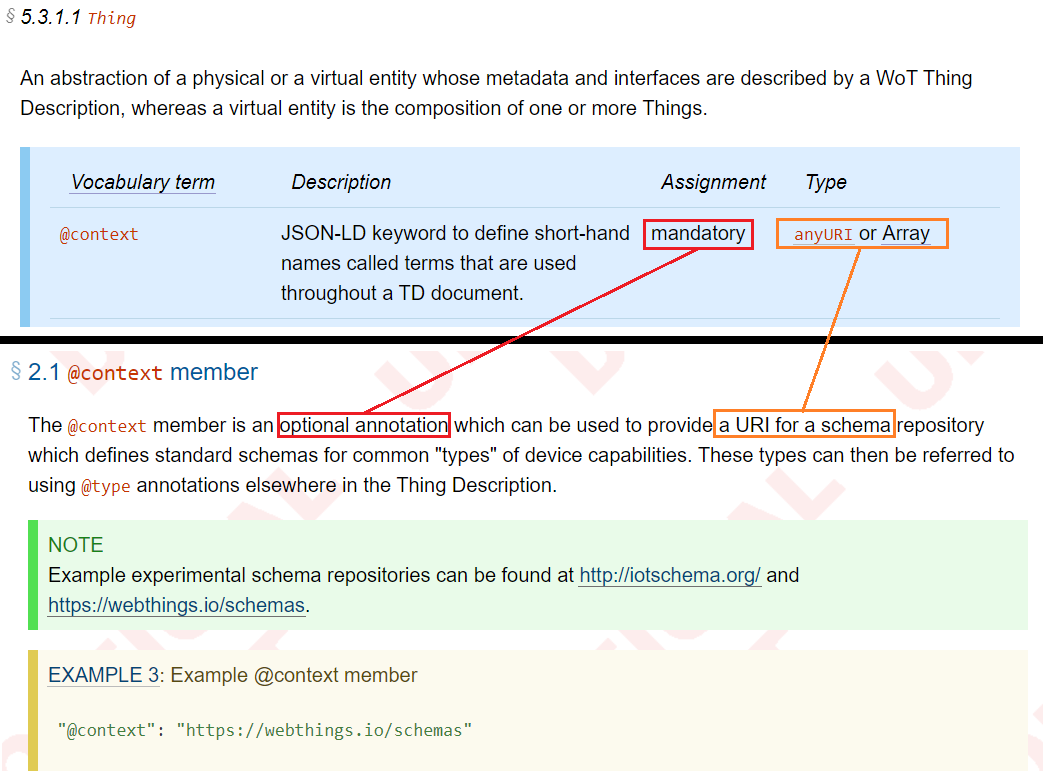
\includegraphics[scale=0.55]{eps/specification-conflict.png}
	\caption{Netto conflitto di specifiche tra \texttt{WebThings.io} e raccomandazioni del W3C.}
	\label{fig:specification-conflict}
\end{figure}

Come da figura \ref{fig:specification-conflict}, entrambe le definizioni collidono, e per puntualizzare il problema, si vuole sottolineare come \href{https://www.w3.org/TR/wot-thing-description/#example-28}{\ul{l'esempio 28}} del \href{https://www.w3.org/TR/wot-thing-description/#semantic-annotations}{\ul{capitolo 7.1}} della descrizione del W3C \textbf{\uline{NON}} sia compatibile con le specifiche di \texttt{WebThings.io}, e che quindi risulterebbe essere completamente illeggibile e inutilizzabile.\\

Rendere impossibile l'uso di ontologie, diverse da quella base, vanifica completamente l'obiettivo di questo progetto, per cui il framework di \texttt{WebThings.io} dev'essere necessariamente scartato. Si sottolinea però che direttamente sul suo repository ufficiale, è stato aperto un ticket di supporto\footnote{Issue 157 - \url{https://github.com/WebThingsIO/api/issues/157}} per richiedere questa funzionalità, che sarà probabilmente integrata in un prossimo futuro.

Come ultima nota, le differenze possono essere trovate sul seguente collegamento: \url{https://github.com/WebThingsIO/wiki/wiki/Mozilla-W3C-Differences}


\subsection{Arena Web Hub}
Framework \cite{arenawh} basato su Node.js contenente esempi di backend e frontend. È un tentativo di standardizzare protocolli differenti, in modo da creare interoperabilità tra essi: infatti, al suo interno, vengono implementati ben tre gateway (Web Hub, Mozilla Gateway e Eclipse Thing Web) che possono essere creati in modo da supportare differenti soluzioni. Le Things vengono create dopo che uno dei tre gateway è stato istanziato, chiamando il metodo \texttt{.produce()}, il quale come l'unico argomento prende in considerazione la Thing Description.\\

Il problema di questa implementazione è simile a quello descritto nella sezione \ref{sec:webthingsio}, trattante del framework di Web Things. Infatti, anche in questa implementazione non è chiaro il supporto per le annotazioni di ontologie diverse da quella standard. L'unica cosa citata nella documentazione è:

\begin{quote}
\textit{Note that the examples include a client-side Web of Things library (see "client/wot.js") with an adaptation layer for different Web of Things platforms. \ul{A \textbf{further library} is planned to make it easy to work with semantic annotations that describe the kinds of things (e.g. a light), their capabilities (e.g. dimmable), and the context in which they reside (e.g. my kitchen)}.}
\end{quote}

Analizzando il codice sorgente\footnote{\url{https://github.com/draggett/arena-webhub/blob/master/webhub.js}}, disponibile su GitHub e visibile in figura \ref{fig:context-overwritten}, è possibile comprendere che il supporto alle annotazioni è infatti \textbf{assente}, ma tecnicamente previsto. Il metodo \texttt{.produce()} sovrascrive tutti i parametri della Thing Description in modo da renderla conforme alle specifiche della libreria stessa, puntando il contesto a quello ufficiale specificato dall'ente W3C. In questo modo, ancora una volta, viene impedita la possibilità di collegarvi ulteriori ontologie e di definire una maggiore conoscenza sulla Thing descritta: infatti, non vi è alcun modo per aggiungerle successivamente e nell'oggetto che definisce la struttura delle Thing vi è una completa assenza del riferimento al contesto.\\

\begin{figure}[h]
	\centering
	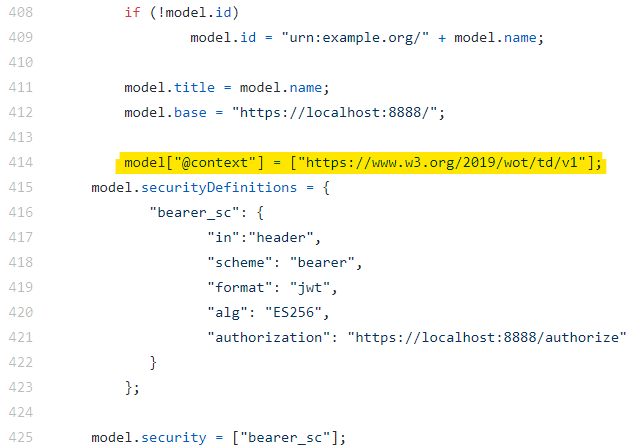
\includegraphics[scale=1]{eps/context_overwritten.png}
	\caption{La libreria implementata sovrascrive alcuni campi della Thing Description con i propri valori, rendendo inutilizzabili le ontologie eventualmente indicante nel contesto. Fonte: \url{https://github.com/draggett/arena-webhub/blob/master/webhub.js}, riga 414}
	\label{fig:context-overwritten}
\end{figure}

Similmente al framework di WebThings, nonostante un vasto supporto alle specifiche di W3C, non vi sono quelle richieste dai requisiti posti. Per questo motivo anche Arena Web Hub dev'essere scartato.


\clearpage
\subsection{ThingWeb.io}
Similmente ai framework trattati, come WebThings.io e Arena Web Hub, anche \textbf{ThingWeb.io} \cite{thingweb} tenta di implementare gli standard raccomandati dal W3C. L'approccio in questo caso parte da un'implementazione Node.js: attraverso di quello si crea un endpoint, il quale poi potrà creare e o vedere Things create. Non vi sono particolari nozioni sul supporto alle ontologie aggiuntive (il problema maggiore delle precedenti soluzioni) e pare avere il supporto per la prototipazione e il lancio di Things virtuali. La documentazione esiste sia sul repository, sia nella pagina ufficiale del progetto.\\

Esistono due concetti importanti per quanto riguarda il framework di ThingWeb.io:
\begin{itemize}
	\item \textbf{Thing \textit{esposta}} è l'effettiva implementazione della Thing, con le sue proprietà, metodi ed eventi. Risulta essere quindi l'effettiva Thing Virtuale che il programmatore può eseguire attraverso un file di lancio\footnote{La questione è spiegata meglio nel capitolo \ref{sec:configuring:wt}}.
	
	\item \textbf{Thing \textit{consumata}} è la Thing che vede l'utilizzatore. Si differenzia dalla prima in quanto può solo interagirvi, e non gestirla completamente: Thing \textit{consumata} è soltanto una facility per interfacciarsi meglio con proprietà e funzioni sottostanti, ma non per gestire, nel verso senso della parola, la Thing virtuale. Si può pensare alla Thing \textit{consumata} come una sorte di interfaccia o un layer che permette di comunicare con l'oggetto.
\end{itemize}

Per scongiurare l'ipotesi del mancato supporto ai diversi contesti, è necessario recarsi più a fondo nella documentazione: le specifiche riguardanti il primo lancio di una Thing all'interno di un Raspberry indicano, ad esempio una Thing Description che, come visibile dalla figura \ref{fig:context-ok-thingweb}, è completa di tutti i campi indicati nella raccomandazione del W3C, compresi alcuni aggiuntivi contesti rispetto a quello base.\\

\begin{figure}[h]
	\centering
	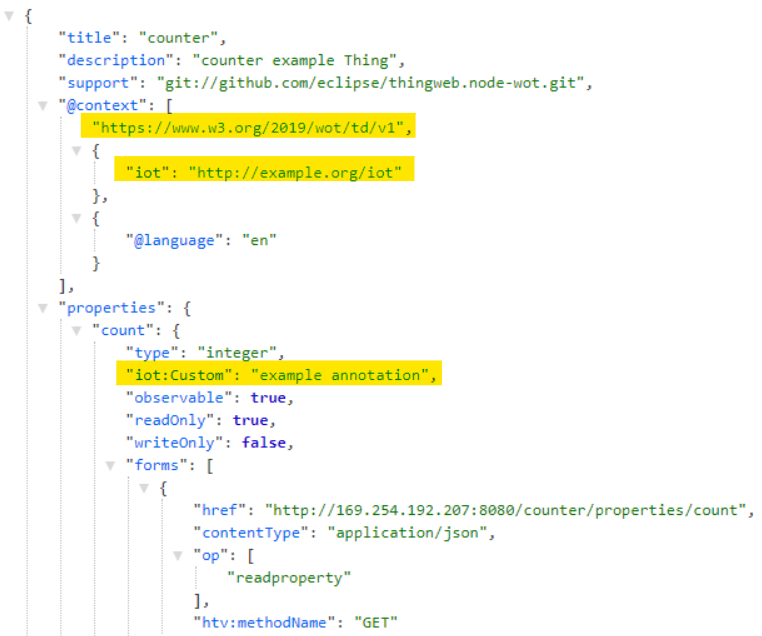
\includegraphics[scale=0.8]{eps/context_ok_thingweb.png}
	\caption{La Thing Description letta da ThingWeb risulta essere completa di tutti i campi. Sono evidenziati i contesti indicati e il loro utilizzo. Fonte: \url{http://www.thingweb.io/hands-on-intro-raspberry.html}}
	\label{fig:context-ok-thingweb}
\end{figure}

Per specificare meglio il supporto alla Thing Description, si può far riferimento al parser della TD, come nella figura \ref{fig:context-ok-thingweb_2}; in esso, quando viene incontrato il campo \texttt{@context} viene effettuato un controllo: in base alla tipologia del dato (stringa o array) vengono istanziate le rispettive risorse.\\

\begin{figure}[h]
	\centering
	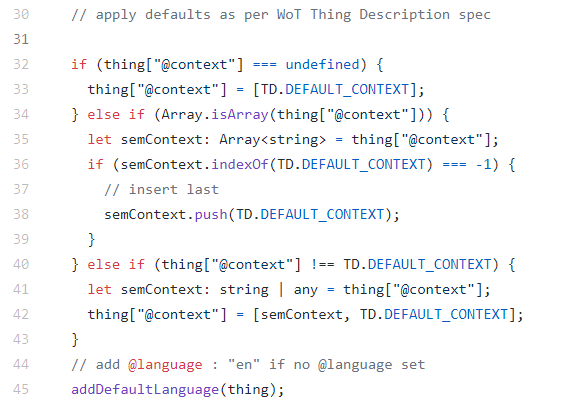
\includegraphics[scale=0.9]{eps/context_ok_thingweb_2.png}
	\caption{Nella riga 35 è chiaramente visibile il supporto a più definizioni di contesti. Fonte: \url{https://github.com/eclipse/thingweb.node-wot/blob/master/packages/td-tools/src/td-parser.ts}}
	\label{fig:context-ok-thingweb_2}
\end{figure}


Al momento, ThingWeb.io risulta essere l'unico framework capace di includere tutte le caratteristiche richieste dal progetto, per risulta essere la scelta definitiva.


%%%%%%%%%%%%%%%%%%%%%%%%%%%%%%%%%%%%%%%%%non numera l'ultima pagina sinistra
\clearpage{\pagestyle{empty}\cleardoublepage}
\chapter{Implementazione delle Web Things}           %crea il capitolo
%%%%%%%%%%%%%%%%%%%%%%%%%%%%%%%%%%%%%%%%%imposta l'intestazione di pagina
\lhead[\fancyplain{}{\bfseries\thepage}]{\fancyplain{}{\bfseries\rightmark}}  

\section{Introduzione}

Si scelgono come attuali strumenti di sviluppo i seguenti programmi:

\begin{itemize}
	\item \textbf{Visual Studio Code}: per la sua versatilità in ambito di programmazione, coprendo quasi tutti i linguaggi meglio conosciuti (anche attraverso l'uso di plugin) risulta essere un'ottima scelta per sviluppare qualsiasi programma. Non presenta particolari aiuti per quanto riguarda suggerimenti intelligenti, ma è sufficientemente ricco di feature per snellire il lavoro.
	
	\item \textbf{Postman}: per mandare i messaggi di test secondo il protocollo REST alle Web Things create, per testare il loro funzionamento e risposte senza necessità di creare applicazioni ad hoc.
\end{itemize}

Si vuole inoltre notare che tutto il successivo capitolo fa riferimento al sistema operativo Windows 10, eseguito su una macchina aventi le caratteristiche espresse nella tabella \ref{tab:pc-spec}.\\

\begin{table}[h]
	\centering
	\begin{tabular}{|l|l|}
		\hline
		\textbf{Component}   & \multicolumn{1}{c|}{\textbf{Name}} \\ \hline
		\textbf{Motherboard} & MSI Z270 M7                        \\ \hline
		\textbf{CPU}         & Intel i7-7700k                     \\ \hline
		\textbf{GPU}         & Gigabyte GTX 1080Ti                \\ \hline
		\textbf{RAM}         & 16GB of Ballistix DDR4 @ 2400MHz           \\ \hline
		\textbf{Disk}        & SSD Samsung Evo Pro 750 1TB                \\ \hline
	\end{tabular}
	\caption{\label{tab:pc-spec} Configurazione del PC in considerazione.}
\end{table}
Gli eventuali codici sorgenti possono essere trovati nella cartella:\\ \texttt{attachments/src}.

\section{Configurazione Framework}
La procedura di configurazione del framework può essere seguita direttamente dalla documentazione del \href{https://github.com/eclipse/thingweb.node-wot/}{repository} \cite{thingweb}. In questa relazione verrà preso in considerazione il metodo descritto come \textit{\quotes{As a standalone application}}.

Si procede dunque all'installazione di dipendenze con il comando:
\begin{lstlisting}[language=bash]
	npm install -g --production windows-build-tools
\end{lstlisting}

Successivamente, viene seguito il tutorial per lanciare il progetto:
\begin{lstlisting}[language=bash]
	# Cloning
	git clone https://github.com/eclipse/thingweb.node-wot
	
	# Installing
	cd .\thingweb.node-wot\
	npm install
	
	# Launching
	npm run build
\end{lstlisting}

Se il framework non dovesse funzionare o presentare problemi all'avvio, si può eseguire anche l'installazione del \texttt{\quotes{CLI Tool}} utilizzando il comando \texttt{npm i @node-wot/cli -g}. 


\section{Configurazione della Web Thing}
\label{sec:configuring:wt}
Una volta verificato che l'applicazione si apre senza maggiori problemi, è possibile procedere con la definizione dell'oggetto che verrà lanciato. Per creare una Thing, a partire dalle Thing Description, è necessario indicare al framework un file \texttt{.js} che contiene il codice permettente all'oggetto esposto di funzionare correttamente, di essere osservato e di reagire ai cambiamenti. A questo punto è utile sottolineare la presenza di uno strumento di WebThing.io, chiamato \href{http://plugfest.thingweb.io/playground/}{\textbf{Playground}}, il quale permette la creazione e la validazione di una Thing Description.\\

Prima di creare un file \textit{launcher} per una Thing, occorre aver installato il pacchetto di NodeJS che permette la lettura di un file. Per ottenerlo, è necessario recarsi nella cartella \texttt{./thingweb.node-wot/} ed eseguire il comando \texttt{npm install fs}.\\

Una volta soddisfatto il soprastante requisito, vi è necessità di spostarsi nella cartella \texttt{/thingweb.node-wot/packages/cli} e crearvi una nuova cartella, chiamata ad esempio \texttt{res}: all'interno di questa verranno collocati i file di lancio e le Thing Description dalle quali creare gli oggetti.\\

Prendendo come esempio sempre la lampadina, è necessario copiare la \texttt{semantic-bulb.json} all'interno di \texttt{/thingweb.node-wot/packages/cli/res} e crearvi un ulteriore file, chiamato ad esempio \texttt{bulb.js}, composto nel seguente modo:
\begin{lstlisting}[language=JavaScript]
	fs = require('fs');
	
	try {
		// Reading file
		fs.readFile("./res/semantic-bulb.json", function(error, data) {
			if (error) {
				console.log("Error when reading")
			} else {
				try {
					// Converting JSON into object
					let obj = JSON.parse(data)
					WoT.produce(obj)
					.then(thing => {
						// Exposing thing to public
						thing.expose()
					})
					.catch(error => {
						console.log(error)
					})
					
				} catch (error) {
					console.log(error)
				}
			}
		})
	} catch (error){
		console.log(error)
	}
\end{lstlisting}

Recandosi successivamente nella cartella \texttt{./thingweb.node-wot/} è possibile lanciare l'applicazione con:

\begin{lstlisting}[language=bash]
	npm start ./res/bulb.js
\end{lstlisting}

È importante sottolineare come l'esplorazione del framework ha riportato già una minuscola criticità: non è possibile infatti passare direttamente la Thing Description al costruttore delle things; è necessario convertirla prima in un oggetto, per poi utilizzarlo. Questo deriva da una feature del framework stesso, prevedente di creare la TD direttamente al suo interno, a partire dall'oggetto passato, non prevedendo che una possibile descrizione potrebbe già esistere. Come però sottolineato, si tratta di una criticità minore, in quanto un oggetto JSON è facilmente deserializzabile e convertibile in un oggetto.\\

Si precisa, inoltre, che esiste un metodo \texttt{.consume()} che parte da una Thing Description per creare un oggetto: risulta però essere un metodo che presuppone l'esistenza della Thing costruita richiamando \texttt{.produce()} e \texttt{.expose()} attraverso il protocollo di \texttt{ThingWeb.io}; \texttt{.consume()} tenterà semplicemente di connettersi e mappare le funzioni e proprietà dell'oggetto remoto creato, in modo da facilitarne l'utilizzo all'interno dello stesso framework.\\

Per permettere una facile configurazione di ulteriori Thing in futuro, si procede alla creazione di un modulo \texttt{common} nel quale raggruppare le funzioni comuni alla creazione delle Things. Il codice di questo file è disponibile negli allegati: \texttt{/attachments/src/common.js}.\\


\section{Test della Web Thing}
Dopo aver lanciato correttamente l'applicazione, e il relativo oggetto, è possibile controllare il suo effettivo funzionamento andandolo a cercare direttamente da un browser: infatti, la Thing sarà esposta all'indirizzo:\\ \texttt{localhost:8080/<thing\_title\_lowercase>}.\\ Ad esempio, nel caso della lampadina, l'indirizzo sarà:\\ \texttt{localhost:8080/bulb}.\\ L'oggetto restituito da questa chiamata risulterà essere proprio la Thing Description passata durante la sua fase di creazione.\\

Per completare il test, è necessario verificare se vi è possibilità di interagire con la Thing in modo virtuale. È necessario, a tal proposito, aggiungere al file di lancio metodi che permettono un corretto \textit{handling} degli eventi che possono capitare. Questa azione è resa disponibile dalle API offerte dal framework: dopo la chiamata del metodo \texttt{.produce()} si può infatti configurare la Thing utilizzando metodi che impostano le callback per la lettura/scrittura delle proprietà e il richiamo delle azioni ed eventi.\\

\subsection{Operazioni preliminari}

Nel caso della \textbf{Thing \textit{esposta}}, vi è un esplicito riferimento all'API contenente tutte le variabili lette dalla Thing Description: infatti, per leggere e/o scrivere e/o osservare le diverse proprietà che espone una Thing è necessario avvalersi di tre metodi messi a disposizione dall'API:
\begin{lstlisting}[language=JavaScript,caption={Metodi per leggere, scrivere o osservare}]
	// Read, write or obsere a property
	thing.readProperty("propertyName").then((data) => {})
	thing.writeProperty("propertyName", value).then(() => {})
	thing.observeProperty("propertyName", (data) => {})
\end{lstlisting}

È comunque comodo tenere un riferimento a variabili locali per delle verifiche interne, dovute ad un cambio in una variabile osservata, o per motivi di sviluppo e/o controllo: esse possono essere usate per poter agevolmente tenere il codice sotto controllo, anche se questo aggiunge una leggera complessità. Le prime righe del codice si riferiscono dunque all'importazione della libreria \texttt{common} e degli attributi che potranno essere trovati nella Thing. Come esempio, si può prendere il codice della lampadina:

\begin{lstlisting}[language=JavaScript,caption={Inizio del codice di \texttt{bulb.js}},label=lst:bulb.js]
const common = require('./common');

// Reference to local variable
let localRef = {
	status: {
		name: "status",
		value: false
	},
	brightness: {
		name: "brightness",
		value: 0
	},
	thing: null
}
\end{lstlisting}

\subsection{Scrittura dei parametri di default}
Si procede quindi al richiamo delle funzionalità comuni, che permettono agevolmente di creare una Thing a partire da un file. Una funzione di \texttt{callback} permetterà di ottenere l'oggetto e consentirà di richiamare i metodi relativi alla Thing \textit{esposta}. È qui che si inizializzano le proprietà della Thing ai valori di default. Si prende come esempio sempre il file della lampadina:

\begin{lstlisting}[language=JavaScript,caption={Creazione della Thing e inizializzazione proprietà read/write in \texttt{bulb.js}}]
common.createThingFromThingDescriptionFile(WoT, "./res/semantic-bulb.json", function(thing) {
	// Save reference to the thing
	localRef.thing = thing
	
	// Set write/read properties
	localRef.thing.writeProperty(localRef.status.name, localRef.status.value)
	localRef.thing.writeProperty(localRef.brightness.name, localRef.brightness.value)
	
	[...]
})
\end{lstlisting}

\subsection{Osservare e reagire al cambiamento di proprietà}
\label{sec:observe_react}
Vi è necessità poi di specificare comportamenti degli oggetti, che potrebbero avere influenze su uno o più parametri. Per questo motivo si predispongono funzioni che \textit{osservano} le proprietà e reagiscono al loro cambiamento. Una lampadina, ad esempio, può avere i seguenti comportamenti:

\begin{itemize}
	\item passaggio da OFF a ON causa il cambiamento della luminosità da un valore a 0 a un valore maggiore di 0. Per comodità, si assume che la lampadina che si accende voglia arrivare alla massina luminosità disponibile (in questo caso 100). La stessa cosa funziona al contrario, passando dallo stato ON allo stato OFF.
	
	\item passaggio da una luminosità maggiore di 0 ad un valore di luminosità pari a 0 causa lo spegnimento della lampadina. La stessa cosa funziona al contrario: quando la luminosità viene impostata a 0, la lampadina verrà spenta.
\end{itemize}

È quindi possibile definire il codice come segue:

\begin{lstlisting}[language=JavaScript,caption={Reagire al cambiamento delle proprietà in \texttt{bulb.js}}, label=lst:Circular]
// Observing status
localRef.thing.observeProperty(localRef.status.name, async(data) => {
	// If status changes, look at the brightness
	let brightness = await localRef.thing.readProperty(localRef.brightness.name)
	
	// If bulb is on
	if (data == true) {
		// Brightness shoud be higher than 0
		if (brightness <= 0) {
			writeProperty(localRef.brightness.name, 100)
		}
	} else {
		// Bulb is off, brightness should be 0
		if (brightness > 0) {
			writeProperty(localRef.brightness.name, 0)
		}
	}
})
[...]
\end{lstlisting}

Un'importante nota va proprio in merito a questa funzione: per quanto comoda, essa viene richiamata ogni tal volta che una proprietà viene cambiata. Non è possibile infatti differenziare un cambiamento proveniente \quotes{\textit{dall'interno}} della Thing da quello proveniente \quotes{\textit{dall'esterno}}. Questo può causare comportamenti indesiderati, soprattutto quando si vanno ad aggiornare più proprietà insieme o quando vi si comincia a creare una dipendenza circolare tra le due proprietà:\\

	\textit{La diminuzione della luminosità a 0 scatta lo spegnimento della lampadina, ma lo spegnimento della lampadina scatta il cambiamento sulla luminosità che dev'essere impostata a 0, che a sua volta scatta lo spegnimento della lampadina che causa l'impostazione della luminosità...}\\
	
Nel caso del codice \ref{lst:Circular} la catena viene spezzata grazie al controllo sul dato in arrivo: se la lampadina è accesa, il suo valore viene modificato solo se la luminosità è minore o uguale a zero, altrimenti non viene effettuata alcuna operazione. Senza questo controllo, la proprietà verrebbe impostata inutilmente, richiamando oltretutto l'\textit{observer} stesso, causando un ciclo infinito.\\ 
	
È necessario notare che \texttt{.writeProperty()} è una funzione creata appositamente che permette la scrittura dei parametri sia locali che remoti della thing. È formata nel seguente modo:

\begin{lstlisting}[language=JavaScript]]
function writeProperty(name, value) {
	// Write object locally
	for (const key of Object.keys(localRef)) {
		if (key == name) {
			localRef[key].value = value
		}
	}
	
	// Wirte object remotely
	return localRef.thing.writeProperty(name, value)
}
\end{lstlisting}


\subsection{Handler delle azioni}
Come ultima cosa, vi è necessità di specificare il comportamento delle azioni che si hanno quando si interagisce con la Thing. Per comodità, si assume che le operazioni non possano essere interrotte, anche se nella realtà è possibile interagire con la Thing in qualsiasi momento, a volte producendo risultati inattesi: ad esempio, attivando il comando \texttt{fade} sulla lampadina è possibile spegnerla e/o accenderla, ma l'esecuzione del comando continuerà finché non raggiungerà il valore impostato, cambiando di conseguenza lo stato in cui essa si trova. Un esempio di come può essere impostata un'azione è nel seguente codice:

\begin{lstlisting}[language=JavaScript,caption={Reagire all'invocazione dell'azione in \texttt{bulb.js}}]
// Toggle reads current status and switch it
localRef.thing.setActionHandler("toggle", async(params) => {
	return localRef.thing.readProperty(localRef.status.name)
	.then((data) => {
		return writeProperty(localRef.status.name, !data)
	})
});
\end{lstlisting}


Vi è da sottolineare che lo standard W3C definisce in maniera molto vaga\footnote{\url{https://github.com/eclipse/thingweb.node-wot/issues/373\#issuecomment-758490819}} quelli che possono essere i modi per interagire con la Thing, per cui ogni framework è sostanzialmente libero di interpretare i vuoti non colmati con soluzioni proprie. Nel caso del protocollo HTTP, utilizzato in questo caso, si può far riferimento alla tabella nel capitolo \textit{8.3.1 Protocol Binding based on HTTP}\footnote{\url{https://w3c.github.io/wot-thing-description/\#http-binding-assertions}} dello standard per la Thing Description, nella quale vi sono specificati soltanto metodi GET, PUT e POST e i relativi utilizzi in base alla proprietà \texttt{op} del campo \texttt{form}.\\

Di conseguenza, \texttt{WebThing.io} non possiede\footnote{\url{https://github.com/eclipse/thingweb.node-wot/issues/373}} al momento una completa definizione delle API REST che si possono usare, ma queste risultano essere deducibili nella maggior parte dei casi: questo purtroppo significa che vi è necessità di spendere tempo per scoprire le possibili combinazioni di chiamate.\\

\subsection{Test di REST API}
Al lato pratico, per controllare la risposta della Thing in merito alle chiamate REST, è possibile utilizzare \textbf{Postman}\footnote{\url{https://www.postman.com/downloads/}} per simulare l'invio e la ricezione dei pacchetti. L'avvio della Thing avviene con il comando:\\
\texttt{npm start ./res/bulb.js}\\

Da qui si performano una serie di operazioni sulla Thing riconosciuta, una volta che quest'ultima risulta essere pienamente operativa. Nel caso della lampadina si possono considerare i seguenti esempi:

\begin{itemize}
	\item \texttt{GET http://localhost:8080/bulb/properties/status}\\
	Ritorna lo stato attuale della Thing in formato di una stringa. Il ritorno dipende dalla proprietà richiesta, ma risulta essere una stringa che rappresenta l'oggetto. Nel caso dello stato risulta essere così formata:
	\begin{lstlisting}[language=JavaScript]
	  true
	\end{lstlisting}
	
	\item \texttt{PUT http://localhost:8080/bulb/properties/status}\\
	Imposta lo stato attuale della Thing. Ha necessità di specificare il \texttt{Content-Type} impostato a \texttt{application/json} e un \texttt{body} nel quale specificare il valore da impostare. Nel caso dell'impostazione dello stato a \texttt{true}, il \texttt{body} risulta essere come segue: 
	\begin{lstlisting}[language=JavaScript]
	  true
	\end{lstlisting}
	La chiamata non ritorna nulla, se non un classico HTTP Status.

	\item \texttt{POST http://localhost:8080/bulb/actions/toggle}\\
	Effettua uno scambio di stato attuale: se la lampadina è accesa, si spegnerà; viceversa, se è spenta si accenderà. Non ha bisogno di specificare alcun contenuto, in quanto è un'azione che non richiede nessun parametro. L'output sarà semplicemente l'HTTP Status ottenuto dalla richiesta.
\end{itemize}

Postman permette l'esportazione della configurazione dell'API: per questo motivo questa è interamente disponibile come allegato nella cartella:\\ \texttt{/attachments/utils/webthings\_postman\_collection.json}.\\

Si sottolinea ancora una volta come i limiti del framework possano rallentare l'intero sviluppo: manca infatti tutta la documentazione relativa al protocollo REST che si può usare per interagire con la Thing. Anche la validazione dei dati in ingresso non è documentata, benchè fattibile: soltanto un'apertura di un \texttt{issue}\footnote{\url{https://github.com/eclipse/thingweb.node-wot/issues/373}} all'interno del repository ha fatto emergere entrambe le cose. Data la possibilità di controllare l'input in arrivo è stata scoperta in uno stadio avanzato del progetto, dove si era fatta ormai l'assunzione dell'assenza di tale feature, si predispone semplicemente un esempio, prendendo la lampadina come oggetto di riferimento e \texttt{fade} come azione per la quale controllare l'input:

\begin{lstlisting}[language=JavaScript]
"input": {
	"type": "object",
	"properties": {
		"level": {"type": "integer", "minimum": 0, "maximum": 100 }
	},
	"required": ["level"]
}
\end{lstlisting}

\begin{lstlisting}[language=JavaScript]
const Ajv = require('ajv');
let ajv = new Ajv();
...

// Fade increment/decrement every 100ms brightness, to give the desired value
localRef.thing.setActionHandler("fade", async(params) => {
	if (!ajv.validate(localRef.thing.getThingDescription().actions.fade.input, params)) {
		return new Error ("Invalid input");
	}
	else {
		fade(params.level);
	}
})
\end{lstlisting}

La validazione avviene tramite la libreria \texttt{ajv}, la quale verifica i parametri di input sulla base di quello che è definito all'interno della Thing Description. Si vuole comunque notare che questa funzionalità risulta essere pseudo-automatica, in quanto è il programmatore che si deve preoccupare di richiamare esplicitamente questa funzionalità, che teoricamente, dovrebbe essere prevista di default nel protocollo.\\

Una volta apportato che è possibile creare, avviare e interagire con una singola Thing semplice, si procede anche all'implementazione delle rimanenti Thing Description e la creazione di oggetti più complessi. Le eventuali note aggiuntive, che introducono novità rispetto ai discorsi affrontati, verranno proposte nel capitolo \ref{sec:other-things}.


\section{Note aggiuntive sulle ulteriori Thing}
\label{sec:other-things}
In questa sezione verranno trattate solo maggiori differenze o dettagli degni di nota sulle things diverse dalla lampadina utilizzata come \quotes{\textit{Thing Esempio}}.


\subsection{Dettagli sulla TV}
A differenza della \textit{lampadina}, la \textbf{TV} possiede la proprietà \texttt{brightness} che può essere impostata a \texttt{0} anche quando la TV è accesa: questo essenzialmente vuol dire che la retroilluminazione del dispositivo è sparita, ma esso continua a far vedere le immagini: questa impostazione potrebbe essere utilizzata di notte. Di conseguenza, l'unico cambiamento che la TV deve osservare è quello relativo al suo stato.\\

Nella \textbf{TV} è possibile portare le proprietà in uno stato inconsistente a causa di una mancanza di controllo sull'effettivo stato di accensione della TV; infatti, se la TV è spenta, non dovrebbe essere possibile impostare il suo volume, canale o luminosità: questo però è permesso. Si presenta quindi la necessità di verificare il valore della proprietà \texttt{status} prima (e/o dopo) aver impostato i parametri:

\begin{itemize}
	\item se si imposta solo un \texttt{observer} (\texttt{.observeProperty()}) sulla proprietà \texttt{status}, ogni handler relativo al cambiamento dello stato sulla TV controllerà l'integrità delle proprietà della Thing soltanto \textbf{dopo} che lo stato sia cambiato. Quindi, spegnendo la TV e facendo passare lo stato da \texttt{true} a \texttt{false}, si impedirà una qualsiasi modifica ai parametri (in quanto la TV spenta non può controllare nessun parametro).
	
	\item se si imposta solo un \texttt{writeHandler} (\texttt{.setPropertyWriteHandler()}) sulla proprietà \texttt{status}, ogni handler relativo al cambiamento dello stato sulla TV controllerà l'integrità delle proprietà della Thing soltanto \textbf{prima} che lo stato cambi. Quindi, accendendo la TV non si farà passare lo stato da \texttt{false} a \texttt{true}, ma si cercherà di modificare i parametri a TV spenta, portando la Thing in uno stato inconsistente (accesa, con volume, canale e luminosità impostate a 0).
	
	\item utilizzando invece l'\texttt{observer} e il \texttt{writeHandler} insieme, teoricamente è possibile coprire entrambi i casi descritti: purtroppo il Framework non facilita il lavoro con proprietà dipendenti tra di loro e il codice (disponibile anche come allegato\footnote{\texttt{attachments/src/tv-not-working.js}}) risulta essere complesso.
\end{itemize}

\begin{lstlisting}[language=JavaScript,caption={Solzuione proposta per la dipendenza tra proprietà della Thing},label=lst:solution]
// Observing status of status property (AFTER write)
localRef.thing.observeProperty(localRef.status.name, async(data) => {
	if (data) {
		// TV passed from OFF to ON: all properties to DEFAULT
	}
})

// Handling write of status property (BEFORE write)
localRef.thing.setPropertyWriteHandler(localRef.status.name, async(data) => {
	if (!data) {
		// TV passed from ON to OFF: all properties to OFF
	}
	return data
})

// Override behavior on writing status for other properties
localRef.thing.setPropertyWriteHandler(localRef.channel.name, async(data) => {
	let isTvOn = await localRef.thing.readProperty(localRef.status.name)
	let currentValue = await localRef.thing.readProperty(propertyName)
	if (isTvOn) {
		return data
	} else {
		return currentValue
	}
})
...
\end{lstlisting}

Per aggravare però la situazione, si vuole notare che la soluzione proposta dal codice \ref{lst:solution} \textbf{non funziona}, in quanto vi è un probabile bug, già segnalato ai creatori del framework\footnote{\url{https://github.com/eclipse/thingweb.node-wot/issues/376}}: il problema deriva dal fatto che cercando di eseguire il metodo \texttt{.readProperty()}, il suo valore sarà ancora impostato su quello precedente, come se l'\texttt{observer} venisse azionato prima di scrivere effettivamente il valore. Nell'esempio del codice \ref{lst:solution}, nella riga 21, la variabile \texttt{isTvOn} risulterà essere quindi \texttt{false}, anche se l'\texttt{observer} ha già rilevato che la TV fosse accesa.\\

Il problema descritto dunque viene affrontato in maniera diversa: anziché utilizzare le proprietà per impostare lo stato della TV, si ridefinisce la Thing Description in modo da prevedere azioni che modificano lo stato. Le proprietà diventano tutte di sola lettura e l'unica ad essere osservata rimane quella relativa allo stato, il quale definisce se la TV si trova in uno stato \quotes{accesa} o \quotes{spenta}. L'allegato \texttt{tv.js} contiene la soluzione  al problema, definendo le specifiche azioni (e relativi controlli) per garantire l'integrità della Thing: anche se minimale, il cambiamento risolve completamente il problema.\\


\begin{lstlisting}[language=JavaScript,caption={Solzuione definitiva per la dipendenza tra proprietà della Thing},label=lst:solution2]
// Set write/read properties
localRef.thing.writeProperty(localRef.status.name, localRef.status.value)
...

// Overwrite behaviour on writing properties: just update them with local data
localRef.thing.setPropertyWriteHandler(localRef.status.name, async(data) => {
	return localRef.status.value
})
localRef.thing.setPropertyWriteHandler(localRef.channel.name, async(data) => {
	return localRef.channel.value
})
...

// Observe status changes
localRef.thing.observeProperty(localRef.status.name, async(data) => {
	if (data) {
		// TV changes its state to ON -> set default values
	} else {
		// TV changes its state to OFF -> set OFF values
	}
})

// Toggle it
localRef.thing.setActionHandler("toggle", async(params) => {
	let status = await localRef.thing.readProperty(localRef.status.name)
	return writeProperty(localRef.status.name, !status)
})

// Change Channel
localRef.thing.setActionHandler("set-channel", async(params) => {
	return checkIfCanWrite(localRef.channel.name, params.channel)
})
\end{lstlisting}

Nel mentre questa soluzione veniva implementata, il framework si era aggiornato e ha corretto il problema, confermando che si trattasse di un richiamo all'observer prima che il valore fosse effettivamente impostato. L'iter della correzione è consultabile nella Issue numero 376 sul repository ufficiale\footnote{\url{https://github.com/eclipse/thingweb.node-wot/issues/376\#issuecomment-762111754}}.

\subsection{Problemi della Tapparella}
Un'assunzione importante per quanto riguarda la \textbf{tapparella} è il fatto che ogni azione effettuata produce un effetto immediato: l'abbassamento o l'innalzamento della Thing non ha il tempo di delay e applica il valore desiderato senza considerare l'eventuale tempo di movimento dovuto a reali parti meccaniche. Questa semplificazione è utile per presentare le potenzialità della Thing, senza andare troppo in dettaglio su come affrontare alcune problematiche intrinseche alla programmazione della Thing stessa.\\

È utile sottolineare che questa cosa vale anche per tutte le altre Things prese in considerazione; la tapparella però risulta quella più evidente, in quanto parti meccaniche in movimento non attuano mai all'istante.



\section{Criticità rilevate nel Framework}
\label{sec:issues}
Nonostante il fatto di aver scelto un framework supportante la Thing Description, essa non vi è pienamente implementata. Esistono infatti alcune problematiche aperte, in sviluppo o da rivedere, che i creatori stanno cercando progressivamente di affrontare. Come per \texttt{WebThings}, dove è stato segnalato un potenziale problema\footnote{\url{https://github.com/WebThingsIO/api/issues/157}} riguardante l'impossibilità di usare più contesti, anche in \texttt{ThingWeb.io} le criticità non sono mancante e hanno causato notevoli ritardi sulla linea di sviluppo predefinita. Si vuole sottolineare che alcuni di questi problemi probabilmente sono stati già citati, ma vengono riportati qui per comodità

\begin{itemize}
	\item \textbf{Creazione di una Thing a partire da Thing Description testuale impossibile}: vi è necessità infatti di passare un oggetto creato appositamente: è quello che poi pensa alla creazione della Thing vera e propria. Esiste quindi questo \quotes{doppio passaggio}, nel quale viene fatto il parsing della Thing Description da un file, poi ne viene creato l'oggetto in Node.js dal quale poi il framework si ricava a sua volta la Thing Description.
	
	\item \textbf{Assenza di dettagliata documentazione}: il framework spesso fa riferimenti alla documentazione generica fornita come linee guida del W3C; generalmente questo non causa problemi con progetti piccoli, ma comincia a diventare complesso da gestire quando le variabili in campo sono molteplici:
		\begin{itemize}
			\item Non vi è una chiara documentazione RESTful, in quanto viene indicato come riferimento soltanto il \href{https://w3c.github.io/wot-thing-description/#http-binding-assertions}{\textit{Protocol Binding Based on HTTP}}\footnote{\url{https://w3c.github.io/wot-thing-description/\#http-binding-assertions}}. Esso specifica comandi differenziando per il tipo di \texttt{op} del \texttt{Form} della Thing Description, ma non menziona ad esempio in nessun modo come viene composto l'URL che permette la lettura e/o scrittura di proprietà. Uno standard ben definito avrebbe sicuramente risparmiato del tempo in fase di esplorazione e creazione delle Things.
			
			\item Esiste una piccola confusione per quanto riguarda variabili locali e della Thing Stessa: è più indicato infatti usare le seconde, asincrone, direttamente collegate alla Thing Stessa, piuttosto che quelle locali, come da alcuni esempi\footnote{\url{https://github.com/eclipse/thingweb.node-wot/blob/master/examples/testthing/testthing.js}} che sono reperibili nel \textit{repository} ufficiale. Dall'altro canto, in una delle discussioni aperte nelle Issue, è emerso che nel prossimo futuro verrà consigliato l'approcio considerante le variabili \textit{locali}\footnote{\url{https://github.com/eclipse/thingweb.node-wot/issues/376\#issuecomment-762111754}}.
			
				\textit{Note: in the upcoming API does not any longer have built-in handlers for writeProperty and this problem goes away. Anyhow, fixing the current state makes sense to me.}
			
			\item non vi è una documentazione ufficiale per quanto riguarda la validazione del \texttt{form} soltanto un'apertura di un issue\footnote{\url{https://github.com/eclipse/thingweb.node-wot/issues/375\#issuecomment-759588714}} ha fatto emergere una libreria esterna (\texttt{ajv}) attraverso la quale è possibile validare i dati in ingresso.
			
			\item non vi è alcun standard per quanto riguarda la formattazione dei dati: per impostare lo stato di una lampadina a \texttt{true} occorre semplicemente mandare un messaggio \texttt{PUT} sulla proprietà dello stato con il \texttt{body} avente soltanto la parola "\texttt{true}" al suo interno. La formattazione così ottenuta potrebbe risultare illeggibile e portare a problemi relativi ad oggetti più complessi. Una parziale soluzione è data dalla validazione dei dati attraverso la libreria \texttt{ajv}.
			
			\item come sottolineato dalla \textbf{TV}, è possibile strutturare la Thing pensandola in maniera diversa, in quanto è possibile impostare lo stato direttamente come proprietà e/o come azione, dipendentemente da cosa dichiara la Thing Description. Essendovi però diverse problematiche relative a dipendenze tra proprietà sarebbe più lecito indicare nella documentazione delle linee guida per la definizione di oggetti con tali caratteristiche, senza basarsi solo su esempi relativamente semplici.
		\end{itemize}
	
	\item \textbf{Esempi di codice non sufficienti}: quelli forniti sono per la maggior parte piccoli o contrastanti; mentre in uno la Thing utilizza solo variabili interne al codice, in un altro fa uso soltanto di metodi come \texttt{thing.readProperty()} asincroni che cambiano completamente la struttura del programma. Inoltre, non è specificato in nessun modo che non vi è un \texttt{binding} tra parametri \quotes{locali} e quelli della thing, portando ad una errata conclusione sul fatto di poter utilizzare solo i primi per definirla completamente.
\end{itemize}

Le seguenti \textit{issue} segnalate sui relativi \textit{repository} non devono essere prese necessariamente come una nota negativa: si vuole notare infatti la volontà sia dell'utilizzo di queste piattaforme, sia al contribuire alla loro crescita segnalando potenziali problemi, rischi e mancanze. È da sottolineare però l'impegno della comunità a risolvere questi problemi: infatti, essa continua a mantenere e sviluppare nuove funzionalità di questo framework. Le \textit{issues} aperte  hanno ricevuto un'immediata risposta e il messaggio subliminale mandato da chi rispondeva tramandava una forte volontà di risolvere le problematiche poste.

È comunque un'importante fattore che ha segnato notevolmente il progetto, per cui si preferiscono esplicitamente elencare le \textit{issues} aperte:

\begin{itemize}
	\item \textbf{[WebThings]} Issue 157\\
	\url{https://github.com/WebThingsIO/api/issues/157}\\
	Assenza di supporto per più \texttt{@context}
	
	\item \textbf{[ThingWeb.io]} Issue 373\\
	\url{https://github.com/eclipse/thingweb.node-wot/issues/373}\\
	Assenza di documentazione di REST API
	
	\item \textbf{[ThingWeb.io]} Issue 375\\
	\url{https://github.com/eclipse/thingweb.node-wot/issues/375}\\
	Validazione dei dati attraverso il \texttt{form} della Thing Description
	
	\item \textbf{[ThingWeb.io]} Issue 376\\
	\url{https://github.com/eclipse/thingweb.node-wot/issues/376}\\
	\texttt{observeProperty()} ha un valore diverso da \texttt{readProperty()}\\
\end{itemize}




\section{Criticità nell'implementazione delle Things}
La maggior parte delle cose qui elencate risulta essere frutto di compromesso tra funzionalità e API del framework usato parzialmente disponibili e/o scarsamente documentate. Si tratta perlopiù di piccoli accorgimenti che avrebbero portato via del tempo e non avrebbero incluso nel progetto una significativa quantità e qualità di informazioni.

\begin{itemize}
	\item Nelle Things è possibile trovare una semplificazione per quanto riguarda gli eventi che durano nel tempo: ad esempio, nella lampadina, chiamando la funzione \texttt{fade} ed eseguendo successivamente uno spegnimento della stessa, l'azione di \texttt{fade} non si fermerà e vorrà comunque raggiungere il proprio valore (di default 60). L'intensità luminosa quindi verrà impostata a 0 a causa dello spegnimento, ma poi continuerà a crescere fino al valore stabilito dalla funzione di \texttt{fade}. La correzione richiede un controllo su chi esegue la scrittura sulla proprietà \texttt{brightness}: se è l'utente ad aggiornarla, l'azione deve fermarsi; se è la lampadina stessa, l'azione deve continuare;  
	come specificato però nel capitolo \ref{sec:observe_react}, differenziare tra azione \textit{interna} ed \textit{esterna} è al momento impossibile.
	
	\item Non vi è un controllo esplicito e intrinseco sulla correttezza dei parametri passati. È quindi erroneamente possibile, ad esempio, impostare la luminosità di una lampadina come una stringa (\texttt{"esempio"}), senza che la Thing se ne accorga. Come già sottolineato più volte però, questo è risolvibile applicando manualmente il controllo con la libreria \texttt{ajv}.
	
	\item Non vi sono criteri di sicurezza implementati, anche se è possibile definirli all'interno della Thing Description stessa. Questo è solo per semplificare il lavoro e dimostrare le potenzialità del framework e della Thing Description: per coprire ogni aspetto non vi sono tempo e risorse necessarie all'esplorazione e documentazione.
	
	\item Per ognuna delle Thing viene supposto un valore di \textit{default} che si imposta automaticamente ad ogni accensione e spegnimento del dispositivo. Generalmente, si tratta di valori nulli, booleani \texttt{false} e interi pari a 0 quando le Things risultano essere spente, mentre valori di default predefiniti quando vengono accese. Una miglioria delle stesse potrebbe essere quella di includere un file di configurazione che salva automaticamente l'ultima impostazione dell'utente; di conseguenza alla riaccensione del dispositivo i valori verrebbero presi da questo file (e non impostati \textit{di default}).
	
	\item Come scritto nel capitolo \ref{sec:adding-semantic}, la costruzione delle Thing ha fatto emergere la necessità di sviluppare e/o estendere ontologie, in quanto vi sono alcuni aspetti intrinseci delle cose che potrebbero essere rappresentate con maggior dettaglio, ma sempre per motivi di mancanza di tempo e risorse non è possibile coprire ogni aspetto riguardante la Thing Description: il campo della semantica è troppo vasto per poterlo coprire all'interno di un progetto che già mira ad esplorare diversi aspetti.
\end{itemize} 


\section{Endpoint delle Things}
Partendo dalla cartella \texttt{./thingweb.node-wot/} il lancio delle Things avviene tramite un unico comando:

\begin{lstlisting}[language=bash]
	npm start ./res/bulb.js ./res/tv.js ./res/shutter.js ./res/fan.js
\end{lstlisting}

Le Thing così create vengono automaticamente istanziate e inserite all'interno di un endpoint, disponibile sull'indirizzo locale e porta 8080. Anche con un semplice browser è possibile verificarne il funzionamento, in quanto interrogato dovrebbe restituire i collegamenti a tutte le Thing attualmente presenti all'interno del sistema. Dato che presenta la caratteristica di esporre direttamente i dati delle Thing, esso verrà utilizzato come endpoint dell'applicazione in sviluppo.\\


%%%%%%%%%%%%%%%%%%%%%%%%%%%%%%%%%%%%%%%%%non numera l'ultima pagina sinistra
\clearpage{\pagestyle{empty}\cleardoublepage}
\chapter{L'uso della conoscenza}           %crea il capitolo
%%%%%%%%%%%%%%%%%%%%%%%%%%%%%%%%%%%%%%%%%imposta l'intestazione di pagina
\lhead[\fancyplain{}{\bfseries\thepage}]{\fancyplain{}{\bfseries\rightmark}}  

\section{Configurazione}
La conoscenza delle Things è intrinseca alla Thing Descritpion legata agli oggetti creati. In una visione completamente Pervasive, ogni Thing nuova aggiunta al sistema fa in modo da pubblicare, in qualche modo, la sua descrizione, in modo tale da contribuire alla creazione di un'unica descrizione più grande, riguardante l'environment nel quale è attualmente situata. Esiste quindi una raccolta completa di tutte le Thing Descriptions che può essere trattata come se fosse una descrizione (anche semantica) della stanza della quale si vogliono conoscere le Things e le loro relative proprietà e/o azioni.\\

\subsection{Conoscenza unificata}
Per motivi di semplicità si suppone che questa conoscenza sia già a disposizione, considerando le Thing Description create. Per usufruirne a pieno, però, occorrono alcuni semplici passaggi.\\

\begin{enumerate}
	\item La conoscenza non è pronta ad essere sfruttata da interpreti, infatti dev'essere opportunamente convertita in schemi come OWL o RDF: per questo scopo si utilizza un Tool Online chiamato \textbf{RDF Translator} \cite{rdf-translator}, il quale applica automaticamente la conversione JSON-LD in uno dei formati supportati. Nel caso specifico, si inserisce come formato input \texttt{JSON-LD} e come formato output \texttt{Pretty RDF/XML}. I singoli 4 file ottenuti vengono presi in formato \texttt{RAW} e salvati localmente. I file in questione sono disponibile come allegato nella cartella:
	\texttt{/attachments/td/RDF}
	
	\item Esplorando i singoli file, è possibile notare che ognuno di essi definisce ogni Thing, racchiusa all'interno di tag \texttt{XML}: si crea quindi un unico file contenente le 4 descrizioni, accomunate semplicemente dalle prime righe di ogni file, definente le ontologie caratterizzanti la descrizione. Il file in questione è disponibile anche come allegato:	
	\texttt{/attachments/td/RDF/unified.xml}
	
	\item Avendo a disposizione il repository su GitHub\footnote{https://github.com/Martinocom/pervasive-semantic-exam}, si utilizza quest'ultimo come lo storage della conoscenza online, per simulare un endpoint al quale dover fare richieste in remoto.
\end{enumerate}

\subsection{Protégé}
Senza un progetto sottostante, realizzato successivamente, si vuole prima di tutto mostrare le potenzialità della semantica. Per poter interrogare la conoscenza il linguaggio utilizzato sarà \textit{SPARQL} \cite{sparql}: il suo costrutto simile a un classico \textit{SQL} facilita il suo utilizzo. Rimandando per le definizioni più precise al sito ufficiale, si vuole sottolineare subito che il programma utilizzato per simulare le richieste risulta essere Protégé \cite{protege}.\\

L'import della conoscenza avviene tramite il menu contestuale, attraverso l'azionamento di \textit{File > Open from URL...}, specificando poi il link verso il file precedentemente creato (\textit{unified.xml}). All'interno di essa vi sono già presenti tutti i prefissi necessari per le interrogazioni.


\section{Utilizzo}

\subsection{SPARQL}
Si precisa che per ogni interrogazione eseguita, vengono prima di tutto specificati alcuni prefissi, elencati di seguito:

\begin{lstlisting}[language=XML]
	PREFIX rdf: <http://www.w3.org/1999/02/22-rdf-syntax-ns\#>
	PREFIX owl: <http://www.w3.org/2002/07/owl\#>
	PREFIX rdfs: <http://www.w3.org/2000/01/rdf-schema\#>
	PREFIX xsd: <http://www.w3.org/2001/XMLSchema\#>
	PREFIX saref: <https://w3id.org/saref\#>
	PREFIX td: <https://www.w3.org/2019/wot/td/v1>
\end{lstlisting}

Per interrogare la conoscenza, vengono proposti esempi più significativi, rappresentati soltanto la cima delle potenzialità di questo linguaggio. 

\begin{itemize}
	\item Ottenimento di tutte le proprietà all'interno del modello:
	\begin{lstlisting}[language=XML]
	SELECT DISTINCT ?property WHERE {
		?s ?property ?o .
	}
	\end{lstlisting}

	\item Ottenimento di tutte le classi all'interno del modello:
	\begin{lstlisting}[language=XML]
	SELECT ?s ?p ?o WHERE {
		?s rdf:type owl:Class .
	}
	\end{lstlisting}

	\item Ottenimento di tutte le funzionalità di tutte le Things:
	\begin{lstlisting}[language=XML]
	SELECT ?s ?p ?o WHERE {
		?s saref:hasFunction ?o .
	}
	\end{lstlisting}

	\item Ottenimento di tutte le Thing che possono illuminare:
	\begin{lstlisting}[language=XML]
	SELECT ?s WHERE {
		?s saref:accomplishes "saref:Lighting" .
	}
	\end{lstlisting}

	\item Ottenimento di tutte le Thing che sono degli \textit{saref:Actuator}
	\begin{lstlisting}[language=XML]
	SELECT ?s WHERE { 
		?s ?p saref:Actuator
	}
	\end{lstlisting}

	\item Ottenimento di azioni di una lampadina (\textit{bulb}) che sono di tipo \textit{OpenCloseFunction} e che permettono l'azionamento del comando \textit{open}.
	\begin{lstlisting}[language=XML]
    SELECT ?thing ?actionName ?command ?actionType
	WHERE {
		?thing saref:hasFunction ?actionName .
		?actionName saref:hasCommand ?command .
		?actionName rdf:type ?actionType .
		FILTER REGEX(str(?actionType), "OpenCloseFunction", "i") .
		FILTER REGEX(str(?command), "open", "i") .
		FILTER REGEX(str(?thing), "bulb", "i") .
	}
	\end{lstlisting}

	\item Ottenimento di tutte le proprietà del ventilatore (\textit{fan}) che possono impostare lo stato.
	\begin{lstlisting}[language=XML]
    SELECT ?s ?o ?c
	WHERE {
		?s saref:hasState ?o .
		?o rdf:type ?c .
		FILTER REGEX(str(?c), "MultiLevelState", "i") .
		FILTER REGEX(str(?s), "fan", "i") .
	}
	\end{lstlisting}
\end{itemize}


\subsection{SWRL}
La potenzialità di poter includere delle regole all'interno della conoscenza rende possibile ad un potenziale \textit{reasoner} di inferire ulteriore conoscenza, a partire da quella base. Potenzialmente quindi, è possibile definire delle regole attraverso le quali, anche se non esplicitamente indicato, è possibile dedurre la tipologia o le azioni di una Thing in base a quello che essa riesce a fare. L'uso di ontologie note permette di semplificare questo procedimento, in quanto vi possono esistere dei pattern che caratterizzano un gruppo di specifici device, i quali hanno, ad esempio, proprietà o azioni comuni. Tutto questo è possibile grazie a SWRL \cite{swrl}, che esprime i legami che esistono tra classi. Alcuni esempi teorici, che utilizzano come riferimento l'ontologia SAREF, possono essere trovati di seguito:

\clearpage

\begin{itemize}
	\item {\textit{Un qualsiasi oggetto che altera la luminosità e che ha uno stato e possiede due azioni di regolazione del suo stato è un \textit{saref:LightingDevice}}}
	\begin{lstlisting}
	saref1:hasState(?d, saref1:OnOffState) ^ 
	saref1:hasFunction(?d, saref:LevelControlFunction) ^ 
	saref1:hasFunction(?d, saref:OnOffFunction) ^
	saref1:accomplishes(?d, saref:Lighting) -> saref1:LightingDevice(?d)
	\end{lstlisting}

	\item {\textit{Un qualsiasi oggetto che possiede la funzionalità \textit{toggle}, possiede sicuramente una proprietà che ne definisce lo stato}}
	\begin{lstlisting}
	saref1:hasFunction(?d, saref:Toggle) -> saref1:hasState(?d, saref:State)
	\end{lstlisting}
\end{itemize}

Si sottolinea come con semplici dichiarazioni sia possibile definire conoscenza che prima non vi era presente. Considerando però la molteplicità di risorse definibili in questo modo, e la necessità di concentrarsi più sulle potenzialità che sulla realizzazione della conoscenza nell'ambito, si ritiene opportuno proseguire sulla strada delimitata dal progetto e non approfondire ulteriormente l'argomento. Si vuole comunque lasciare questo spunto come fonte di ulteriore motivazione per cui l'uso della semantica risulta essere enormemente utile anche nell'ambito di WoT.



%%%%%%%%%%%%%%%%%%%%%%%%%%%%%%%%%%%%%%%%%non numera l'ultima pagina sinistra
\clearpage{\pagestyle{empty}\cleardoublepage}
\chapter{Agenti, WoT e Semantica}           %crea il capitolo
%%%%%%%%%%%%%%%%%%%%%%%%%%%%%%%%%%%%%%%%%imposta l'intestazione di pagina
\lhead[\fancyplain{}{\bfseries\thepage}]{\fancyplain{}{\bfseries\rightmark}}  

\section{Perchè Agenti?}
Il sistema ad Agenti nasce per diverse esigenze, che comprendono diversi ambiti. Il principale motivo per cui è più utile pensare ad un sistema eterogeneo organizzandolo più in modo Agent-Oriented è la completa indipendenza dell'esecuzione di ogni singolo componente (Agenti incapsulano anche il controllo, il ciclo di vita di uno è indipendente dagli altri) e la possibilità di astrarre a livello ancora più elevato rispetto alla OOP. Inoltre il modello ad Agenti offre la possibilità di rappresentare ancor da più vicino il mondo reale che ci circonda, in quanto questo è effettivamente formato da diverse entità (umani e/o macchine) che interagiscono continuamente tra di loro.\\

Parlando quindi soltanto in termini di praticità e progettazione, è già molto più facile per un programmatore immaginarsi le Web Things come delle entità immerse dentro una stanza (Environment) che interagiscono tra di loro ed, eventualmente, hanno una gerarchia tale da permettere un pieno controllo delle azioni che vengono svolte all'interno dell'ambiente. Immaginando dunque di dover realizzare un sistema WoT, si pone davanti ad un problema di organizzazione delle Web Things e della comunicazione tra di loro. Davanti ad uno studio di una Smart Room, si presuppone di avere alcuni oggetti Smart con le loro caratteristiche, con le quali l'utente può interagire. Dovendo pensare ad un modello ad alto livello, si può a produrre lo schema, visibile nella figura \ref{fig:use-case-diagram-high}, come illustrazione di ciò che potrebbe avvenire dentro questo ambiente.\\

\begin{figure}[h]
	\centering
	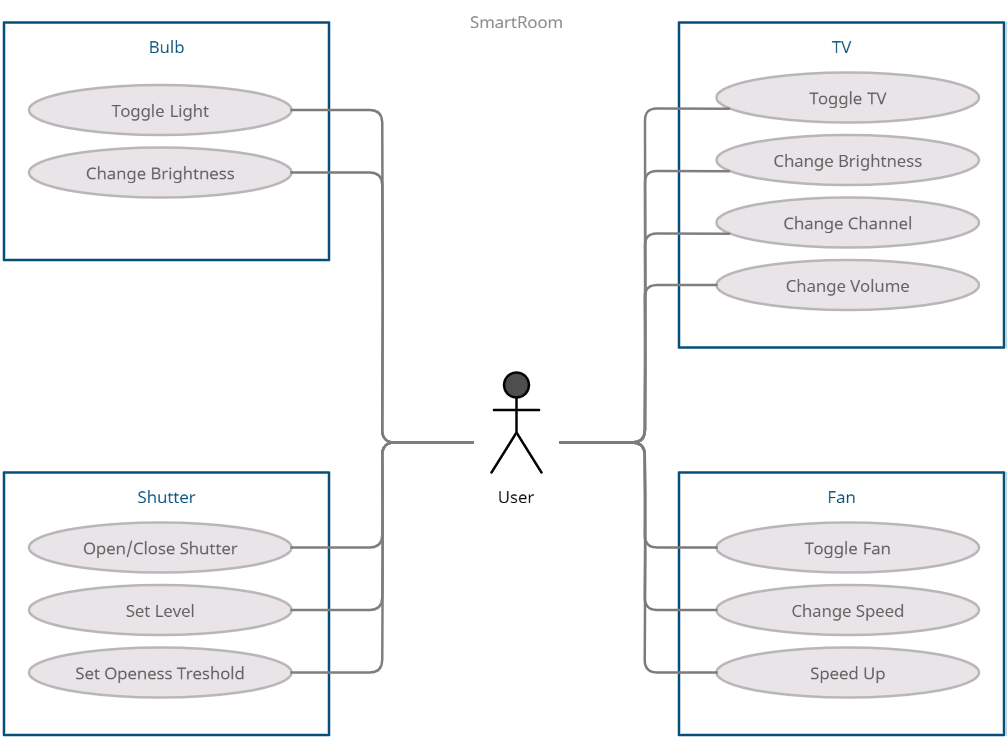
\includegraphics[scale=0.5]{eps/use-case-high-agent-simple.png}
	\caption{Rappresentazione ad alto livello di una Smart Room e suoi oggetti.}
	\label{fig:use-case-diagram-high}
\end{figure}

Pensandolo nel modo classico, ognuno dei sistemi rappresentati dovrebbe avere una classe che lo definisce, metodi con i quali posso interagire e caratteristiche specifiche per ogni singolo oggetto, eventualmente derivate. Una progettazione di classi rappresentative però non è l'unico step da eseguire, in quanto, successivamente, ognuna di esser dovrebbe esporre protocolli di comunicazione, dipendenti dall'oggetto in atto. Vi è poi necessità di un sistema che collezioni le istanze delle classi, e richiami opportunamente gli oggetti con il quale l'utente vuole interagire.\\

Si può volgere di conseguenza lo sguardo alla descrizione presente sopra e calarla all'interno di un ambiente Agent-Oriented, dove i vari oggetti Smart sono Agenti/Artefatti. In questo modo si può astrarre ancor di più la progettazione, non calandosi direttamente alla rappresentazione tramite classi, ma proprio come entità del mondo vero calate quasi direttamente in quello ad Agenti. Come citato in \quotes{\textit{Agent-based modeling: Methods and techniques for simulating human systems}} \cite{abm}, la modellazione ad agenti possiede tre benefici:

\begin{itemize}
	\itemsep0em 
	\item cattura meglio i fenomeni che avvengono tra entità,
	\item fornisce una descrizione più naturale del sistema,
	\item risulta essere più flessibile.
\end{itemize}

È quindi di estrema semplicità immaginarsi un sistema Agent-Oriented ad alto livello, incentrato sulle interazioni Utene-Oggetti. Calandosi nel mondo JaCaMo, infatti, per ogni Smart Thing si può definire il suo Artefatto; successivamente, un agente addetto all'osservazione di questi potrà monitorare le preferenze dell'utente e interagire anche in modo autonomo con l'ambiente, per soddisfare eventuali esigenze. L'utente sarà facilitato nell'interazione con il sistema attraverso un'interfaccia grafica, potendo immettere comandi da eseguire.

\begin{figure}[h]
	\centering
	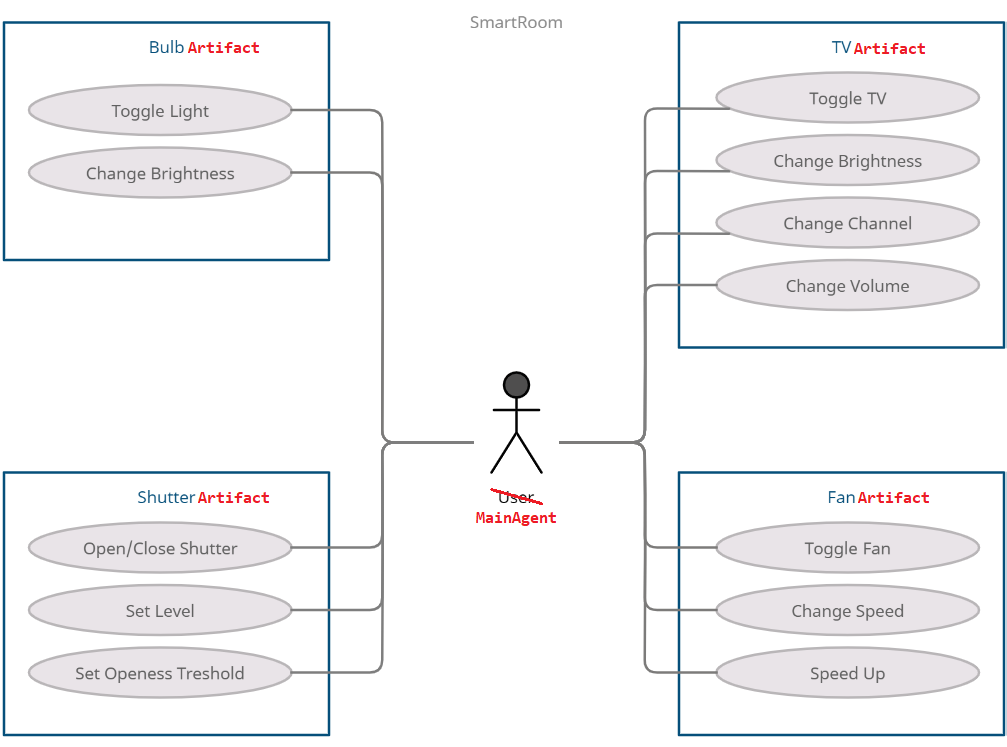
\includegraphics[scale=0.5]{eps/use-case-jacamo.png}
	\caption{Esempio di astrazione della realtà Agent-Based secondo il framework JaCaMo.}
	\label{fig:use-case-diagram-high-agent}
\end{figure}

Come si può notare dalla figura \ref{fig:use-case-diagram-high-agent}, la progettazione di un sistema ad Agenti è direttamente mappata nel mondo reale. Ciò, come sottolineato in precedenza, porta ad un netto vantaggio sull'astrazione del sistema e sulla sua futura implementazione, in quanto nella visione Agent-Oriented tutto viene completamente incapsulato all'interno delle singole entità. Ovviamente, questa non risulta essere una completa progettazione: lo schema vuole dimostrare soltanto il diretto vantaggio che si ha sopra una progettazione classica ad Oggetti.\\

L'utilizzo del modello ad Agenti, inoltre, non riguarda soltanto semplici contesti come la Smart Room: vi sono infatti presenti studi che spaziano argomenti riguardanti sistemi di evacuazione \cite{evacuation} o addirittura l'osservazione delle api \cite{bee}.

\section{Perchè Semantica con Agenti?}
Come affrontato nel capitolo \ref{sec:semantic}, è importante poter specificare non solo una semplice descrizione, ma anche una parte semantica a quello che risulta essere l'oggetto osservato. Calandosi più nel dettaglio dell'implementazione, è possibile infatti immaginarsi un Agente capace di ragionare su un obiettivo imposto (illuminare la stanza), capendo autonomamente con quali oggetti può interagire per conseguire quell'obiettivo. La semantica sblocca inoltre ulteriori aree di sviluppo, quali prevedono del reasoning per scoprire dinamicamente non solo nuovi oggetti, ma funzionalità legate ad essi che, ad esempio, se combinanti in un certo modo, possono raggiungere un obiettivo che non era possibile soddisfare in principio. Utilizzare Agenti per questi scopi risulta essere naturale, in quanto questo è intrinsecamente scritto nella natura BDI, dove a partire da una conoscenza si vogliono ottenere dei risultati, motivando così ancor di più la scelta degli Agenti come piattaforma di progetto finale.


\section{BDI e Web Things}
Il modello BDI si basa sui concetti di \textit{\textbf{b}eliefs}, \textit{\textbf{d}esires} e \textit{\textbf{i}ntentions}. Vi è necessità di analisi per quanto riguarda le seguenti affermazioni e quali sono i vantaggi (e/o svantaggi) di utilizzare questa metodologia per lo sviluppo di un sistema WoT.\\

Come citato da \textit{\quotes{MATCH: MultiAgent-based Tactful CooperationScheme for Heterogeneous IoT Devices}} \cite{masiot}, utilizzare agenti può determinare una semplificazione della gestione per quanto riguarda l'eterogeneità delle cose naturalmente presenti in un ambiente, dati diversi contesti nei quali un sistema ad Agenti può essere applicato. Bisogna però saper specificare con criteri rigorosi i comportamenti che le cose debbano avere, in modo da garantire sia la sicurezza delle persone che il risultato atteso, portando ad una collaborazione (e non competizione) tra le cose che si hanno a disposizione.\\

Come descritto in \textit{\quotes{Building Cyber-Physical Systems - A Smart Building Use Case}} \cite{smartbuilding}, anche una semplice casa possiede diverse sfide, sia per quanto riguardo l'eterogeneità delle cose che la complessità delle azioni da compiere. Vi sono infatti diversi strati di interoperabilità che possono esistere. Dall'altra parte, seppur non citando direttamente, l'articolo fa anche riferimento all'uso di ontologie (o comunque tecnologie standard) per quando riguarda il layer della descrizione degli oggetti e del loro stato, ricadendo perfettamente nell'ambito della Thing Description.\\

La possibilità di strutturare funzionalità definendo dei piani d'azione risulta essere comoda non solo per catturare meglio la natura asincrona degli eventi (ad esempio, l'utente che interagisce con un terminale che cambia lo stato delle cose), ma anche l'ideazione stessa del processo di sviluppo. Infatti, è \quotes{naturalmente umano} immaginarsi una serie di azioni da compiere, quando si vuole raggiungere un obiettivo: cosa rispecchiata quasi perfettamente nella modellazione ad Agenti.\\

Inoltre, l'utilizzo del sistema ad Agenti offre nuove potenziali applicazioni per quanto riguarda il \textit{reasoning} sull'ambiente osservato: essendo un'entità proattiva-reattiva, l'Agente, se configurato, può in autonomia eseguire azioni per garantire il massimo comfort e la sicurezza agli utilizzatori che ne usufruiscono, interagendo con tutte le Thing che esso può avere a disposizione, capendone eventualmente man mano le potenzialità. È di indubbia importanza sottolineare che sia giusto definire come \quotes{dispositivo illuminante} una qualsiasi Thing che abbia la capacità di cambiare la luminosità di un ambiente, ma che tale definizione potrebbe portare ad un eventuale fraintendimento del vero scopo di quel Device: è infatti assurdo pensare che per illuminare la stanza si debba accendere una TV oppure una lavatrice, soltanto perchè al loro interno esistono dispositivi in grado di produrre luce.\\

Uno spunto per quanto riguarda l'approfondimento sull'applicazione più estensivo del modello BDI è invece quello legato all'integrazione della conoscenza della Thing Description (o la sua corrispettiva versione RDF/XML) \textbf{direttamente} all'interno dei \textit{belief} dell'Agente, sfruttandola in maniera completamente indipendente da un endpoint ed eventuali \textit{reasoner} esterni. Non solo; è infatti possibile pensare, come definito nel capitolo \ref{sec:thing_status}, di avere non solo la parte statica, ma anche quella dinamica delle cose, osservando direttamente i parametri delle Things e interagendo con loro.\\

Tutto questo giustifica l'uso degli Agenti: anche per il semplice motivo di essere abilitante per una serie di funzionalità che con una classica programmazione risulterebbero complesse da progettare e da gestire.\\

\clearpage
\subsection{Ordine ed esecuzione delle azioni}
La capacità degli Agenti ad essere predisposti a interagire tra di loro, anche autonomamente, risulta essere un netto (teorico) vantaggio per quanto riguarda l'implementazione di un sistema Smart: il modello a scambio di messaggi abbraccia completamente la natura asincrona negli eventi che possono capitare all'interno di un ambiente, ma bisogna essere precisi nello specifico sulle priorità dei messaggi in arrivo. Di default, infatti, non vi è implementato un modo per ordinare i messaggi che un Agente si vede arrivare.\\

Per questo motivo vi sono presenti strumenti per gestire la priorità delle azioni: è necessario però porre attenzione a non disporre i controlli all'interno dell'Agente stesso, ma nella parte relativa alla ricezione e gestione messaggi. L'agente, infatti, deve poter eseguire le proprie intenzioni anche in assenza di alcune conoscenze, se questo vi è permesso: la belief (iniziale e imparata) è esattamente il motivo per il quale ciò è possibile, se ovviamente l'entità è capace di valutare con accuratezza la situazione dell'ambiente in cui si trova.\\

Non bisogna però intendere questo come una carta bianca per gli Agenti ad eseguire azioni che ritengono giuste: è compito del programmatore a rendere le singole entità sicure, in modo da poter interrompere operazioni, anche critiche, nel caso di uno o più fallimenti. Gli Agenti sono infatti liberi di creare nuovi Agenti (o nel caso di JaCaMo, anche Artefatti) e di eliminarli a dovere: quest'ultima viene vista come un'operazione importante, in quanto l'eliminazione di una entità provoca automaticamente la distruzione di tutte quelle sottostanti nella sua gerarchia.\\

Sempre in caso di JaCaMo, è importante sottolineare che sia l'esecuzione di operazioni all'interno dello scope dell'Agente stesso (quindi le cosiddette \textit{Internal Functions}) che quelle legate ad un Artefatto, risultano essere bloccanti fino a quando non finiscono il loro ciclo di esecuzione. Eseguendo quindi una potenziale lunga operazione, come lettura di un file o l'ottenimento dei dati da una sorgente remota, il piano relativo all'esecuzione di tale procedura viene sospeso fino alla suo completamento. Le eventuali incongruenze di questa generale procedura nascono principalmente da due problematiche, correlate tra di loro: la prima, è la natura asincrona degli Agenti che vedendosi arrivare più messaggi non per forza li interpretano nell'ordine ricevuto; la seconda, in caso di malfunzionamento di una delle funzioni interne, ad esempio a causa di un'eccezione nel codice Java, porta al proseguimento dell'esecuzione del piano, ricevendo in alcuni cas l'errore soltanto in un secondo momento. Attraverso la console di log è quindi possibile notare che l'Agente abbia continuato la sua esecuzione, mentre il messaggio dell'Artefatto specificante il problema arrivi in un successivo istante dell'esecuzione, dando l'impressione di aver proseguito il piano senza attendere il completamento della procedura richiamata.\\

\subsection{Things come Agenti}
\label{sec:agentthings}
Non solo la \textit{belief}, ma anche \textit{desires} e \textit{intentions} riguardano da vicino l'analisi che dev'essere affrontata. Mentre è logico infatti pensare all'agente centrale che si pone come desiderio e/o intenzione quella di voler illuminare la stanza, è più difficile calarsi a più basso livello supponendo che una lampadina abbia il desiderio e/o intenzione di accendersi o cambiare la sua intensità.\\

È necessario però differenziare l'obiettivo di questo progetto con quello che idealmente si vorrebbe ottenere. Nel contesto attuale si vuole realizzare un Agente capace di sfruttare le Web Things esistenti in modo intelligente e semantico, in modo da poter dimostrare le potenzialità che derivano dall'unione dei mondi della Semantica, del WoT e degli Agenti.\\

In una visione più ampia, in realtà, si potrebbe partire direttamente dal concetto di realizzare Things come Agenti, immettendole subito all'interno di un MAS\footnote{Multi Agent System}; ciò però comporta problemi di interoperabilità: si deve avere per forza un sistema ad Agenti per poter interagire con la soluzione, mentre l'obiettivo è quello di abbracciare sia l'eterogeneità che interoperabilità delle Things e vincolarsi ad un unico sistema di gestione va contro gli obiettivi di questa esplorazione.

\subsection{Blackboxes}
Si ricorda che, come accade nella OOP, anche nel mondo degli Agenti non bisogna mischiare i concetti di mondi differenti; quando, infatti, si parla di Agenti, vige il principio di \textit{\quotes{Everything is an Agent}}: che si tratti di una GUI, stampante o Web Thing, essa viene vista come entità con la quale gli altri agenti possono parlare e scambiare messaggi. È importante dover nascondere quello che è l'oggetto nella realtà, per rimanere in linea con gli standard di una buona definizione dell'architettura.\\

\subsection{Sicurezza}
Come citato in \quotes{\textit{Intelligent Multi-Agent Collaboration Model for Smart Home IoT Security} \cite{security}}, gli agenti possono essere utilizzati anche per incrementare la sicurezza dei sistemi IoT. Utilizzando infatti una strutturazione a base di molteplici agenti che creano un layer di trust in base al database sottostante, si può ottenere una organizzazione interna tale da permettere un maggiore controllo su chi esegue i comandi (soprattutto da remoto).\\

Per motivi di semplicità la soluzione proposta non verrà adottata nel risultato finale, tuttavia si sottolinea l'importanza e l'esistenza di tale studio.


\section{JaCaMo}
Gli Agenti hanno necessità di ritrovarsi all'interno di un ambiente per poter funzionare correttamente e poter parlare tra di loro. Esistono diverse librerie che permettono di istanziare environment pronti ad ospitarli, ma nel caso di studio si preferisce concentrare ad un particolare sistema basato sull'interazione Agenti-Artefatti-Ambiente chiamato JaCaMo.\\

\textbf{JaCaMo} \cite{jacamo} è un acronimo formato dall'incrocio di tre parole: Jason, CArtAgO \cite{cartago} e Moise \cite{moise}. Si tratta di tre componenti che interagiscono tra di loro per gestire al meglio un sistema ad Agenti. Ogni componente è responsabile di un compito:

\begin{itemize}
	\item \ul{Jason} si occupa della definizione di agenti,
	\item \ul{CArtAgO} gestisce la creazione degli Artefatti e la gestione della comunicazione Agente-Artefatto, il tutto grazie all'uso di Java
	\item \ul{Moise} definisce l'organizzazione degli agenti attraverso l'uso di file \textit{.xml}.
\end{itemize}

Tutto il pacchetto è strutturato in modo tale da far collaborare sempre un modulo con l'altro: si possono infatti mischiare i concetti ed estendere funzionalità degli agenti definendo alcune features a livello di Java e non soltanto tramite l'utilizzo di Jason. Bisogna però porre attenzione a non violare i principi di una buona programmazione ad agenti e trattare sempre le cose non-agent come delle blackbox da utilizzare soltanto in caso di estrema necessità, quando è impossibile scomporre ulteriormente il problema (ad esempio, una GUI non dovrebbe essere utilizzata direttamente all'interno di un Agente, ma necessita di essere un vero Agente/Artefatto con il quale gli altri agenti possono interfacciarsi).\\



\section{Agend-Based Things}
In una visione completa di un sistema, nel quale si può immaginare un numero potenzialmente infinito di oggetti Smart, è naturale aver a che fare con una molteplicità di informazioni e operazioni da fare che necessariamente ha bisogno di essere in qualche modo regolamentata e strutturata, in modo da evitare il caos che ne deriverebbe. Le problematiche, infatti, non riguardano soltanto la quasi impossibilità di manutenzione del sistema, dovuta alla scarsa interoperabilità dei sistemi, ma anche la semplice osservazione e raccolta dati dell'ambiente in cui questo fantomatico sistema potrebbe funzionare. In poche parole, l'applicazione caotica e senza regole di un sistema eterogeneo porta inevitabilmente alla lenta distruzione dello stesso, vanificando completamente le soluzioni ai problemi che si erano posti di risolvere.\\

Della \textbf{Thing Description} e dei suoi vantaggi si era già parlato in precedenza. Si vuole sottolineare però che come definito nella sezione \ref{sec:agentthings}, è difficile trovare soluzioni esistenti basate sull'implementazione di Agent-Based Things: infatti, nella maggior parte dei casi, l'agente diventa il \quotes{\textit{wrapper}} di una tecnologia già esistente, o nel caso studiato, di una Thing collocata in un ambiente. Grazie però alla semantica, è possibile astrarre dal dover creare Agenti/Artefatti ad-hoc, basandosi invece su quella che risulta essere la Thing Description delle cose.\\

In un caso pratico e reale si vorrebbe che le Things si auto-configurassero, una volta inserite dentro un ambiente. Ciò comporta però un problema per quanto riguarda la standardizzazione di dove vengono collocate poi le Thing Description e sul come avviene l'effettiva scoperta di una nuova cosa aggiunta. Ogni Thing, infatti, dovrebbe avere un metodo standard che permette di specificare l'endpoint sul quale aggiungersi e da lì poter essere scoperta grazie all'identificativo univoco che possiede all'interno della Thing Description.\\

Essendo questo caso di studio più concentrato sulle possibilità della semantica all'interno delle Things, si preferisce presupporre che le Things siano già aggiunte all'interno del sistema stesso. Dipendentemente poi dal framework, è possibile stabilire criteri con i quali i Device possano configurarsi e risultare attivi per un'entità esterna che gli osserva e colleziona. Un esempio di procedimento per la configurazione e l'esecuzione di un'operazione sul sistema studiato potrebbe essere il seguente:

\begin{enumerate}
	\item \textbf{Utente installa la Thing}: l'oggetto viene per la prima volta collocato all'interno dell'ambiente e acceso;
	
	\item \textbf{Scoperta dell'oggetto}: come fare a scoprire l'oggetto appena inserito potrebbe essere affrontato in due modi, dipendentemente dal Framework scelto e dalle sue possibilità:
	\begin{itemize}
		\item si può pensare alla Thing stessa che esegue un broadcast di un messaggio di configurazione: questo però si porta dietro il problema di come un endpoint possa riconoscere un tale messaggio e su quale protocollo di comunicazione questo è possibile;
		
		\item si può pensare all'endpoint che effettua uno scan verificando se non ci siano nuove Things aggiunte: questo però risulterebbe essere molto meno dinamico e comunque porterebbe il problema di come una nuova Thing si rende visibile.
	\end{itemize}
	
	\item \textbf{Aggiunta dell'oggetto}: una volta connesso all'oggetto, l'Agente colloca l'oggetto all'interno dell'ambiente in cui si trova, contestualizzando la sua area di influenza;
	\begin{itemize}
		\item questo permette agli altri agenti di contattare un unico endpoint per scoprire dinamicamente oggetti che possono raggiungere certi obiettivi, grazie all'uso della semantica
	\end{itemize}
	
	\item \textbf{L'uso dell'oggetto}: anziché comunicare comandi direttamente rivolti verso Thing specifiche, l'utente (o altri Agenti) possono a questo punto eseguire non più azioni ma \textit{intenzioni} che vogliono raggiungere, ad esempio:
	\begin{itemize}
		\item \quotes{\textit{accendi la lampadina X}} diventa un semplice \quotes{\textit{illumina la stanza}},
		\item \quotes{\textit{accendi la TV per farmi vedere il telegiornale}} diventa semplicemente \quotes{\textit{dammi nuove notizie}}.
	\end{itemize}
\end{enumerate}

Questi passaggi risultano essere una proposta di algoritmo che potrebbe servire all'istanziamento di una nuova Thing nell'ambito di una Smart Room Agent-Based. Si vogliono comunque sottolineare alcune cose:

\begin{itemize}
	\item \textbf{Limiti di JaCaMo a Runtime}: anche se esistono (o comunque possono essere implementati) metodi per il parsing della Thing Description, attualmente l'ambiente di JaCaMo non offre nessuna possibilità di aggiungere proprietà e azioni eseguibili a runtime; non è possibile quindi al momento creare ad esempio un Artefatto che abbia a tempo di esecuzione stabilite le funzionalità che debba avere.
	
	\item \textbf{Necessità del punto di collezione}: l'intero processo potrebbe essere semplificato, se le Smart Things avessero modo di collegarsi automaticamente ad un endpoint. Ovviamente, è possibile pensare ad un tale raccoglitore, ma il problema consiste nel come le Things possano individuare tale entità in un ambiente connesso e come (e con quali criteri di sicurezza) ci possono scrivere dentro.
	
	\item \textbf{Mancanza di standard evoluti/in uso/noti}: anche se si disponesse di tutte le tecnologie che permettono la realizzazione di tutti i punti precedenti, un'ultima nota dolente, per quanto riguarda la situazione attuale, è la completa mancanza delle Thing Description per le Smart Things correntemente esistenti. Essendo uno standard nuovo e non particolarmente usato (anche perchè ogni brand vuole tenersi l'utente stretto alle proprie soluzioni), vi è necessità di creazione manuale delle TD per gli oggetti che si vogliono creare.
\end{itemize}


Nel frattempo, JaCaMo si sta evolvendo e metodologie che permettono tali operazioni sono in via di arrivo. Per motivi didattici e di tempo, nell'eventualità di realizzazione un proof of concept, si preferirà predisporre di tutte le cose attualmente implementabili, lasciando spazio alle successive aggiunte e/o modifiche post-aggiornamento, simulando, per il momento, alcuni dei comportamenti non ancora implementati e/o che richiederebbero la realizzazione di un progetto complesso a parte, non rientrante nei temi che si vorrebbero affrontare con questo studio.

\subsection{Approfondimento: Thing Status}
\label{sec:thing_status}
Mentre è possibile definire interamente le proprietà e azioni di una Thing attraverso la TD, sarebbe utile se si potesse, allo stesso modo, descriverne lo stato attuale. La Thing Description, infatti, copre soltanto il lato \quotes{statico} della Thing, specificando unicamente quelli che possono essere aspetti osservabili ed eseguibili, ma non quelli attualmente attivi. È quindi di interessante spunto prendere in considerazione un qualcosa che può essere definito non più come una Thing Description, ma più come una \textit{Thing Status}.\\

Non esistono attualmente standard che permettono di definire lo stato attuale di una Thing. Si può immaginare però, ad esempio, che tutte le proprietà osservabili di un Artefatto, che una Thing di conseguenza possiede, possano essere in qualche modo tradotte in un formato standard, ad esempio sfruttando sempre le potenzialità di JSON-LD. Utilizzando il modello così definito, ogni entità presente all'interno di un ambiente potrebbe fornire non solo la sua descrizione, intesa come il \quotes{\textit{cosa so fare}} ma anche il \quotes{\textit{come sto ora}}.\\

La questione, inizialmente, risulta essere banale se osservata da solo un punto di vista: le Things hanno già modo di dire al sistema in che situazione attualmente si trovano e di comunicare i cambiamenti in Real Time grazie ad uno scambio di messaggi. Servire un ulteriore modo per descrivere ciò di cui si ha già disposizione sembra un controsenso, eppure vista dall'alto può essere uno strumento utile per diversi motivi:

\begin{itemize}
	\item \textbf{Utilizzo standard di dati}: avendo a disposizione l'informazione su tutto il sistema in un formato unico e standard, è possibile sfruttare la conoscenza in possesso per eseguire ulteriori analisi, ottimizzazioni, statistiche e quant'altro. In poche parole, l'utilizzo di una rappresentazione comune a tutti facilita quello che è l'osservazione continua del sistema, dal puro punto di vista dei dati e risultati ottenuti.
	
	\item \textbf{Snapshot}: un fantomatico sistema in funzione potrebbe decidere di eseguire il monitoraggio completo delle risorse che ha a disposizione, salvando man mano lo storico di quello che era lo stato delle varie entità nel tempo. Questo può essere utile per la fase di debug o quando si verificano i guasti: un operatore può andare indietro nello storico e guardare tutti i parametri di tutte le entità connesse tra di loro e individuare eventuali criticità. Nel sistema ad Agenti, questa operazione può essere ulteriormente semplificata, prendendo automaticamente decisioni in base alle circostanze globali dell'ambiente, avvertendo eventualmente gli operatori delle azioni critiche intraprese.
	
	\item \textbf{Scoperta nuove funzionalità}: un sistema descritto in modo tale da permettere ad una macchina di fare del reasoning sopra, rende possibile la scoperta di ulteriori funzionalità (o proprietà) del sistema, non inizialmente previste. Sapendo, ad esempio, di avere 4 lampadine connesse in fila, si può dedurre che accendendo e spegnendole in un certo ordine si possono creare sequenze di luci. Nel caso di un entità centrale, ad esempio, il reasoning potrebbe essere fatto ogni tal volta che un nuovo oggetto viene aggiunto al sistema, ragionando su quelle che sono le azioni e proprietà di quell'oggetto.
	
	\item \textbf{Sicurezza}: analizzando i dati a disposizione, eventualmente derivandone nuovi, si possono individuare pattern comportamentali di individui che utilizzano quotidianamente oggetti Smart. Grazie alla descrizione dello stato, essa è univoca e osservabile sempre: se un malintenzionato volesse procedere in modo molto contrastante con quelle che sono le solite abitudini degli utilizzatori, il sistema potrebbe provvedere all'avviso o addirittura blocco delle azioni malevole. Inoltre, la verifica sui comportamenti dei singoli oggetti, analizzando il loro stato, porta ad un'incremento dell'affidabilità degli stessi, nonché aggiunge uno strato di protezione contro Things malevole, che senza un monitoraggio attivo del loro stato attuale, potrebbero essere immerse nel sistema e risultare invisibili e/o camuffate; ad esempio, conoscendo un classico comportamento di una lampadina, se essa cominciasse ad eseguire azioni non comuni a questa tipologia di oggetto, il sistema potrebbe avvisare l'utente e/o bloccare un tale azione.
	
	\item \textbf{Individuazione oggetti}: nel caso in cui la Thing Description non fosse disponibile, oppure nel caso in cui non sia completa, avendo a disposizione una quantità di dati sufficiente, è possibile non solo individuare pattern comportamentali di oggetti, ma anche oggetti stessi, permettendo la loro corretta classificazione. Questo aspetto può portare ad una semplificazione di interrogazioni che potrebbero essere fatte all'interno dell'ambiente, chiedendo, ad esempio, di elencare tutti i dispositivi le cui funzionalità corrispondono ad una determinata interessata caratteristica. Questo aspetto è comunque strettamente legato a tutto quello che è descritto già nel punto soprastante, riguardante la sicurezza.
	
\end{itemize}

Dare semantica agli oggetti quindi, non solo nel modello degli Agenti BDI, vuol dire aggiungere potenzialità e nuove possibilità all'environment analizzato: rendere le cose ancora più connesse e parlanti, garantendo, oltretutto, un maggior controllo su quello che succede all'interno del sistema incrementandone la sicurezza; il tutto porterebbe ad una riduzione dei costi di manutenzione, prevenzione dei guasti e/o la limitazione dei danni dovuti ad essi, nonché garantirebbe una vasta disponibilità di dati che possono essere marcati come \quotes{\textit{smart}}, in quanto ben definibili, collegabili e capibili da una macchina.\\


Purtroppo attualmente in campo non esistono standard che definiscono questo tipo di soluzioni, anche se come descritto in \textit{\quotes{Building Cyber-Physical Systems - A Smart BuildingUse Case}} \cite{smartbuilding}, si può però pensare di poter usufruire delle ontologie definite, ad esempio, tramite RDF \cite{rdf}. Per realizzare un test di quello che viene poi definito, si può pensare a SPARQL \cite{sparql} per quanto riguarda l'interrogazione della conoscenza creata.



%%%%%%%%%%%%%%%%%%%%%%%%%%%%%%%%%%%%%%%%%non numera l'ultima pagina sinistra
\clearpage{\pagestyle{empty}\cleardoublepage}
\chapter{Proof of Concept - Design}           %crea il capitolo
%%%%%%%%%%%%%%%%%%%%%%%%%%%%%%%%%%%%%%%%%imposta l'intestazione di pagina
\lhead[\fancyplain{}{\bfseries\thepage}]{\fancyplain{}{\bfseries\rightmark}}  

Nel seguente capitolo verrà descritto il procedimento che si è svolto per la realizzazione di un progetto funzionante, basandosi su quanto descritto nei capitoli precedenti.

\section{Requisiti}

\subsection{Descrizione ad alto livello}
\textsl{Si vuole realizzare un sistema capace di governare su una Stanza Smart, tenendo in considerazione una possibile visione più ampia per estendere le funzionalità al di fuori del contesto della stanza e poterlo gestire all'interno di un'appartamento, oppure, astraendo dall'environment, funzionante generalmente all'interno di un ambiente nel quale si vogliono controllare alcuni parametri.\\}

\textsl{In particolare, si vuole predisporre la stanza di quattro oggetti smart: lampadina, televisore, ventilatore e tapparella. L'utente è libero di scegliere, in base alle proprie esigenze, se eseguire comandi specifici o intenzioni da far raggiungere (ad esempio, differenziando tra \ul{accendi una lampadina particolare} e \ul{illumina la stanza}). Non ci dev'essere un processo di configurazione, facendo funzionare il sistema in modalità "Plug and Play", con il risultato di avere immediatamente disponibili tutte le funzionalità offerte dai singoli device in un applicazione di controllo.}

\subsection{Business Requirements}
\begin{enumerate}
	\item Realizzare un progetto che unisca gli ambiti di Pervasive Computing, Web Semantico e WoT.
	
	\item Mettere alla prova le conoscenze acquisite durante i corsi di Pervasive Computing e Web Semantico relative alle possibilità di realizzare sistemi in ambiti realmente esistenti.
	
	\item Riuscire a mettere in atto un sistema utilizzando le più innovative tecnologie (anche emergenti).
	
	\item Contribuire alla realizzazione di prototipi ed esempi che utilizzano le tecnologie innovative nel campo di Pervasive Computing, Web Semantico e WoT.
\end{enumerate}

\subsection{User Requirements}
\begin{enumerate}
	\item Possibilità di funzionamento Plug\&Play.
	\begin{enumerate}[label*=\arabic*.]
		\item Le Smart Things devono essere autoconfiguranti. In alternativa, richiedere una configurazione essenziale e non invasiva, basata sulal Thing Description.
		\item L'utente deve poter aggiungere un numero virtualmente infinito di oggetti.
	\end{enumerate}
	
	\item L'utente interagisce con gli oggetti tramite un unico terminale.
	\begin{enumerate}[label*=\arabic*.]
		\item Il terminale potrà essere virtuale (interfaccia grafica su un device come PC o Smartphone) o reale (una Thing).
		\item Il terminale deve permettere (anche solo potenzialmente) di governare su tutte le Things, senza alcun ausilio di programmi esterni e/o proprietari, utilizzando protocolli di comunicazione standard.
	\end{enumerate}
\end{enumerate}

\subsection{Functional Requirements}
\begin{enumerate}
	\item Ogni device deve poter essere rilevato dal sistema e funzionare senza interferire nel suo funzionamento.
	\begin{enumerate}[label*=\arabic*.]
		\item Il device deve fornire una Thing Description.
		\item Il device deve seguire le linee guida definite dagli standard W3C.
	\end{enumerate}
	
	
	\item L'interazione tra le cose deve avvenire sia come specifico comando che come intenzione.
	\begin{enumerate}[label*=\arabic*.]
		\item Per \textit{comando} si intende una qualsiasi interazione direttamente con una Thing (ad esempio, accendere una particolare lampadina o una TV, interagendo direttamente con la Thing interessata).
		\item Per \textit{intenzione} si intende una qualsiasi volontà di raggiungere un determinato obiettivo (esempio, illuminare la stanza o garantire più comfort, non specificando alcuna Thing particolare sulla quale l'azione debba essere eseguita).
	\end{enumerate}
\end{enumerate}

\subsection{Non Functional Requirements}
\begin{enumerate}[label*=\arabic*.]
	\item \textbf{Rispetto degli standard W3C.} Gli oggetti smart, come il sistema nella sua integrità, dev'essere conforme agli standard definiti dall'ente.
	
	\item \textbf{Non reinventarsi la ruota.} Se esistono metodi già definiti in letteratura per la risoluzione di un problema, è necessario utilizzare con tutti i pro e contro questi metodi, per non dover inventare un nuovo standard emergente che nessuno adotterà.
\end{enumerate}

\subsection{Implementation Requirements}
\begin{enumerate}[label*=\arabic*.]	
	\item \textbf{Utilizzo di standard}. La totalità del sistema deve essere sviluppata sfruttando le possibilità che al giorno di oggi vengono già offerte e rese disponibili. La parte del codice custom deve riguardare solo l'interazione tra di essere e parti che non sono in alcun modo trattate da soluzioni esistenti.
	\begin{enumerate}[label*=\arabic*.]
		\item è necessario utilizzare le Thing Description definite durante il processo di ricerca;
		\item è necessario interfacciarsi con il Framework individuato in precedenza per la simulazione delle Web Things tramite il protocollo REST.
	\end{enumerate}
	
	\item \textbf{Utilizzo di metodologie innovative}. Il progetto non dev'essere risultare una banale centralina di comando per oggetti Smart, calata sul sistema ad Agenti, ma un innovativo modo per poter sfruttare le potenzialità offerte dal mondo degli Agenti uniti alla Thing Description.
	
	\item \textbf{Utilizzo di un sistema di versioning}. Per facilitare lo sviluppo sarà necessario utilizzare un sistema che permette un'agevole sviluppo, considerando come possibilità Git e l'uso della piattaforma GitHub.
	
	\item \textbf{Prototipazione}. Essendo un progetto dimostrativo, è necessario disporre più risorse nella ricerca delle metodologie disponibili e al loro testing piuttosto che nella realizzazione dei minimi dettagli relativi ad un certo aspetto del programma.
	\begin{enumerate}[label*=\arabic*.]
		\item di conseguenza alcuni aspetti \textbf{non cruciali} dell'applicazione possono essere implementati per il solo scopo dimostrativo e non perfettamente ingegnerizzati secondo un vero reale e complesso sistema.
	\end{enumerate}
	
	\item \textbf{Budget}. La realizzazione del sistema deve avvenire senza comportare dispendi temporali ed economici.
\end{enumerate}


\section{Metodologia di sviluppo}
\label{sec:Metodologia}
Il lavoro svolto durante il processo di sviluppo verrà organizzato adottando la meodologia \textit{a fontana}. Nell'accezione di questo framework è previsto uno sviluppo tendente al classico \textit{Waterfall}, con la possibilità di tornare indietro nei vari step che compongono l'intero processo. Questo approccio risulta essere quindi il più adeguato per il lavoro svolto in singolo, offrendo al soggetto più flessibilità: infatti, nonostante la lettura di questa relazione possa sembrare più \quotes{a cascata}, vi sono state effettuate diverse interazioni tra le fasi di stesura, sia per confronto che per raggiungere un buon livello di esposizione.


\section{Architettura}
\label{sec:Architettura}
Generalmente, quando si tratta di progettare il pattern da utilizzare per la programmazione, si cerca di scegliere uno dei più noti (ad esempio, tra MVC o MVVM). Nel caso degli agenti questo non è possibile, in quanto essi utilizzano delle modalità di realizzazione e/o comunicazione diversamente strutturate. Vi è necessità dunque di andare più a fondo, descrivendo precisamente di come avviene l'organizzazione in questo particolare modo di programmazione. Non avendo quindi modo di definire, ad esempio, la suddivisione Model-View-Controller, è necessario definire in altri modi la strutturazione che si vorrà intraprendere durante lo sviluppo. Grazie all'adozione del modello ad Agenti, è possibile individuare elementi chiave di un MAS (Multi Agent System), guardandolo immediatamente dal punto di vista di JaCaMo:

\begin{itemize}
	\item \textbf{Agente}: entità intelligente, autonoma, predisposta alla comunicazione. Osserva altri agenti e Artefatti. Interagisce, anche autonomamente, da sola e/o con altre entità per raggiungere i propri obiettivi. Può assumere complessità diverse e può essere reattiva e/o pro-attiva.
	
	\item \textbf{Artefatto}: entità secondaria, a supporto dell'agente, che funziona sia da tramite nel mapping mondo reale-mondo virtuale, sia da aiuto e/o blackbox per quanto riguarda il sistema multiagente, nel quale esso può costituire un punto di incontro tra codice legacy ed Agenti.
	
	\item \textbf{Interazione}: è la chiave del sistema che permette agli Agenti di comunicare tra di loro e con l'ambiente.
	
	\item \textbf{Ambiente}: virtuale o reale, è costituito dall'insieme di Agenti e Artefatti che lo condividono.
	
	\item \textbf{Organizzazione}: stabilisce una gerarchia e l'ordine all'interno di un sistema ad Agenti.
\end{itemize}

L'ambiente è quello della Smart Room, che inizialmente sarà virtuale e simulato; per quanto riguarda l'organizzazione, invece, Moise permette un'organizzazione molto dettagliata degli Agenti che vivono all'interno di un sistema. Essendo il caso di studio limitato solo alle eventuali potenzialità degli Agenti nell'ambito di una Smart Room, piuttosto che alla loro organizzazione, si preferisce non lasciare troppo peso ad una ben definita organizzazione, concentrandosi sugli aspetti di interoperabilità tramite le Thing Description, tenendo conto anche dei requisiti posti.\\


\subsection{Linguaggi}

\subsubsection{Principali}
Come definito in precedenza, JaCaMo può far uso di Java per la definizione di alcuni suoi elementi. Il linguaggio scelto permette poi la definizione di ulteriori cose, seguendo un classico stile di programmazione.\\

Java possiede molteplici vantaggi, dove tra quelli principali si possono trovare un vasto supporto della community, un'ampia scelta di librerie e la facilità con la quale le applicazioni al giorno di oggi vengono gestite. Diversi aspetti di questo linguaggio però portano a serie considerazioni sul perchè sia ancora uno dei principali utilizzati nell'ambito dello sviluppo. In primo luogo, è estremamente laborioso gestire i tipi opzionali, vi è solo parziale supporto alla null-safety e ogni classe scritta introduce del non banale boilerplate.\\

Per poter soddisfare il requisito per l'uso di tecnologie innovative, Java non pare una soluzione adeguata; dall'altra parte, utilizzando JaCaMo non vi è modo di utilizzare un linguaggio diverso. Per questo motivo si decide di puntare su uno dei linguaggi Java-based tra Scala e Kotlin.\\

Scala risulta essere un linguaggio che punta più sulla programmazione funzionale. Ridefinisce in modo sostanziale quelle che sono le classi e interfacce di Java, ponendole più secondo il suo stile. Per i programmatori non esperti, il linguaggio può sin dall'inizio sembrare più difficile, ma a lungo andare offre funzionalità molto potenti che permettono di abbreviare e semplificare il codice Java. Kotlin risulta essere più una via di mezzo, che non punta ad essere puramente funzionale; esso conserva di più lo stile java-like di classi e interfacce, introducendo soltanto qualche novità. Offre però una gestione di quest'ultime decisamente migliore, nonchè aggiungendo anche la null-safe e l'uso diretto di tipi opzionali.\\

Entrambi i linguaggi rimangono compatibili con Java ed entrambi offrono funzionalità non presenti nativamente: essendo però Kotlin più vicino allo stile di Java, si preferisce di non puntare il tutto sul funzionale e rimanere più al livello base, per non incorrere a problemi implementativi, anche a causa della scarsa esperienza con i linguaggi funzionali. Dato inoltre l'obiettivo di perseguire le scelte innovative in questo campo, si vuole dimostrare che un linguaggio Java-compatibile sia utilizzabile anche dove questo non era previsto in partenza.\\

La scelta finale per il linguaggio principale cade quindi su \textbf{Kotlin}.

\subsubsection{Secondari}
JaCaMo, oltre a Java, utilizza internamente due linguaggi che permettono:
\begin{itemize}
	\item la definizione degli agenti - \textbf{AgentSpeak} (nella versione estesa), interpretata da Jason;
	\item la configurazione dell'ambiente di JaCaMo nel file \textit{.jcm} - \textbf{markup simil-JSON proprietario};
	\item eventualmente, la definizione dell'organizzazione tramite Moise - \textbf{XML}.
\end{itemize}


\subsection{Librerie \& Tool}
Oltre alla definizione di linguaggi e architettura generale, si vogliono definire in principio alcune delle librerie e tool che verranno utilizzate nel progetto.

\paragraph{Librerie}
\begin{itemize}
	\item \textbf{TornadoFX} \cite{tornadofx} - facilita la creazione delle interfacce utente, utilizzando una sintassi pesantemente basata sull'uso di Kotlin. Facilita la creazione dei layout e l'applicazione dello stile, che a differenza di JavaFX (su cui è basato) non è scritto in \textit{CSS} custom, ma sempre tramite codice Kotlin. Per il suo utilizzo è comunque necessario includere dipendenze di JavaFX \cite{javafx}.
	
	\item \textbf{OkHTTP} \cite{okhttp} - facilita la creazione e l'utilizzo delle richieste in remoto, sfruttando ad esempio modi per effettuare chiamate REST.
	
	\item \textbf{Kotlin Coroutines} e \textbf{Kotlin Coroutines for OkHTTP} \cite{coroutines} - facilitano la programmazione asincrona introducendo i concetti di \textit{coroutines}. Nonostante sia ampiamente discusso il fatto di utilizzare meccanismi di async/await, per i scopi del progetto risultano essere un buon modo per facilitare lo sviluppo organizzando il codice asincrono e rendendolo più leggibile. 
	
	\item \textbf{Kotlinx Serialization} \cite{coroutines} - per la lettura e parsing del formato JSON integrato direttamente nel linguaggio Kotlin.
	
	\item \textbf{Apache Jena} \cite{jena} - per usufruire della conoscenza semantica offerta dalle Thing Descriptions ed eseguire interrogazioni sul modello.
\end{itemize}
	
\paragraph{Tool}
\begin{itemize}
	\item \textbf{Gradle} \cite{gradle} - facilita la composizione, creazione e la gestione delle dipendenze. È praticamente obbligatorio in qualsiasi progetto con un minimo di complessità non solo per praticità, ma per necessità. Permette la creazione di script per il corretto build delle applicazioni.
	
	\item \textbf{Eclipse} \cite{eclipse} - IDE per la programmazione, che supporta il plugin per lo sviluppo in JaCaMo.
	
	\item \textbf{IntelliJ} \cite{intellij} - IDE per la programmazione, funzionante meglio con il linguaggio Kotlin.
	
	\item \textbf{Visual Studio Code} \cite{visualstudiocode} - IDE più leggero e pratico, nel caso di piccole modifiche al volo di parti del codice e/o apertura dei file.
	
	\item \textbf{Git}, \textbf{GitHub}, \textbf{GitHub Desktop} \cite{git} - sistema di versioning, il sito per la gestione del repository e il programma in versione desktop.
	
	\item \textbf{Protégé} - per testare le query SPARQL prima di implementarle all'interno del codice.
\end{itemize}

\subsection{Casi d'uso}
L'architettura deve permettere all'utente di interfacciarsi con tutte le Smart Things tramite un unico terminale. Previa una configurazione, esso abilita l'utente a interagire con le Things. I casi d'uso possono essere ricavati direttamente dalla figura \ref{fig:use-case-diagram-high-agent} e sono disponibili nella figura \ref{fig:use-case}

\begin{figure}[h]
	\centering
	\makebox[\textwidth][c]{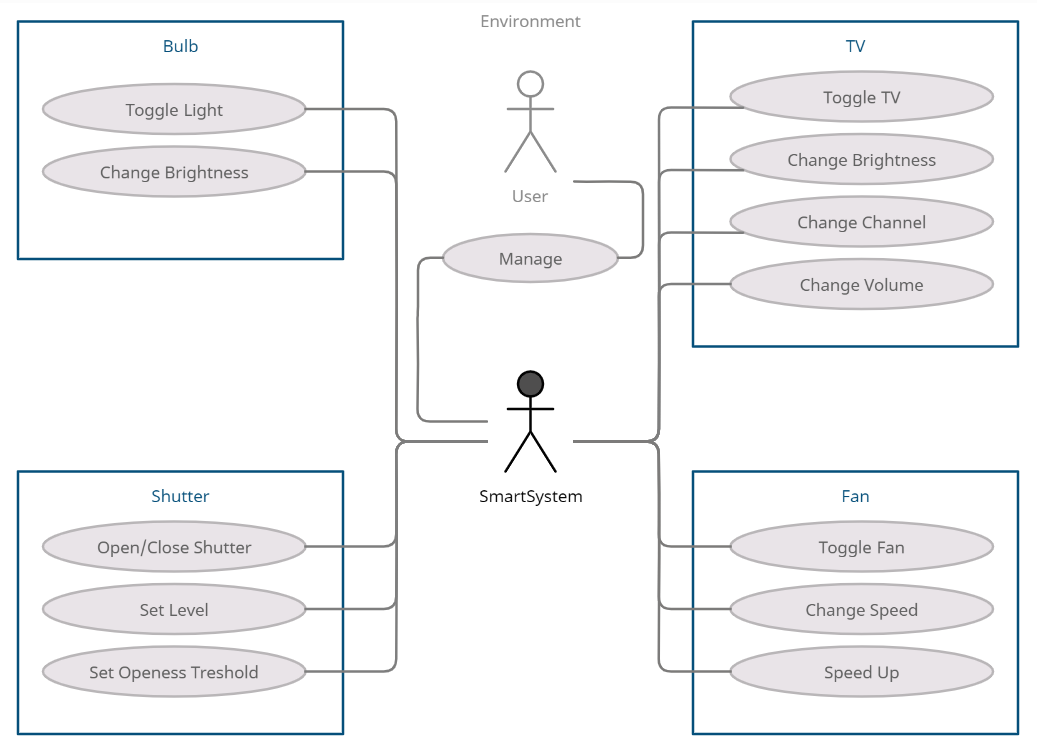
\includegraphics[scale=0.7]{eps/use-case-simple.png}}
	\caption{Casi d'uso del sistema in progettazione.}
	\label{fig:use-case}
\end{figure}

Ciò però risulta essere un livello \textit{base} e non prevede alcun tipo di astrazione. Si definiscono quindi anche alcuni esempi di azioni che possono essere eseguite all'interno di un sistema, indipendenti dalle Things attualmente posizionate nella stanza. Ovviamente, l'esito di un'operazione dipenderà se effettivamente vi sono Things capaci di raggiungere quell'obiettivo.

\begin{itemize}
	\item \textbf{illumina la stanza} - comando che, se portato a termine, deve aumentare la luminosità della stanza;
	\item \textbf{non mi sento sicuro} - comando che, se portato a termine, deve poter garantire una maggiore sicurezza all'interno della stanza;
	\item \textbf{modalità relax} - comando che, se portato a termine, aziona tutti i dispositivi che aiutano, in quell'istante, a rendere l'atmosfera più piacevole.
\end{itemize}

\section{Design di Dettaglio}

\subsection{Agenti}
Si prevede l'uso di un agente principale, il quale sarà responsabile dell'interazione tra l'utente e le Things aggiunte. Esso sarà in poche parole l'entità che gestisce l'attuale situazione nella stanza: attraverso dei piani raggiungerà gli obiettivi posti, sia quelli specifici che generici, in modo da accontentare l'utilizzatore. L'agente dovrà poter comunicare con un'interfaccia grafica per la gestione di questi comandi. Oltre ai piani, non vi sono particolari esigenze per ciò che riguarda il mondo degli Agenti, in quanto, come dalla sezione \ref{sec:artifacts} è previsto l'utilizzo di Artefatti per alcune funzionalità interne, anche per sottostare al \textit{Single Responsibility Principle}.

\subsection{Artefatti}
\label{sec:artifacts}
Si prevede l'utilizzo di alcuni Artefatti collegati all'agente principale, i quali svolgeranno i ruoli di:

\begin{itemize}
	\setlength\itemsep{-0.3em}
	\item ottenimento e l'interazione con le Things del sistema,
	\item visualizzazione dell'output (GUI).
\end{itemize}

Dovrebbe essere inoltre possibile l'auto-configurazione delle Thing inserite all'interno del sistema, ma per semplicità si presuppone l'atto di aggiunta come l'avvio del sistema stesso. Utilizzando poi le funzionalità del Framework scelto si possono definire modi per catturare anche questo aspetto più in dettaglio: utilizzando sempre \texttt{ThingWeb.io} è possibile progettare un Artefatto (o Agente) che faccia da endpoint per l'aggiunta (o creazione) di nuove Thing, utilizzando il protocollo REST. Si può, ad esempio, progettare un ulteriore file \texttt{.js} rispetto a quelli già presenti per le Thing implementate che, attraverso una chiamata \texttt{POST} su un ipotetico \textit{manager/things/create} esegui la funzionalità richiesta, simulando in modo più autentico il mondo reale. Rimarrebbe comunque il problema di come le Things possano raggiungere questo endpoint in modalità automatica, senza nessuna indicazione da parte dell'utente (o al contrario, di come l'endpoint possa accorgersi di nuove Things inserite all'interno del sistema): per fare un esempio, vi è comunque necessità di indicare la password della rete WiFi alla qual si vogliono connettere le Things e l'endpoint; a questo punto però vi è necessariamente un bisogno di configurarle manualmente, vanificando l'obiettivo della configurazione pienamente automatica.\\

Quindi, per concentrarsi più sulla dimostrazione delle potenzialità del framework, piuttosto che sugli aspetti di configurazione, si intendono le Things già presenti all'interno della stanza, ottenibili da un endpoint pre-configurato.



%%%%%%%%%%%%%%%%%%%%%%%%%%%%%%%%%%%%%%%%%non numera l'ultima pagina sinistra
\clearpage{\pagestyle{empty}\cleardoublepage}
\chapter{Proof of Concept - Realizzazione}           %crea il capitolo
%%%%%%%%%%%%%%%%%%%%%%%%%%%%%%%%%%%%%%%%%imposta l'intestazione di pagina
\lhead[\fancyplain{}{\bfseries\thepage}]{\fancyplain{}{\bfseries\rightmark}}  


\section{Configurazione}
Dati i requisiti e la volontà di utilizzare Kotlin come linguaggio di sviluppo, la configurazione del progetto richiede alcuni passaggi particolari che permettono un corretto funzionamento dell'applicazione in tutti gli IDE. Anche se alcuni potrebbero apparire privi di significato o inutili, servono in qualche modo a configurare meglio il progetto: vi è quindi necessità di esplorare perchè è necessario svolgere alcune operazioni affinché il tutto funzioni correttamente.

\subsection{Operazioni preliminari}
È necessario verificare che tutti i sottostanti requisiti siano soddisfatti:

\begin{itemize}
	\item si deve essere sicuri del fatto che Kotlin e JavaFX (in particolare, TornadoFX) siano la strada che si vuole percorrere nella realizzazione di questo progetto;
	
	\item aver installato e lanciato almeno una volta \textbf{IntelliJ} e \textbf{Eclipse}: le versioni sulle quali è stata configurata l'app sono rispettivamente 2020.2.3 e 4.16.0;
	\begin{itemize}
		\item su Eclipse bisogna installare il plugin per Kotlin e JaCaMo \cite{eclipse};
		
		\item su IntelliJ bisogna assicurarsi di abilitare il supporto per la programmazione in Kotlin;
	\end{itemize}

	\item avere le dipendenze impostate per lanciare applicazioni sotto Java versione 12.0.2 (testato con la versione 14 presentava problemi);
	\begin{itemize}
		\item sotto Windows, la variabile \texttt{JAVA\_HOME} dev'essere correttamente impostata per puntare alla versione 12.0.2;
	\end{itemize}

	\item effettuare un test di lancio dell'applicazione in modalità previste dalla guida ufficiale su JaCaMo \cite{jacamo};
	\begin{itemize}
		\item se l'applicazione non si avvia nemmeno in questa modalità, è abbastanza inutile procede;
	\end{itemize}
	
	\item è importante iniziare questa guida \textbf{prima} di creare del codice con JaCaMo.
\end{itemize}

\subsection{Configurazione progetto Eclipse + IntelliJ}
Anche se la guida ufficiale su come installare JaCaMo indica due modalità di creazione del progetto (sia da \texttt{gradle} che da \textit{Eclipse}), soltanto quella creata con \texttt{gradle} può essere letta correttamente da \textit{IntelliJ}, presentato però problemi di lettura da \textit{Eclipse}. Per affrontare questo problema bisogna impostare due progetti contemporaneamente (uno da \texttt{gradle} e l'altro da \textit{Eclipse}) e unirli subito dopo averli creati. Di seguito i passaggi elencanti in modo esaustivo:

\begin{enumerate}
	\item effettuare il download del file di configurazione del progetto\footnote{al momento il file risulta essere disponibile su \url{http://jacamo.sourceforge.net/nps/np09.zip}} direttamente dalla guida ufficiale \cite{jacamo};
	
	\item estrarre i file dall'archivio scaricato in una cartella della quale il percorso \textbf{non} contiene alcun spazio bianco (ad esemio un path valido potrebbe essere \texttt{C:/utenti/user/Desktop/np09});
	
	\item avviare \texttt{gradlew.bat} e aspettare il completamento del download di alcune dipendenze;
	
	\item quando richiesto, immettere il nome del progetto JaCaMo che si intende realizzare, utilizzando soltanto caratteri minuscoli e il simbolo \quotes{\_} (ad esempio \textit{smart\_room}); è necessario ricordarsi questo nome per i successivi passaggi;
	
	\item lasciar completare la configurazione finchè non si chiuderà o non chiederà di essere chiusa;
	
	\item \label{item:eclipse}lanciare \textit{Eclipse} \textbf{senza} aprire il progetto creato: avviare soltanto il programma;
	
	\item andare nella prospettiva di JaCaMo e creare un nuovo progetto JaCaMo da \textit{File > New > JaCaMo Project};
	
	\item nel campo \textit{Project Name} inserire \textbf{lo stesso identico nome} del progetto creato con \texttt{gradle} (in questo caso \textit{smart\_room}); assicurarsi inoltre che \textit{Agent} e \textit{Environment} siano impostati al valore \textit{centralized};
	
	\item dare conferma ed attendere la sua creazione;
	\begin{itemize}
		\item se Eclipse dovesse rispondere che esiste già un progetto così configurato, la soluzione più semplice è creare un workspace nuovo nel quale successivamente configurare questo progetto, ripercorrendo le istruzioni dal punto \ref{item:eclipse};
	\end{itemize}
	
	\item recarsi nella cartella dove il progetto \textit{Eclipse} è stato creato (in linea generale esso dovrebbe trovarsi nel workspace precedentemente utilizzato) e copiare tutti gli elementi presenti dentro la cartella del progetto;
	
	\item recarsi nella cartella dove il progetto \texttt{gradle} è stato creato (in questo esempio, su \texttt{C:/utenti/user/Desktop/np09}) e incollare dentro la cartella col nome del progetto (in questo esempio \textit{smart\_room}) i file copiati nel punto precedente;
	
	\item quando richiesto, \textbf{sovrascrivere i file};
	
	\item tornare su Eclipse (o riaprilo) ed \textbf{eliminare} il progetto creato con Eclipse, sia dall'anteprima del programma che dal disco: rimuovere ogni traccia dell'esistenza di questo progetto è essenziale;
	
	\item sempre su Eclipse, selezionare \textit{File/Open Projects from File System...} e recarsi all'interno della cartella del progetto \texttt{gradle}, dentro la cartella con il nome del progetto (in questo esempio si fa riferimento a \texttt{C:/utenti/user/Desktop/np09/smart\_room}): di conseguenza aprire il progetto e lasciare che l'importazione di esso abbia esito positivo;
	\begin{itemize}
		\item è essenziale eseguire questa operazione da \quotes{\textit{Open Projects from File System...}} in quanto \textit{Import} non funziona;
	\end{itemize}
	
	\item una volta caricato dovrebbe essere ben visibile nel visualizer di JaCaMo per Eclipse;
	\begin{itemize}
		\item questo non accade se importato direttamente dal progetto \texttt{gradle};
	\end{itemize}
	
	\item impostare il comando di lancio: sotto \textit{Run As} selezionare \textit{Run Configurations} e successivamente andare su \textit{Gradle Task}. All'interno di questa voce, immettere come \textit{Gradle Task} semplicemente \texttt{run} e come \\textit{Working Directory} indicare il valore\\
		\texttt{\${workspace\_loc:/<project\_name>}}, (in questo caso pari a \\
		\texttt{\$workspace\_loc:/smart\_room})
		
	\item avviare da \texttt{gradle}: se l'agente risponde \textit{Hello World!} è tutto configurato correttamente
\end{enumerate}

\subsection{Configurazione Kotlin IntelliJ + Eclipse}
La libreria sfrutta nativamente il linguaggio Java per cui sono necessari alcuni passaggi extra per poter utilizzare Kotlin come linguaggio di sviluppo. La seguente configurazione permette la compilazione Kotlin sia a livello di IntelliJ che Eclipse e non richiede la chiusura forzata dei programmi eventualmente aperti: essi verranno sincronizzati automaticamente.

\begin{enumerate}
	\item avviare IntelliJ e selezionare \textit{File/Open}: aprire di conseguenza la cartella col nome del progetto, situata all'interno della directory con il progetto \texttt{gradle} configurato in precedenza (in questo caso il path da aprire è  \texttt{C:/utenti/user/Desktop/np09/smart\_room});
	
	\begin{itemize}
		\item se richiesto, aprire la soluzione come progetto \textbf{gradle} e non Eclipse;
		
		\item sotto Windows IntelliJ potrebbe chiedere se migliorare le performance escludendo la cartella del progetto dall'antivirus: acconsentire o rifiutare in base alle proprie preferenze
	\end{itemize}

	\item dentro IntelliJ aprire il file \texttt{build.gradle}: se richiesto effettuare il \textit{fix}, dopodiché eseguirlo;
	\begin{itemize}
		\item se l'agente risponde \textit{Hello World!} si può procedere;
	\end{itemize}

	\item sempre dentro IntelliJ, seguendo la struttura del progetto, recarsi dentro \textit{src/env/tools} e creare una nuova classe Kotlin, chiamata ad esempio \textit{SampleClass};
	
	\item il programma chiederà in basso a destra se si vuole configurare il progetto per essere supportato da Kotlin: acconsentire selezionando la voce \quotes{\textit{as Kotlin (Java with Gradle module)}}, assicurandosi che nella successiva finestra sia abilitata l'opzione \textit{All modules containing Kotlin files} e che il compilatore Kotlin selezionato non sia sperimentale.
	\begin{itemize}
		\item in questo modo il file di \texttt{gradle} verrà automaticamente impostato per supportare Kotlin;
	\end{itemize}

	\item lanciare l'applicazione per controllare se tutto funziona correttamente;
	\begin{itemize}
		\item il primo lancio potrebbe essere più lungo, in quanto è possibile che delle dipendenze debbano essere scaricate;
		\item se non dovesse funzionare, si può provare ad aggiornare il valore di \textit{ext.kotlin\_version} a quello suggerito dall'IDE.
	\end{itemize}

Una nota importante riguardante l'intera procedura è che, mentre IntelliJ ha un supporto migliore per quanto riguarda Kotllin, Eclipse è più adatto per la gestione degli Agenti. Inoltre, per eseguire l'applicazione si dovrà utilizzare sempre \texttt{gradle}, in quanto provando a lanciare da Eclipse in modo tradizionale, le classi scritte in Kotlin mostreranno diversi errori di compilazione.
\end{enumerate}



\subsection{Configurazione JavaFx + TornatoFX}
Sfruttando Kotlin è possibile utilizzare le feature offerte da questo linguaggio, quali un supporto più agevole per la programmazione di interfacce grafiche. Per la configurazione di JavaFX occorrono i seguenti passi:

\begin{enumerate}
	\item aggiungere le seguenti dipendenze al file gradle:
	\begin{lstlisting}
	implementation "org.openjfx:javafx-base:14"
	implementation "org.openjfx:javafx-graphics:14"
	implementation "org.openjfx:javafx-controls:14"
	implementation "org.openjfx:javafx-fxml:14"
	\end{lstlisting}

	\item aggiungere alla voce \textit{buildscript.repositories}:
	\begin{lstlisting}
	mavenCentral()
	mavenLocal()
	maven {
		setUrl("https://plugins.gradle.org/m2/")
	}
	\end{lstlisting}

	\item aggiungere alla voce \textit{buildscript dependencies}:
	\begin{lstlisting}
	classpath "org.openjfx:javafx-plugin:0.0.9"
	\end{lstlisting}

	\item aggiungere sotto tutti i plugin esistenti la voce:
	\begin{lstlisting}
	apply plugin: "org.openjfx.javafxplugin"
	\end{lstlisting}

	\item nelle ultime righe del file \textit{gradle} aggiungere:
	\begin{lstlisting}
	javafx {
		version = "14"
		modules = [ 'javafx.controls' ]
	}
	\end{lstlisting}
\end{enumerate}

Successivamente, per configurare TornadoFX, una libreria che sfrutta a pieno le potenzialità di Kotlin applicate a JavaFx, si svolgono i seguenti passi:
\begin{enumerate}
	\item aggiungere alle dipendenze del progetto:
	\begin{lstlisting}
	implementation 'no.tornado:tornadofx:1.7.20'
	\end{lstlisting}

	\item cambiare la linea \textit{javafx \{ ... modules \}} in:
	\begin{lstlisting}
	modules = [ 'javafx.controls', 'javafx.graphics' ]
	\end{lstlisting}

	\item provare ad estendere la classe esempio creata in precedenza con l'entry point di TornadoFX (\texttt{:App()}); se il progetto parte è tutto configurato correttamente.
\end{enumerate}

Se qualcosa non dovesse funzionare, controllare se ogni punto della procedura è stato fatto. Si può inoltre tentare di spostare interamente il \textit{buildscript} all'inizio del file, prima della voce \textit{defaultTasks}. 


\section{Creazione del Main Agent}
L'agente principale si occuperà del lancio dell'assistente per l'utente. Esso conterrà intenzioni le quali permetteranno di eseguire sia le volontà generiche dell'utente che le specifiche operazioni sulle Things riconosciute dal sistema. La GUI è gestita attraverso un Artefatto, seguendo un buon esempio di \textit{blackboxing} delle funzionalità, in quanto l'Agente non può parlare direttamente con altre entità se non ulteriori Agenti o, appunto, gli Artefatti. Per la descrizione di quest'ultima, si rimanda al capitolo \ref{sec:gui}.\\

\subsection{Conoscenza di partenza}
Al suo interno, l'agente dichiara inizialmente la propria conoscenza di partenza. Essendo le Thing Description basate sull'ontologia SAREF, è possibile sfruttare questa intrinseca conoscenza per dichiarare all'agente alcune specifiche riguardanti Things che si può aspettare di avere. Si sottolinea comunque che, per essere completamente dinamici, l'agente potrebbe prendere come riferimenti ontologie meglio conosciute e richiedere direttamente ad esse classi di dispositivi di una cerca categoria.\\

\begin{lstlisting}
	guiStatus(false).						/* Gui is not ready yet */
	endpoint('http://localhost:8080/').		/* Endpoint where to connect */
	
	lightingType('saref:LightingDevice').	/* Devices that can make light */
	safetyAbility('saref:Safety').			/* Devices for safety */
	comfortAbility('saref:Comfort').		/* Devices that cam make comfort*/
\end{lstlisting}

\subsection{Piani e Goal}
Successivamente vengono dichiarati i piani. L'agente principale deve provvedere alla configurazione del sistema, che all'avvio deve poter visualizzare all'utente le Things connesse e interagire con esse. Si specifica quindi che si vogliono creare i due Artefatti di partenza e che si vuole attendere il completamento dell'avvio della GUI prima di procedere.

\begin{lstlisting}
/* Initial goal */
!start.

/* First goal: make Artifacts */
+!start : true
<-  makeArtifact("c0","display.MainViewArtifact", [], MainArtifact);
	focus(MainArtifact);
	makeArtifact("c1","things.ThingArtifact", [], ThingArtifact);
	focus(ThingArtifact).

/* Second goal: wait for GUI and init all the system */
+guiStatus(Condition) : Condition == true & endpoint(URL)
<-  .print("[AG] GUI is now ready: ", Condition);
	getAllThingDescriptions(URL, TDs);
	viewThingDescriptions(TDs).
\end{lstlisting}

L'interazione GUI-Utente avviene attraverso un Artefatto, che manda messaggi all'Agente per comunicargli gli eventi in arrivo. In questa parte verrà descritto soltanto il procedimento lato Agente, per quello relativo al \quotes{GUI Artifact} si rimanda al capitolo \ref{sec:gui}. Le richieste dell'utente vengono interpretate dall'Agente grazie ai messaggi contenenti la specifica funzionalità, in forma di una stringa testuale: ognuna di esse ha un piano base che esegue per completare la richiesta. Inoltre, per rendere il sistema completo di esempi, si eseguono le operazioni volute in tre modalità differenti:

\begin{itemize}
	\itemsep0em 
	\item \texttt{LightUp} eseguirà l'operazione di illuminare la stanza. Essa prenderà \u{soltanto un} elemento di una certa \u{tipologia}; nel caso specifico di un \textit{saref:LightingDevice}.
	\item \texttt{Safety} renderà la stanza più sicura. Essa prenderà \u{tutti i dispositivi} che servono per garantire una maggiore sicurezza; nel caso specifico, tutti i Device che hanno come proprietà \textit{saref:Safety}.
	\item \texttt{GoodVibes} porterà alla stanza un po' di relax e comfort. Essa prenderà \u{tutti i dispositivi} che servono per garantire un maggiore comfort all'interno della stanza; nel caso specifico, tutti i device che hanno come proprietà \textit{saref:Comfort}.
\end{itemize}

\begin{lstlisting}
/* Rsponding to GUI events */
+achieveIntention(Intention) : guiStatus(X) & X == true & Intention == "LightUp" & lightingType(La)
<-  .print("[AG] User wants to achieve something: ", Intention);
	!achieveWithTypology(La, true).

+achieveIntention(Intention) : guiStatus(X) & X == true & Intention == "Safety" & safetyAbility(Ha)
<-  .print("[AG] User wants to achieve something: ", Intention);
	!achieveWithAbility(Ha, false).
\end{lstlisting}

I due sotto-goal servono per realizzare effettivamente la funzionalità richiesta. Entrambi funzionano similmente, chiedendo prima di tutto tutti i device corrispondenti al criterio scelto, per poi selezionarne uno specifico (se richiesto) e di conseguenza di eseguire l'azione sul (o sui) device richiesto(i).

\begin{lstlisting}
+!achieveWithAbility(Ability, SelectOnlyOneThing) : endpoint(URL)
<-  findThingWithAbility(Ability, Things);
	selectBestThingForAbility(Ability, SelectOnlyOneThing, Things, SelectedThings);
	doOperation(SelectedThings, URL).

+!achieveWithTypology(Typology, SelectOnlyOneThing) : endpoint(URL)
<-  findThingWithTypology(Typology, Things);
	selectBestThingForTypology(Typology, SelectOnlyOneThing, Things, SelectedThings);
	doOperation(SelectedThings, URL).
\end{lstlisting}

Le operazioni definite in questi piani fanno riferimento all'Artefatto, descritto nel capitolo \ref{sec:things_artifact}

\section{Creazione Artefatti}

\subsection{GUI Artifact}
\label{sec:gui}
L'Artefatto con il quale si visualizza l'interfaccia utente. Si compone di proprietà osservabili e contiene riferimenti alla view creata sotto: questo perchè gli eventi potrebbero arrivare sia dall'esterno (ad esempio Agente), sia dall'interno (ad esempio, l'utente che preme il bottone). Per facilitare la creazione delle GUI, è stato predisposto un \texttt{GuiCreator}, il quale al momento può impostare il titolo, la dimensione e il \textit{controller} dell'interfaccia grafica. Essendo scritto in Kotlin, la creazione di essa risulta essere molto coincisa: quando è pronta, verrà impostata la proprietà interna dell'Artefatto che è già osservata dall'Agente; di conseguenza, appena la GUI si dichiara pronta, l'Agente è pronto per poter ricevere e mandare messaggi.

\begin{lstlisting}[language=Java]
// Create gui
with(GuiCreator.Builder()) {
	setTitle(GUI_TITLE)
	setDimensions(GUI_DIMENSION.first, GUI_DIMENSION.second)
}.build(MainView::class, guiController) { app, stage, view ->
	// After view creation, save references and show view
	this.app = app
	this.stage = stage
	this.view = view
	stage.show()
	execInternalOp(GUI_STATUS_OPERATION, true)
}
\end{lstlisting}

La GUI viene aggiornata attraverso l'esecuzione di un'operazione di aggiornamento su un campo \textit{booleano}, il quale viene definito prima di impostare l'interfaccia grafica. Questo parametro è osservato dall'Agente che sta tenendo il focus sull'Artefatto corrispondente all'interfaccia grafica osservata. Si vuole notare che non è possibile richiamare direttamente la funzione annotata con \textit{@INTERNAL\_OPERATION}, in quanto fa parte dell'Artefatto e non di una generica esecuzione Kotlin con le funzioni: vi è necessità di usare il metodo \texttt{execInternalOp} per eseguirla correttamente.

\begin{lstlisting}[language=Java]
// Init method for Artifact when property has its setup
@OPERATION
fun init {
	this.defineObsProperty(GUI_STATUS_PROPERTY, false)
	[... create gui]
}

// Execution of an internal operation
execInternalOp(GUI_STATUS_OPERATION, true)

// Implementation of the internal operation
@INTERNAL_OPERATION
fun onGuiStatusChange(status: Boolean) {
	getObsProperty(GUI_STATUS_PROPERTY).updateValue(status)
}
\end{lstlisting}

Attraverso un controller è possibile avere la comunicazione view - Artefatto. Esso dev'essere un'istanza della classe \texttt{Controller} - nell'esempio sottostante del \texttt{MainViewController}. Durante la creazione della view, il builder farà un controllo sull'appartnenza della view alla classe \texttt{ControllableView}, la quale definisce un unico metodo comune, \texttt{.setupController()}.

\begin{lstlisting}[language=Java, label=lst:view_artifact]
// Setting-up controller in the Artifact
private val guiController = object : MainViewController() {
	override fun onLightUpRoom() {
		execInternalOp(ACHIEVE_INTENTION_OPERATION, LIGHT_UP_INTENTION)
	}
	...
}

// Generic ControllerView abstract class
abstract class ControlledView<T> : View() where T : Controller {
	protected lateinit var controller: T
	fun setupController(controller: Controller) {
		try { this.controller = controller as T }
		 catch (exception: Exception) { throw IllegalArgumentException("Controller is not of requested type!") }
	}
}

// MainViewController abstract class
abstract class MainViewController : Controller() {
	abstract fun onLightUpRoom()
	...
}

// Builder cheking for ControllerView implementation
...
if (view is ControlledView<*>) {
	view.setupController(controller)
}
...

// View having its controller bounded to abstract class
class MainView : ControlledView<MainViewController>() { ... }
\end{lstlisting}

La comunicazione Artefatto-Agente viene invece definita tramite un unico metodo, in quanto le intenzioni sono differenziate dal loro tipo, grazie ad una stringa testuale. È la view a specificare, ad esempio, di voler raggiungere l'intenzione \texttt{LightUp}, mentre l'artefatto cattura questo evento. Nel codice \ref{lst:view_artifact} è presente infatti il metodo che esegue l'operazione interna dell'Artefatto: il parametro passato è semplicemente il nome della funzione associata a quell'operazione:

\begin{lstlisting}[language=Java]
@INTERNAL_OPERATION
fun onAchieveIntention(intention: String) {
	signal(INTENTION_SIGNAL, intention)
}
\end{lstlisting}

Per quanto riguarda invece le semplici interazioni oggetto-utente, senza intenzioni di alto livello, si predispone un'interfaccia essenziale con alcuni esempi di funzionalità. Non essendo lo scopo del progetto realizzare una GUI completamente funzionante, ma dimostrante le capacità, si implementano come esempio alcune delle possibile operazioni da svolgere. Si sottolinea come tutte le funzionalità che richiedono passaggi di parametri espliciti non sono state implementate.

\begin{figure}[h]
	\centering
	\makebox[\textwidth][c]{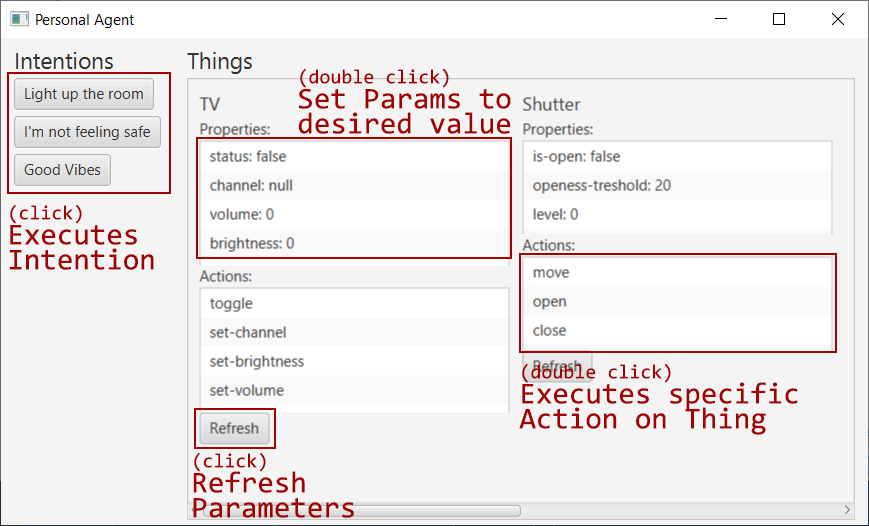
\includegraphics[width=1.3\textwidth]{eps/gui.png}}
	\caption{GUI essenziale per il funzionamento basilare del programma.}
	\label{fig:gui_implementation}
\end{figure}

Si sottolinea come tutte le funzionalità che richiedono passaggi di parametri espliciti non sono state implementate. Inoltre, per quanto riguarda le funzionalità base, quelle eseguite direttamente sulle Things, vi è un diretto passaggio da view a controller e l'esecuzione dell'operazione, senza il coinvolgimento (del tutto inutile) da parte dell'Artefatto e Agente. In un ottica più grande è ovvio che questo comportamento debba essere gestito dall'Agente stesso, in quanto è lui il responsabile del sistema; in un esempio di questo genere, si preferisce puntare sulla dimostrazione di funzionalità.

\subsection{Things Artifact}
L'artefatto responsabile all'ottenimento delle Things e comunicazione con esse. Anche se in principio vi era l'idea di utilizzare un Artefatto per ognuna delle Thing presenti in stanza, questa è stata abbandonata in favore di semplicità, anche grazie all'introduzione della semantica. Potenzialmente parlando, è possibile infatti  ricavare tutta la conoscenza necessaria direttamente dalla Thing Description: parametri da utilizzare, risorsa da chiamare e metodo con il quale farla. Avendo però fatto riferimento ad un'ontologia (SAREF) e avendo specificato tutte le Things all'interno di un modulo locale, si presuppone che esse vivano internamente all'ambiente di test e che quindi per la semplice dimostrazione delle funzionalità richieste è opportuno astrarre da questo aspetto, lasciando l'implementazione più dettagliata ad un eventuale approfondimento su questa tematica.\\

Di conseguenza, l'artefatto prevede 6 operazioni, tra le quali si possono trovare:
\begin{itemize}
	\item \texttt{getAllThingDescriptions} - interroga l'endpoint per farsi dare tutti gli URL delle Things attualmente connesse. Successivamente, per ogni URL ottenuto, salva la Thing Description di quel particolare Device.
	\item \texttt{doOperation} - esegue l'operazione (esempio GET o POST) sui Device indicati.
	\item \texttt{findThingWithAbility} - trova le Things che hanno una certa \quotes{abilità} (ad esempio, quella di illuminare o garantire comfort), indipendente dal tipo di oggetto. Utilizza query SPARQL per interrogare un endpoint nel quale è contenuta la conoscenza complessiva della stanza, in formato RDF.
	\item \texttt{findThingWithTypology} - simile a quella precedente, ma le Things richieste saranno di un specifico tipo, indipendente dalle abilità di quelli oggetti.
	\item \texttt{selectBestThingForAbility} - data una certa abilità, provvederà (se vi è necessità) la migliore Thing sulla quale eseguire l'azione, altrimenti, darà in risposta le Things trovate precedentemente. Utilizza query SPARQL per interrogare un endpoint nel quale è contenuta la conoscenza complessiva della stanza, in formato RDF.
	\item \texttt{selectBestThingForTypology} - simile a quella precedente, rispetto ad una certa tipologia di Device e non abilità.
\end{itemize}

È doveroso sottolineare che le funzionalità proposte servono per dimostrare le potenzialità di questo sistema e non ne rappresentano le piene capacità. È infatti possibile, grazie all'uso più esteso delle ontologie, a ricavare ancora più informazioni, anche grazie all'adozione di SWRL.


%%%%%%%%%%%%%%%%%%%%%%%%%%%%%%%%%%%%%%%%%non numera l'ultima pagina sinistra
\clearpage{\pagestyle{empty}\cleardoublepage}
\chapter{Conclusioni}           %crea il capitolo
%%%%%%%%%%%%%%%%%%%%%%%%%%%%%%%%%%%%%%%%%imposta l'intestazione di pagina
\lhead[\fancyplain{}{\bfseries\thepage}]{\fancyplain{}{\bfseries\rightmark}}  

Sin dai primi momenti di questa ricerca è stato chiara la volontà di poter coprire la maggior parte delle potenzialità offerte dal mondo analizzato: interoperabilità, sicurezza, funzionalità, dinamicità e conoscenza sono state le chiavi di tutta l'esplorazione eseguita. Il risultato ottenuto va ben oltre le specifiche che si possono ottenere in un semplice progetto-giocattolo, che tende soltanto a dimostrare alcune delle potenzialità del sistema per poi venir completamente dimenticato sia dal suo creatore che dalle persone che lo seguivano. Nel caso in discussione è stato possibile individuare molteplici proposte, difficoltà, soluzioni e alternative a problemi analizzati, contribuendo non solo a quello che risulta essere la realizzazione di prototipi in questo ambito, ma anche all'attiva partecipazione dello sviluppo delle librerie trattate durante lo studio.\\

Sono molteplici le difficoltà riscontrate, per le quali non si era previsto il tempo necessario: partendo da banali problematiche relative al mondo degli Agenti, finendo sulle numerose \textit{issue}\footnote{Come definito nel capitolo \ref{sec:issues}} aperte nei repository dei relativi Framework. Ma la ricerca è anche questo: trovarsi di fronte a difficoltà che non sono state comunemente affrontate, per le quali è necessario inventare nuove soluzioni e provvedere, in qualche modo, al raggiungimento dell'obiettivo posto.\\

Definire le Thing Description ha permesso di identificare le diversità che vi possono esistere tra oggetti e la necessità di avere un modo per capirne le funzionalità. L'aggiunta della semantica ha contribuito a valorizzare il significato e il peso della conoscenza del sistema, che ha permesso di identificare con estrema facilità i dispositivi di un certo tipo o quelli che svolgono una certa funzione, lasciando un campo tutto da esplorare per quel che riguarda ulteriori interrogazioni e inferenze di conoscenza.\\

Seguire un modello ad Agenti in un modo innovativo, configurato in maniera meno classica e seguendo un linguaggio meno comune, ma comunque compatibile, ha reso note le diverse difficoltà che è possibile incontrare durante lo sviluppo; scoperto però il procedimento corretto, è possibile far risparmiare tempo ad ulteriori programmatori che vorranno cimentarsi nella sperimentazione di questi framework, agevolando la configurazione e lo sviluppo di soluzioni sempre più innovative.\\

Il progetto, nel complesso, dimostra quanto sia possibile ottenere unendo i mondi di Web Semantico, Web of Thing e Pervasive Computing, senza però toccarne nemmeno la cima: è chiaramente impossibile cercare di implementare ogni questione relativa alle singole parti analizzate, in quanto per ognuna di esse è necessario predisporre un progetto che va ben oltre una semplice dimostrazione. Nel campo, vi sono diversi enti, aziende e gruppi di lavoro che stanno continuamente pensando a nuovi standard e/o linee guida sul mondo interconnesso che si sta creando: è del tutto improbabile che un singolo studente possa abbracciare l'interezza di questo sistema. Di conseguenza, è necessario sottolineare come il tutto porti ad avere più domande che risposte: rimangono ancora numerosi campi da coprire e lacune da riempire per poter dichiarare un sistema autonomo, indipendente, facilmente configurabile e auto-descrivente: sicuramente, la Thing Description è il punto di partenza per tutto ciò, e grazie all'unione della semantica e della visione pervasiva, i risultati attesi in futuro possono essere promettenti.\\

Comunque, la soddisfazione finale riguardante il progetto di ricerca e sviluppo va ben oltre le aspettative: nonostante i diversi cali subiti durante tutto l'iter, è possibile apprezzare come l'intero processo abbia portato ovunque a dei risultati anche non attesi:

\begin{itemize}
	\item è stato possibile capire le difficoltà, le sfide e le possibilità che si hanno a disposizione nella progettazione di sistemi eterogenei;
	\item è stato possibile constatare quanto la tecnologia attuale fatichi a perseguire l'obiettivo di interoperabilità abilitante anche alla semantica;
	\item diversi Framework hanno ricevuto feedback diretto da un utilizzatore che chiedeva più di un esempio-giocattolo;
	\item il mondo degli Agenti ha visto l'implementazione in Kotlin per una più efficiente prototipazione e realizzazione;
	\item il progetto finale offre diversi spunti per ampliamenti e potenziamenti dello stesso.
\end{itemize}

Nel complesso, quindi, si ritiene che l'iter che ha portato alle soprastanti conclusioni sia stato complesso, difficile e a volte demoralizzante, ma anche produttivo, stimolante e offrente diversi spunti per quello che risulterà essere un ulteriore ampliamento delle conoscenze in questo vastissimo campo.


%%%%%%%%%%%%%%%%%%%%%%%%%%%%%%%%%%%%%%%%%imposta l'intestazione di pagina
\renewcommand{\chaptermark}[1]{\markright{\thechapter \ #1}{}}
\lhead[\fancyplain{}{\bfseries\thepage}]{\fancyplain{}{\bfseries\rightmark}}

%\printbibliography[title={Whole bibliography}]
\printbibliography[keyword={article},title={Bibliografia}]
\printbibliography[keyword={online},title={Sitografia}]

%\bibliography{relazione}
%\bibliographystyle{siam}

\end{document}
